\documentclass[
  lang=cn,
  degree=bachelor,type=paper,
  openany,oneside
  % openright,blankleft,twoside
]{nuaathesis}

\graphicspath{{./fig/},{./logo/},{../logo/}}

\usepackage{algorithm}
\usepackage{algorithmic}

\iffalse
  % 本块代码被上方的 iffalse 注释掉,如需使用,请改为 iftrue
  % 使用 Noto 字体替换中文宋体、黑体
  \setCJKfamilyfont{\CJKrmdefault}[BoldFont=Noto Serif CJK SC Bold]{Noto Serif CJK SC}
  \renewcommand\songti{\CJKfamily{\CJKrmdefault}}
  \setCJKfamilyfont{\CJKsfdefault}[BoldFont=Noto Sans CJK SC Bold]{Noto Sans CJK SC Medium}
  \renewcommand\heiti{\CJKfamily{\CJKsfdefault}}
\fi

\iffalse
  % 本块代码被上方的 iffalse 注释掉,如需使用,请改为 iftrue
  % 在 XeLaTeX + ctexbook 环境下使用 Noto 日文字体
  \setCJKfamilyfont{mc}[BoldFont=Noto Serif CJK JP Bold]{Noto Serif CJK JP}
  \newcommand\mcfamily{\CJKfamily{mc}}
  \setCJKfamilyfont{gt}[BoldFont=Noto Sans CJK JP Bold]{Noto Sans CJK JP}
  \newcommand\gtfamily{\CJKfamily{gt}}
\fi


% 设置基本文档信息,\linebreak 前面不要有空格,否则在无需换行的场合,中文之间的空格无法消除
\nuaaset{
  title = {踝关节外骨骼的控制系统设计},
  author = {陈建宇},
  college = {自动化学院},
  advisers = {张娟娟 副教授,吕品 副教授},
  % applydate = {二〇一八年六月}  % 默认当前日期
  %
  % 本科
  major = {自动化},
  studentid = {051510626},
  classid = {0315106},
  % 硕/博士
  majorsubject = {\LaTeX},
  researchfield = {\LaTeX 排版},
  libraryclassid = {TP371},       % 中图分类号
  subjectclassid = {080605},      % 学科分类号
  thesisid = {1028704 18-S000},   % 论文编号
}
\nuaasetEn{
  title = {Design of Control System for Ankle Exoskeletons},
  author = {JianYuChen},
  college = {NUAA},
  majorsubject = {Automation},
  advisers = {Prof.~JuanJuanZhang},
  degreefull = {Master of Engineering},
  % applydate = {June, 8012}
}

% 摘要
\begin{abstract}
  外骨骼是一种用来提高人体机能的可穿戴设备,在军事作战、医疗康复等领域具有重要意义。提高人机交互的舒适性与安全性,为当前外骨骼领域的研究热点。本文研究对象为一种踝关节式外骨骼,在现有机械结构的基础上,对外骨骼传感系统、力矩控制方法、人在环中优化进行了研究。

  可靠、准确、稳定的人机交互数据对外骨骼而言至关重要。本文首先搭建了外骨骼的传感系统。针对所研究的踝关节式外骨骼,使用应变片测量外骨骼对人体施加的力矩,通过足底开关和惯性测量单元分析人体步态运动信息,通过EMG信号测量肌肉的激活水平。

  在传感系统的基础上,本文对外骨骼的力矩控制方法进行了研究。力矩控制由上层控制器与底层控制器组成,上层控制器用来产生期望力矩曲线,底层控制器实现对期望力矩曲线的跟踪。对于上层控制器,本文采用基于时间的直接力矩控制,并通过三次函数插值得到期望力矩曲线。针对底层控制器,本文提出了三种控制算法,设计了四种不同组合的控制器,通过实验发现融合三种控制算法的控制器具有较好的力矩跟踪效果。

  最后,本文研究了人在环中的参数优化方法。针对最佳助力模式因人而异的问题,本文以穿戴者的肌肉激活水平为目标函数,使用贝叶斯优化外搜寻最佳助力参数。实验表明,外骨骼系统能够在五分钟内寻找到最佳助力参数。在最佳助力参数下,受试者肌肉激活度平均下降12.2\%。

\end{abstract}
\keywords{外骨骼, 力矩控制, 人在环中优化}

\begin{abstractEn}
  Exoskeletons are wearable device used to enhance human mobility,which are significant in military, medical rehabilitation and many other fields.Improving the comfort and safety during human-machine interaction has become a hotspot in exoskeleton research.The research object of this paper is an ankle type exoskeleton.Based on the existing mechanical structure of an ankle exoskeleton,we study the sensing system,torque control method and human-in-loop optimization.

  Accurate and reliable sensor information is critical for exoskeleton.In this paper,we first develop a sensing system.The torque exerted on exoskeleton was measured by strain gauge,human gait information was analyzed by plantar switch,and muscle activation level was measured by EMG signal.

  Based on the sensing system,we study torque control method,which consists of upper controller and lower controller.The upper controller is used to generate desired torque curve,and the lower controller is used for tracking the desired torque curve.This paper adopts the direct torque control based on time,and obtains the desired torque curve by cubic spline interpolation.We proposes three control algorithms and design four different combinations of lower controller.Through experiments,we found that the controller contains all three algorithms has better torque tracking performance.

  Finally,we study human-in-loop optimization.We find that optimal assistance mode varies from person to person,which can be searched by optimization method.In the paper,the target function is human muscle activation level,and Bayesian Optimization was chosen to search optimal assistance.During five experiments,the exoskeleton system successfully searched the optimal assistance mode in five minutes.Under optimal assistance parameters,the muscle activation level of human subject decreased by 12.2\% on average.
\end{abstractEn}
\keywordsEn{exoskeleton, torque control, human in loop optimization}

% 请按自己的论文排版需求,随意修改以下全局设置

\usepackage{subfig}
\usepackage{rotating}
\usepackage[usenames,dvipsnames]{xcolor}
\usepackage{tikz}
\usepackage{pgfplots}
\pgfplotsset{compat=1.16}
\pgfplotsset{
  table/search path={./fig/},
}
\usepackage{ifthen}
\usepackage{longtable}
\usepackage{siunitx}
\usepackage{listings}
\usepackage{multirow}
\usepackage[bottom]{footmisc}
\usepackage{pifont}

\lstdefinestyle{lstStyleBase}{%
  basicstyle=\small\ttfamily,
  aboveskip=\medskipamount,
  belowskip=\medskipamount,
  lineskip=0pt,
  boxpos=c,
  showlines=false,
  extendedchars=true,
  upquote=true,
  tabsize=2,
  showtabs=false,
  showspaces=false,
  showstringspaces=false,
  numbers=left,
  numberstyle=\footnotesize,
  linewidth=\linewidth,
  xleftmargin=\parindent,
  xrightmargin=0pt,
  resetmargins=false,
  breaklines=true,
  breakatwhitespace=false,
  breakindent=0pt,
  breakautoindent=true,
  columns=flexible,
  keepspaces=true,
  framesep=3pt,
  rulesep=2pt,
  framerule=1pt,
  backgroundcolor=\color{gray!5},
  stringstyle=\color{green!40!black!100},
  keywordstyle=\bfseries\color{blue!50!black},
  commentstyle=\slshape\color{black!60}}

%\usetikzlibrary{external}
%\tikzexternalize % activate!

\newcommand\cs[1]{\texttt{\textbackslash#1}}
\newcommand\pkg[1]{\texttt{#1}\textsuperscript{PKG}}
\newcommand\env[1]{\texttt{#1}}

\theoremstyle{nuaaplain}
\nuaatheoremchapu{definition}{定义}
\nuaatheoremchapu{assumption}{假设}
\nuaatheoremchap{exercise}{练习}
\nuaatheoremchap{nonsense}{胡诌}
\nuaatheoremg[句]{lines}{句子}

% \includeonly{content/start,}

\begin{document}

\makecover
\makedeclare
\frontmatter
\makeabstract
% 如果需要调整目录层级数量的话,取消下一行注释,数字含义: 0=chapter, 1=section, 2=subsection
% \setcounter{tocdepth}{1}
\nuaatableofcontents

\mainmatter

%# -*- coding: utf-8-unix -*-
\chapter{简介}\label{chap:intro}

这是南京航空航天大学(非官方)本科生学位论文\LaTeX 模板,当前版本是\version。本模板由\nuaathesis~Group共同开发,模板文档由Old Jack撰写。

本模板最早可以追溯到人人网上的一篇博客\footnote{\url{http://bit.ly/2rGOhf6}},由黄大宁、邓欣珂、徐添豪、石坤四人共同开发完善,参考了当时东南大学的\seuthesix 模板;除此之外在Github上也可以找到一个repo\footnote{\url{https://github.com/nuaa803/nuaa-thesis}},由Felix Ding、Jun Wang、Jackie Hou三位老师和Vevi Zhong同学共同维护,但是repo中的.cls和.sty文件是空文件。

回顾人人网的模板,没有直接提供nuaa.png和nuaa.bst文件,可以使用强制编译的方法生成文件,但是缺少左上角南航字样,参考文献格式也不符合标准。除此之外,旧模板使用了已经被放弃使用的CJK宏包,因此在编译\verb+\Unicode{}+命令时会出错,代码的阅读性和维护性也不如现在的ctex和xeCJK。由于上述原因,许多初次使用\LaTeX 和使用经验不多的同学,在一开始就放弃了使用旧版模板进行毕业设计的书写及排版。

基于南航无可用\LaTeX 学位模板可用的现状,\nuaathesis~Group基于旧\oldnuaathesis 模板、现东南大学的\seuthesix 模板和上海交通大学的SJTU Thesis模板,对模板进行了二次开发,基本实现了学士学位论文的模板。\nuaathesis~Group现有成员短期内不计划开发团队报告、硕士博士学位论文等其他文档的\LaTeX 模板,留给后续成员以及其他有需要、有能力的南航学子以后开发。

现在\nuaathesis 模板的代码托管在Github\footnote{\url{https://github.com/jackwzh/nuaathesis}}上,如有修改建议或者其他要求欢迎在Github上开issue或提pull request,\nuaathesis~Group会尽快回复,并酌情处理您的要求。

本模板基于Windows~10平台开发,使用MiKTeX v2.9发行版,所使用的宏包均跟进到最新版本。Linux平台由张一白使用\TeX Live测试,macOS平台由王成欣进行了测试,目前尚未出现任何问题。本模板尚未在Windows平台使用\CTeX / \TeX Live进行测试,如出现问题,请自行Google、Bing、Baidu搜索解决方法。学会使用搜索引擎、熟练阅读外文是一个学生最基本的能力,更是一个\LaTeX 使用者得以立足和前进的根本。

\nuaathesis~Group非常欢迎有其他南航的\LaTeX 使用者加入到本模板的开发与维护当中来,不断完善模板,为南航广大学子造福!

\section{模板使用}
\subsection{准备工作}
\begin{itemize}
  \item \TeX 发行版:Windows 系统推荐使用MiKTeX和\TeX Live这两种发行版,前者占用空间小,只在有宏包缺失情况下才进行下载,后者占用空间大,但基本无需担心宏包缺失。Linux系统(Arch系除外)推荐手动安装\TeX Live发行版,官方源中的TeXLive版本跟进较慢。macOS可以参考SJTU Thesis中的介绍。
  \item \TeX 知识:本说明文档提供\TeX 使用的例子,但不能解决所有的问题,因此使用前请自行学习\TeX~\&~\LaTeX 相关知识。
\end{itemize}

\subsection{模板编译}

\textbf{切记使用\XeLaTeX 进行编译。}使用\XeLaTeX 和\hologo{BibTeX}在文档中加入参考文献的流程可参考如下命令:

\begin{lstlisting}[basicstyle=\small\ttfamily, caption=手动逐次编译, numbers=none]
xelatex -no-pdf .tex文件名
biber --debug .tex文件名
xelatex .tex文件名
xelatex .tex文件名
\end{lstlisting}

使用\XeLaTeX 引擎编译可以直接通过各\LaTeX 编辑器实现,如:TeXworks,TeXmaker,TeXStudio,Emacs+插件,Atom+插件等等。biber命令需使用Windows的cmd/Power Shell、Linux和macOS下的bash实现。Windows平台可以自行编写简单的.bat批处理文件来实现。

使用biber需注意:\textbf{.bib文件内的文件记录必须在.tex文件中被引用,不引用的记录不要因为懒而不去除,否则将编译失败}

目录内容需要编译两次才能正常显示,原因推断为早期的电脑内存不够,所以将目录的生成分成了两步来进行。

\subsection{模板文件结构}
\begin{itemize}[noitemsep,topsep=0pt,parsep=0pt,partopsep=0pt]
  \item .tex文件:主文件,chapter下有各个章节的文件,强烈建议将文章模块化,方便调试与版本管理。
  \item .cls、.cfg文件:模板定义文件
  \item .bib文件:参考文献数据库文件
  \item figure文件夹:存放要插入的图片,其中nuaa.png不可删除
\end{itemize}

\chapter{外骨骼数据采集与步态分析系统}

外骨骼是一个融合各种传感器的智能系统,可靠的传感器数据才能保证控制算法的性能。本章针对研究的踝关节式外骨骼搭建了一套传感器系统,包括以dSPACE为核心的处理器、测量外骨骼力矩的应变电桥、测量步态周期的足底开关、惯性测量单元IMU、表面肌电信号sEMG等,如图2.1所示。

\begin{figure}[htb]
    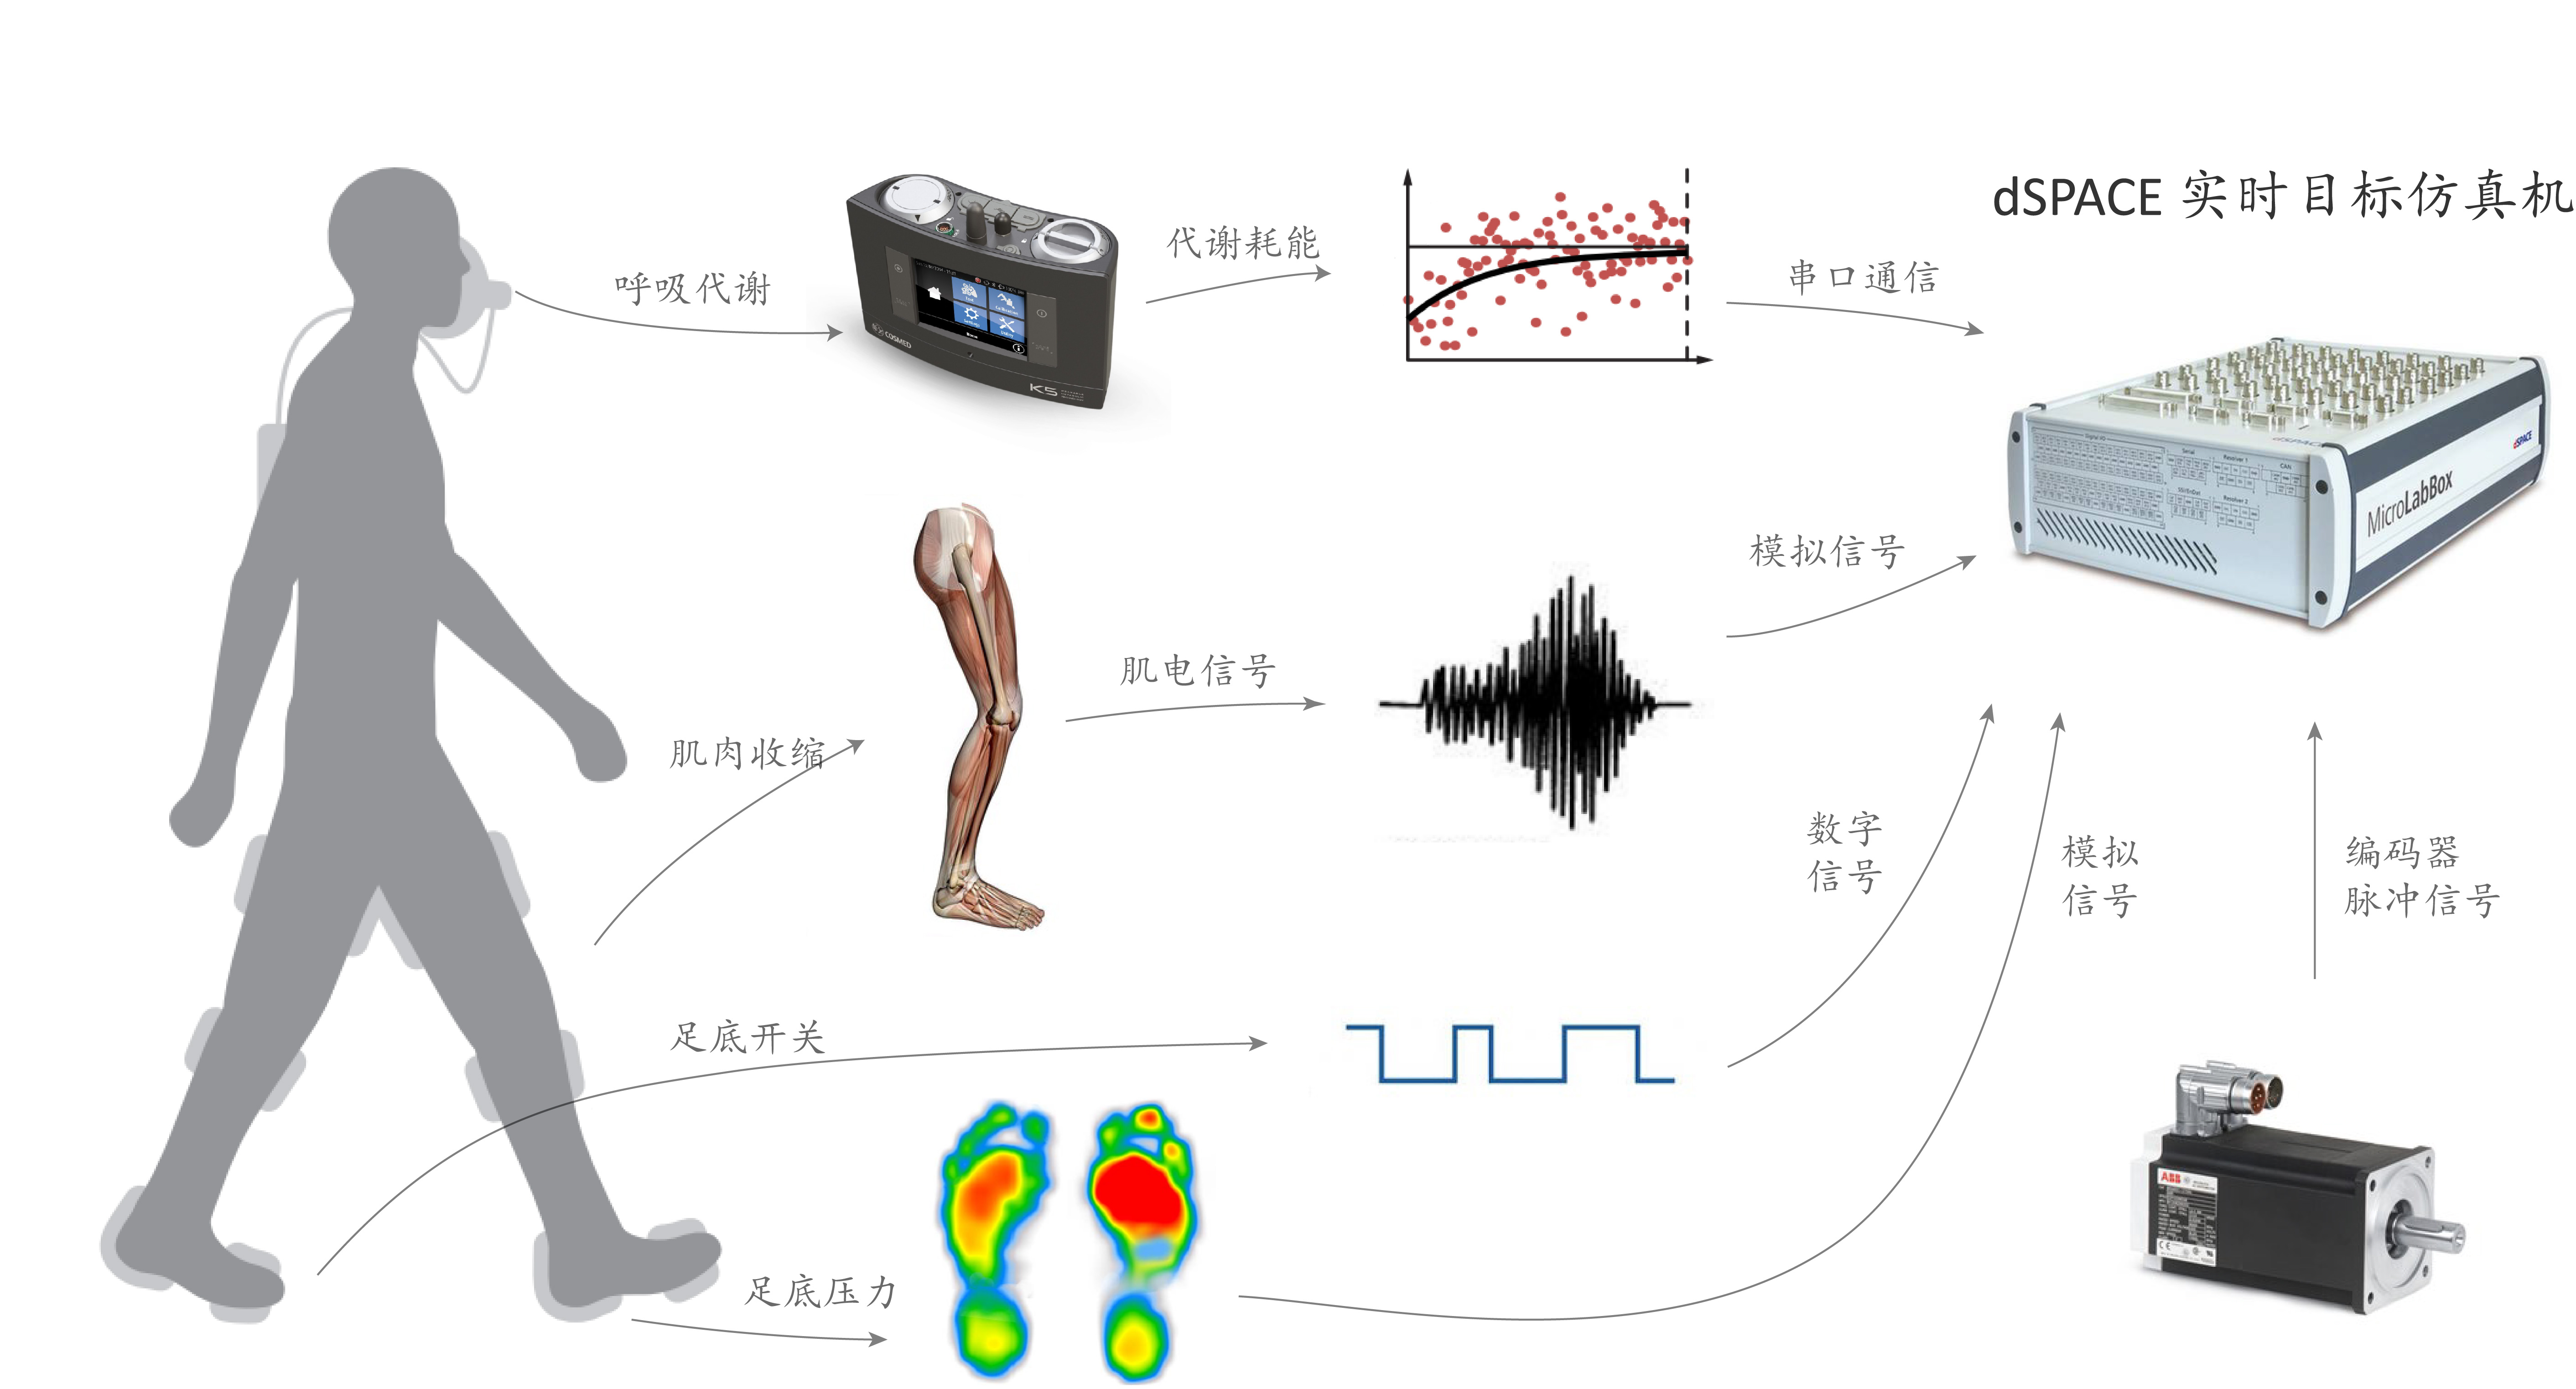
\includegraphics[width=15cm]{fig/f27.jpg}
    \caption{踝关节外骨骼的数据采集系统}
    \label{fig:mark}
\end{figure}

\section{dSPACE实时目标机MicroLabBox}

实时目标机是由德斯拜斯(dSPACE)公司开发的一套基于MATLAB/Simulink的控制系统开发及半实物仿真软硬件工作平台,它可以方便的与Matlab/Simulink进行连接,实现快速控制原型(RCP)或硬件在环仿真(HIL)。dSPACE通过Simulink进行控制算法的快速开发、代码生成与测试调试,具有强实时性、可靠性高、扩充性好的特点,目前已广泛应用于汽车、机器人、航空航天等领域。

\subsection{dSPACE的硬件平台}

\begin{figure}[htb]
    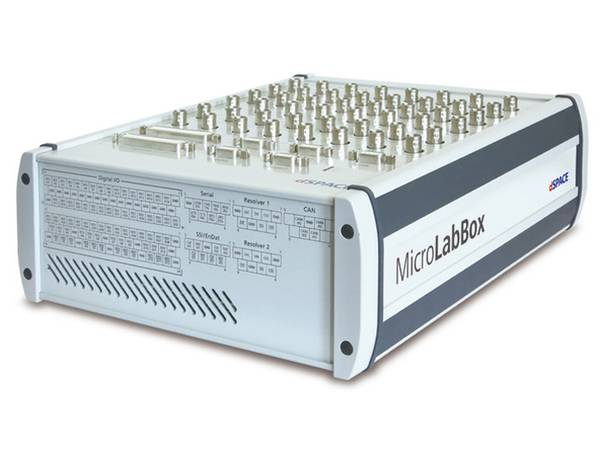
\includegraphics[width=8cm]{fig/f21.jpeg}
    \caption{dSPACE的实时目标机MicroLabBox}
    \label{fig:mark}
\end{figure}

MicroLabBox是dSPACE面向实验室推出的一款紧凑型实时仿真平台,如图2.1所示,具有高速的计算能力和快速的输入输出特性。CPU采用2GHz双核实时处理器(Freescale Power QorIQ 5020),最快可以实现15us的闭环控制周期,同时还可以使用内部集成的FPGA加速并行计算。MicroLabBox同时具有丰富的外设,48通道数字I/O接口、32通道模拟量输入接口、16通道模拟量输出接口,同时配有2个CAN总线收发器、1个RS-232串口、一个网络接口、6通道正交编码器接口等。除此之外,MicroLabBox中集成的稳压电源可以为传感器进行供电,使系统使用起来更加方便。

\subsection{dSPACE的软件平台}
(1)实时接口RTI

MicroLabBox与Simulink的连接是通过实时接口RTI来实现的。它可以看做是Simulink下关于MicroLabBox的一些模块,通过这些模块可以实现对MicroLabBox各种I/O接口的配置与初始化,并可以与Simulink中的其他模块,如控制模块、滤波模块相连接,从而实现数据采集与处理和控制系统的搭建。模型搭建完毕后,可以通过调用MATLAB的RTW工具对模型进行编译,自动生成适用于MicroLabBox的目标代码,并下载到MicroLabBox中完成Simulink模型预期实现的功能。
    
(2)ControlDesk

ControlDesk是dSAPCE公司开发的一种图形化的人机交互软件,能够提供虚拟示波器、虚拟按钮、虚拟表盘等功能,如图2.2所示。根据ControlDesk提供的各种工具,用户可以快速设计出适合项目的可视化界面,方便的对程序中的变量进行监控、修改参数、记录数据。

\begin{figure}[htb]
    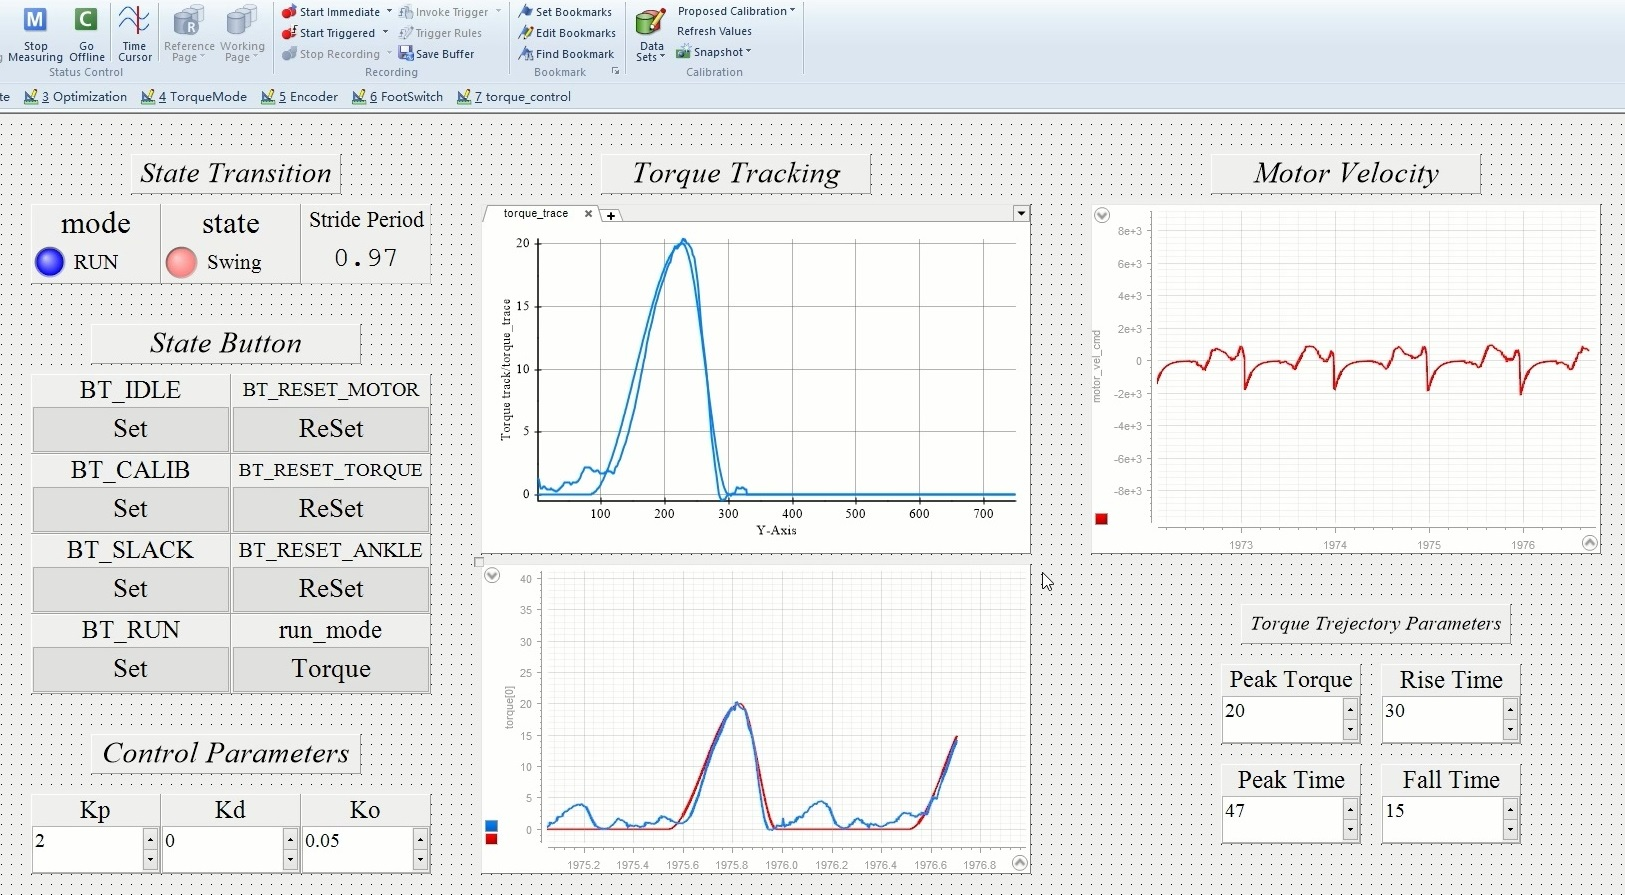
\includegraphics[width=14cm]{fig/f22.jpg}
    \caption{dSPACE的实时目标机MicroLabBox}
    \label{fig:mark}
\end{figure}

由于MicroLabBox可以借助Simulink以模块化的方式进行开发,并可以利用ControlDesk快速设计出对应的上位机界面,因此本文工作将以MicroLabBox为核心,进行数据采集、处理与外骨骼控制。

\section{外骨骼力矩测量}

\begin{figure}[htb]
    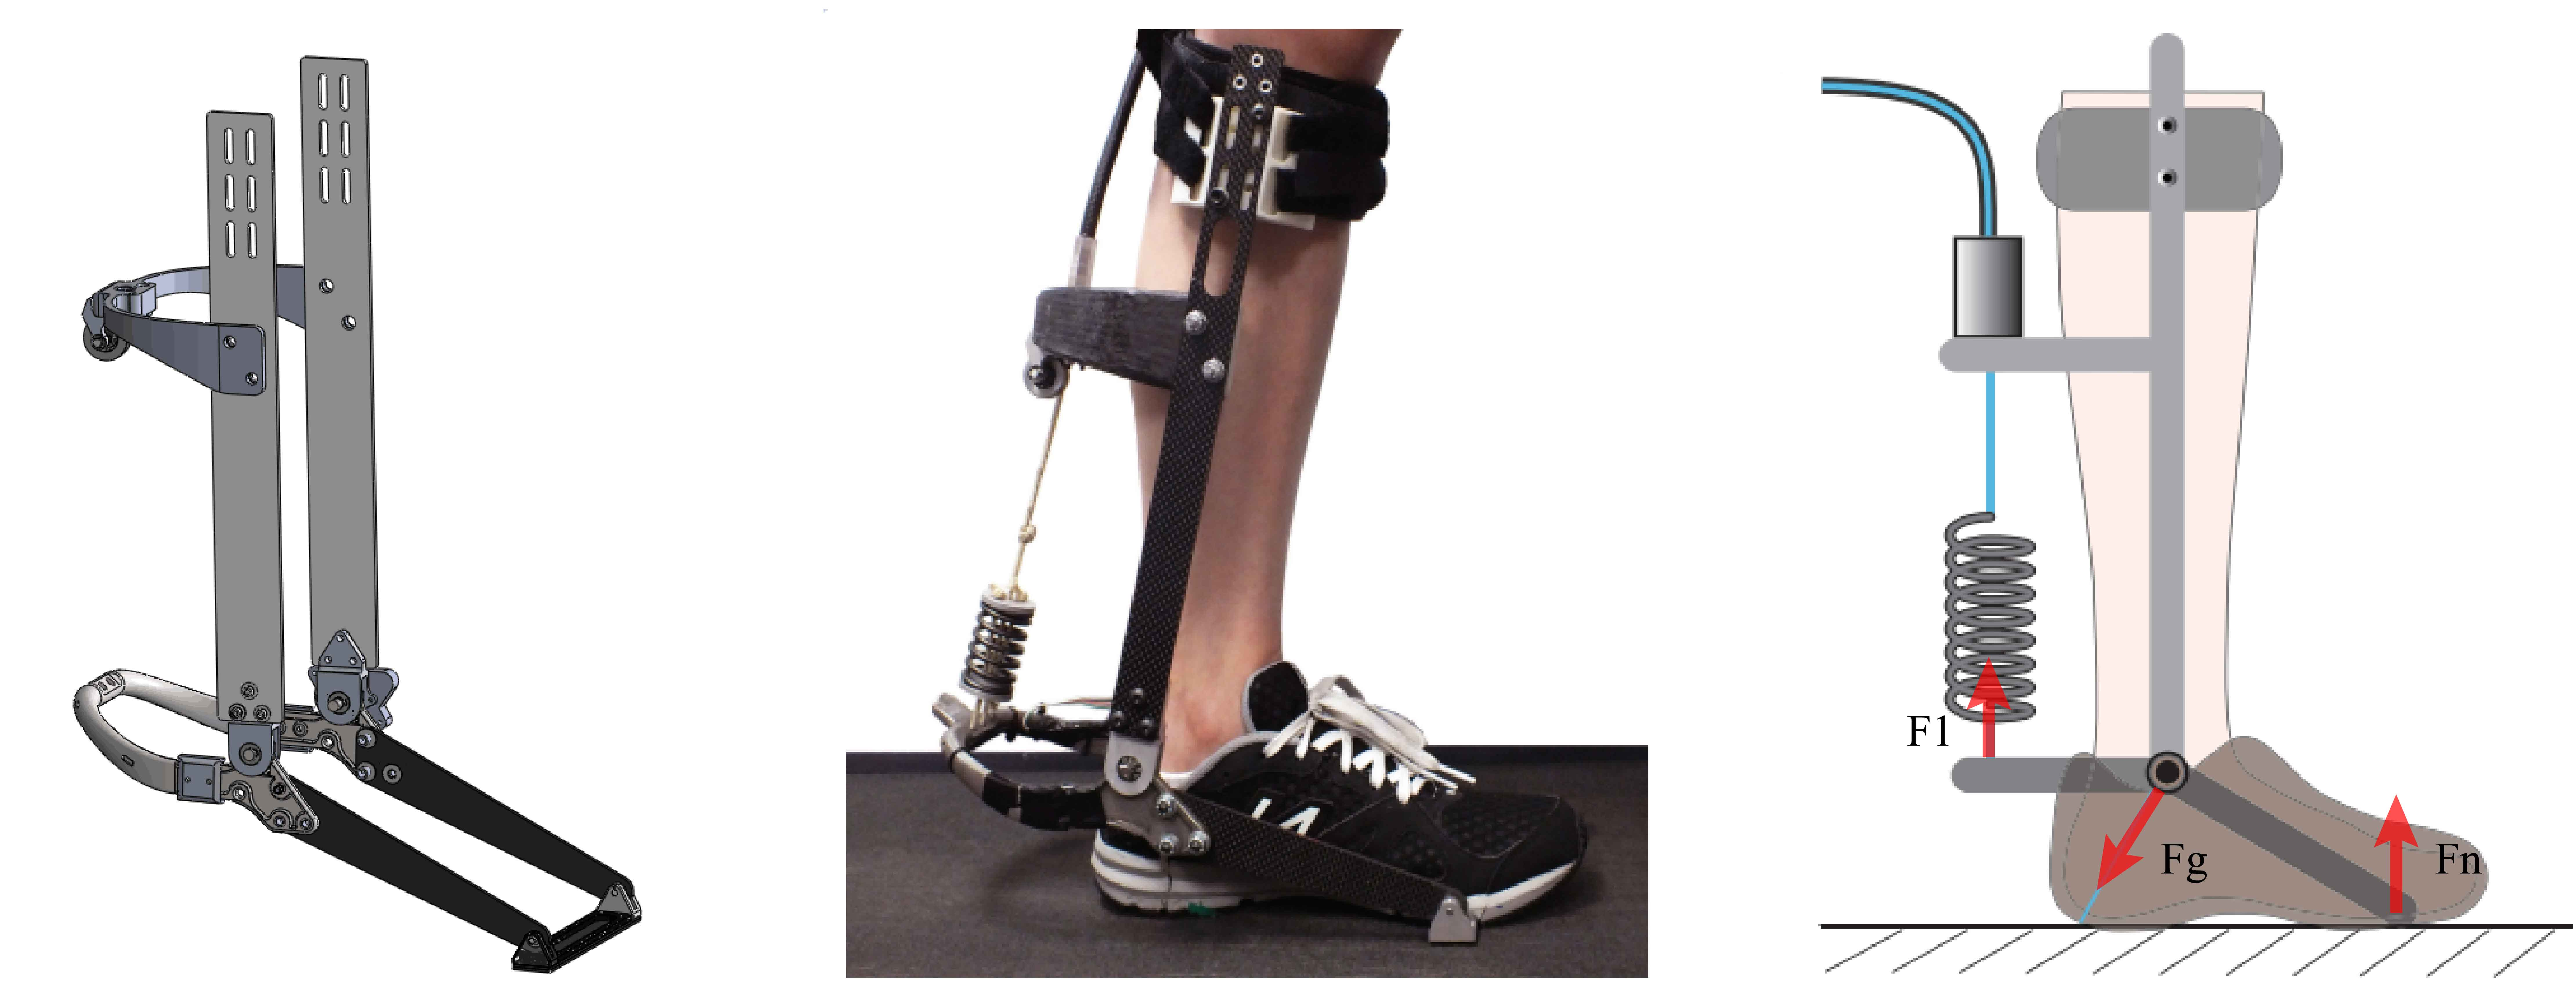
\includegraphics[width=14cm]{fig/f23.jpg}
    \caption{dSPACE的实时目标机MicroLabBox}
    \label{fig:mark}
\end{figure}

为了现实外骨骼的力矩控制,必须要对人机之间的交互力矩加以测量。外骨骼的结构与受力分布如图2.3所示。当电机通过鲍登线和SEA对外骨骼和穿戴者施加作用力$F1$时,由材料力学可知外骨骼的钛合金悬臂会在拉力的作用下发生变形,如图2.4 a)所示。通过应变片测量出钛合金悬臂的变形程度,即可得到电机施加的驱动力矩。

\begin{figure}[htb]
    \subfloat[外骨骼悬臂在拉力作用下发生变形]{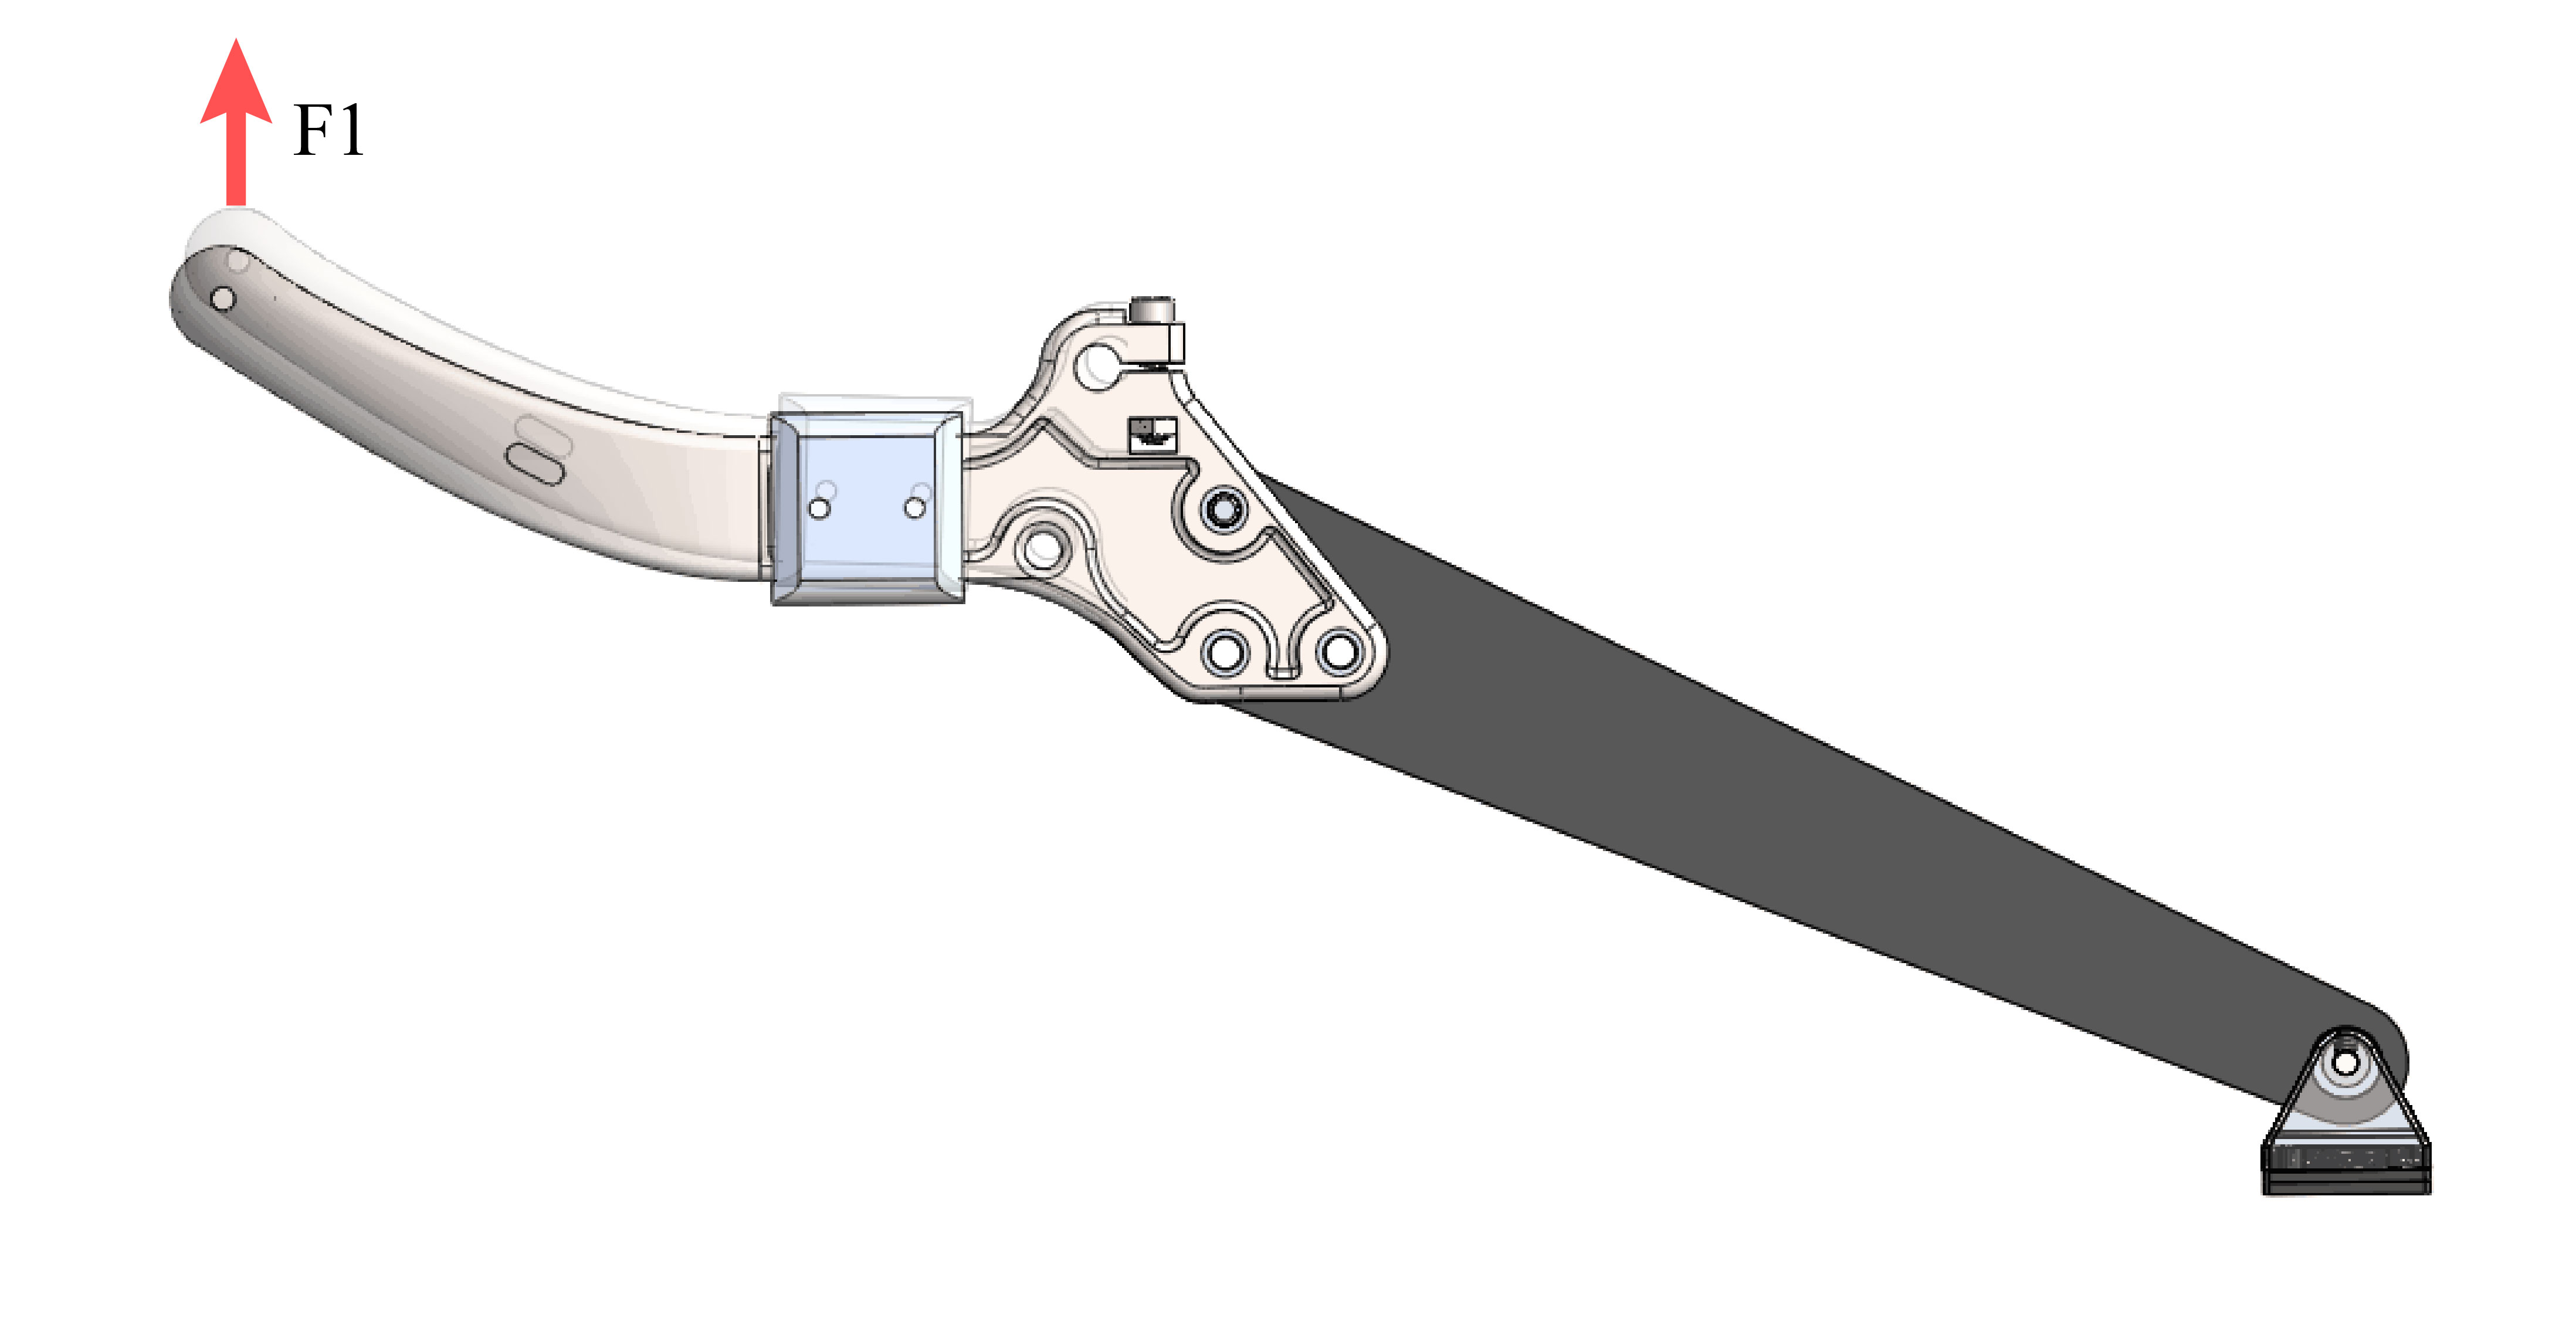
\includegraphics[width=7.5cm]{fig/f24.jpg}}\quad
    \subfloat[应变电桥的安装位置]{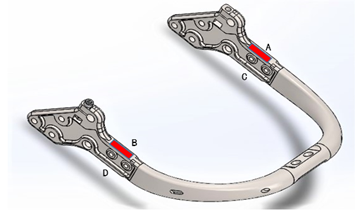
\includegraphics[width=6cm]{fig/f25.png}}
    \caption{外骨骼力矩测量原理}
    \label{fig:subfigss}
\end{figure}

\begin{figure}[htb]
    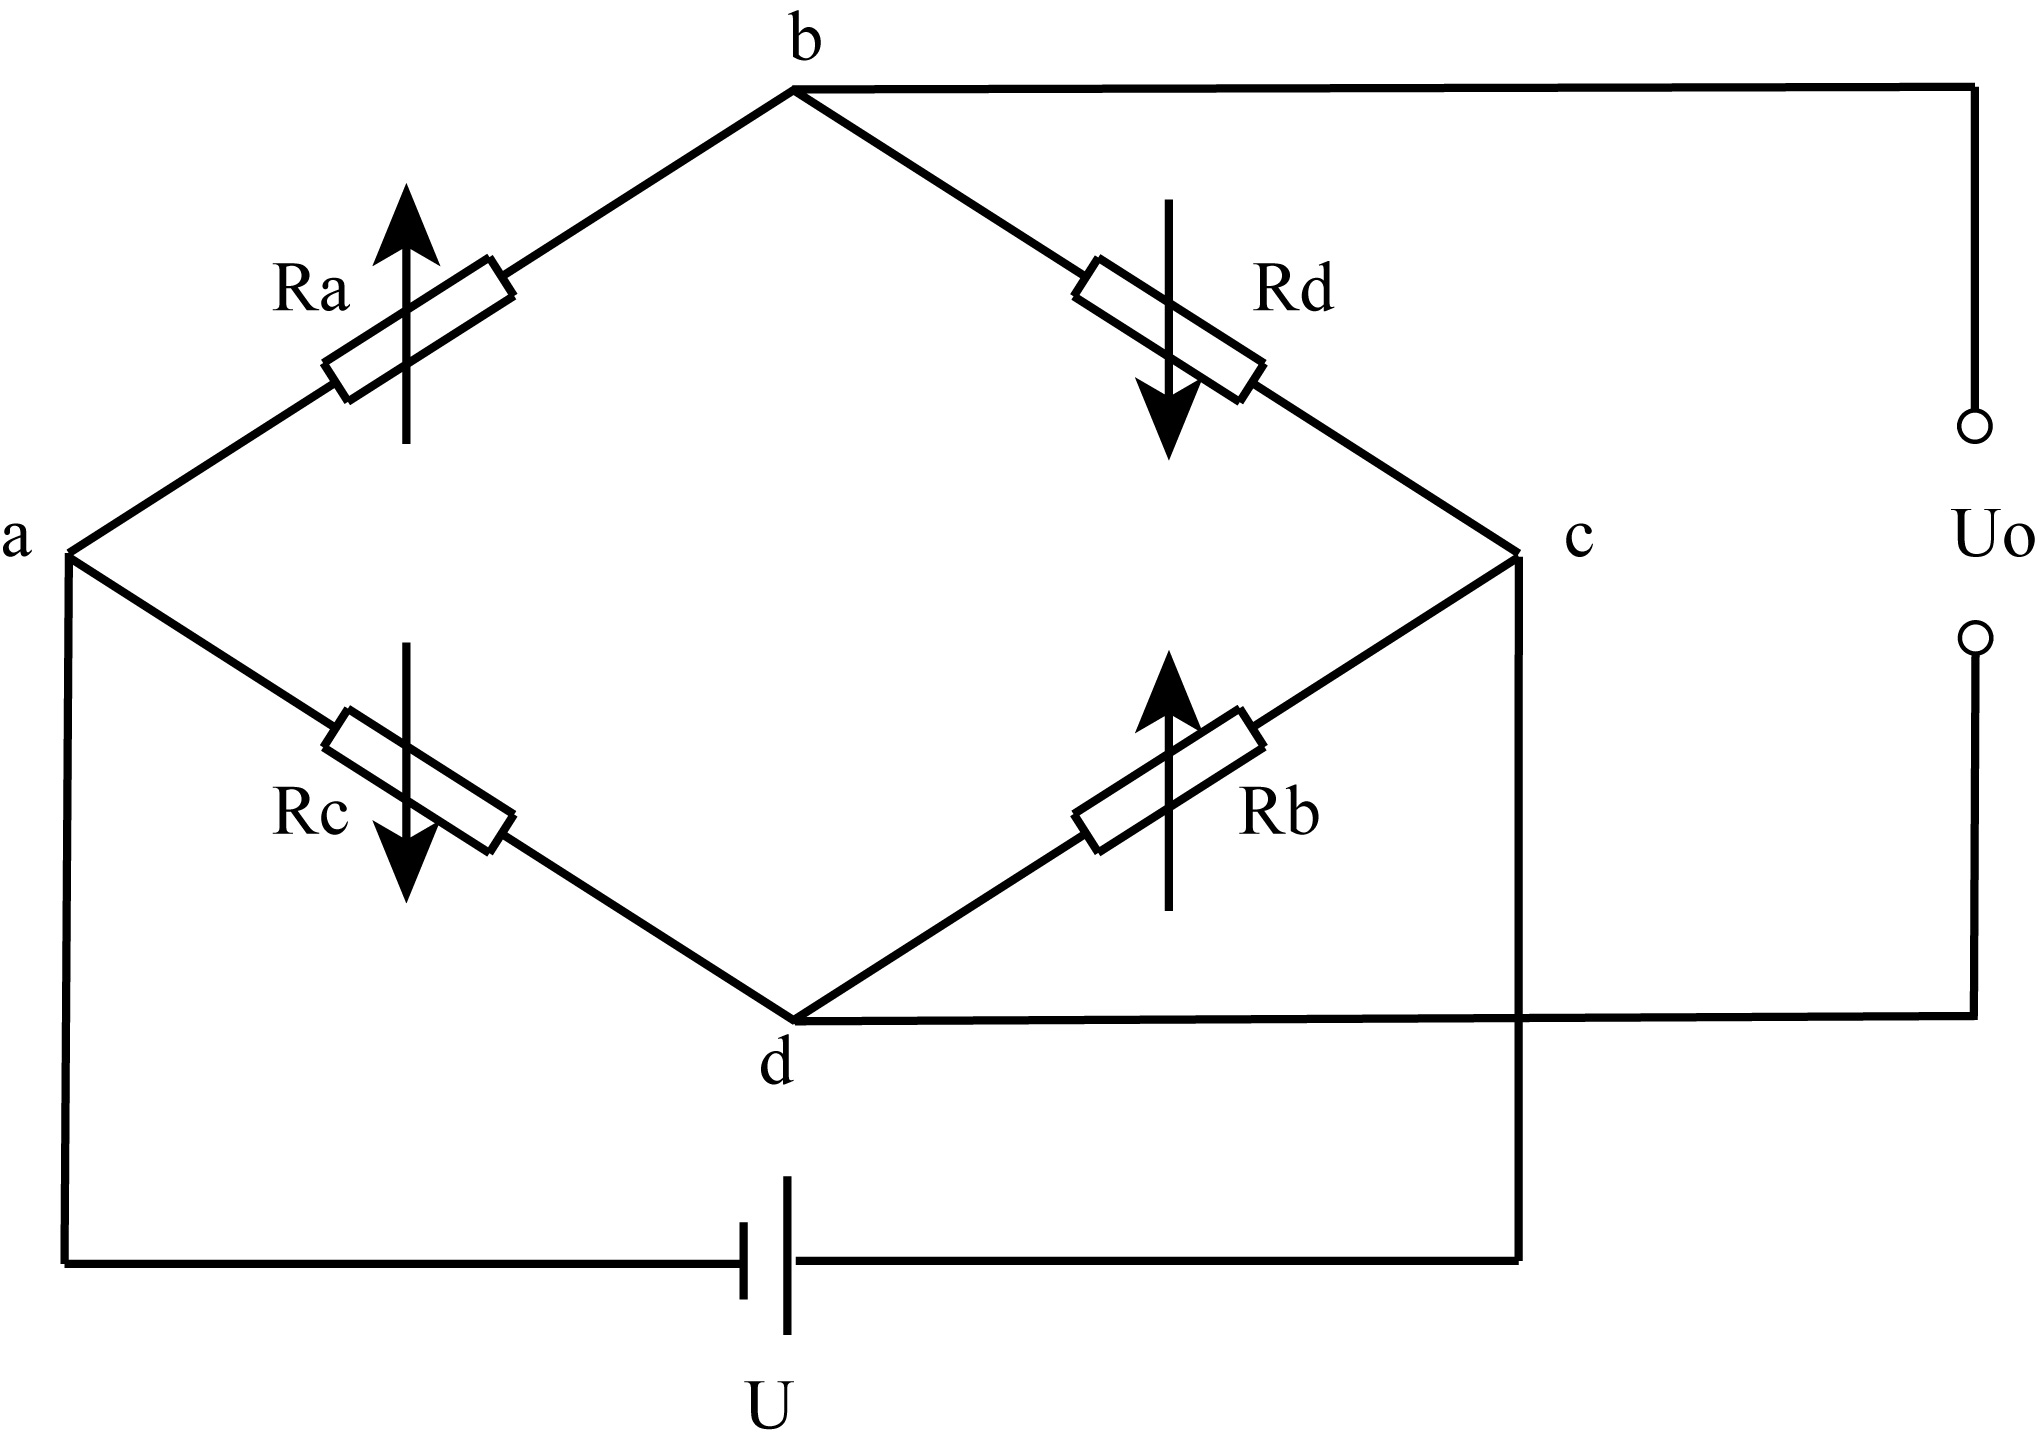
\includegraphics[width=8cm]{fig/f25.jpg}
    \caption{差动全桥应变测量电路}
    \label{fig:mark}
\end{figure}

这里使用差动全桥对应变进行测量,由如图2.5电路可得:
\begin{align}
U_o = U\cdot \frac{(R_a + \Delta R_a)(R_b + \Delta R_b) - (R_c - \Delta R_c)(R_d - \Delta R_d)}{(R_a + \Delta R_a + R_d - \Delta R_d)(R_b + \Delta R_b + R_c - \Delta R_c)}
\end{align}

设$R_a = R_b = R_c = R_d$,则:
\begin{align}
U_o = U\cdot \frac{\Delta R_a R_b + \Delta R_b R_a + \Delta R_c R_d + \Delta R_d R_c}{(R_a + R_d)(R_b + R_c)}= U\cdot \frac{\Delta R_a}{R_a}
\end{align}

选型上,项目中采用OMEGA公司的KFH-6-350-C1-11L1M2R的电阻应变片,使用FUTEK-IAA100放大器对全桥电路信号进行测量和放大,之后通过MicroLabBox的模拟量输入接口进行读取,并用于后续的力矩反馈控制。

\section{步态分析与步态周期测量}
\subsection{人体下肢运动步态分析}

为了能够对穿戴者提供有益的辅助作用,需要要对人体行走过程进行加以分析。步态周期是人体基本的运动之一,它定义为连续发生两次重复的步行事件之间的时间间隔。虽然可以选择任何事件来定义步态循环,但通常使用一只脚接触地面的瞬间(初始接触)作为开始。如果决定从右脚的初始着地开始,则到右脚再次接触地面为止,并如此循环。

\begin{figure}[htb]
    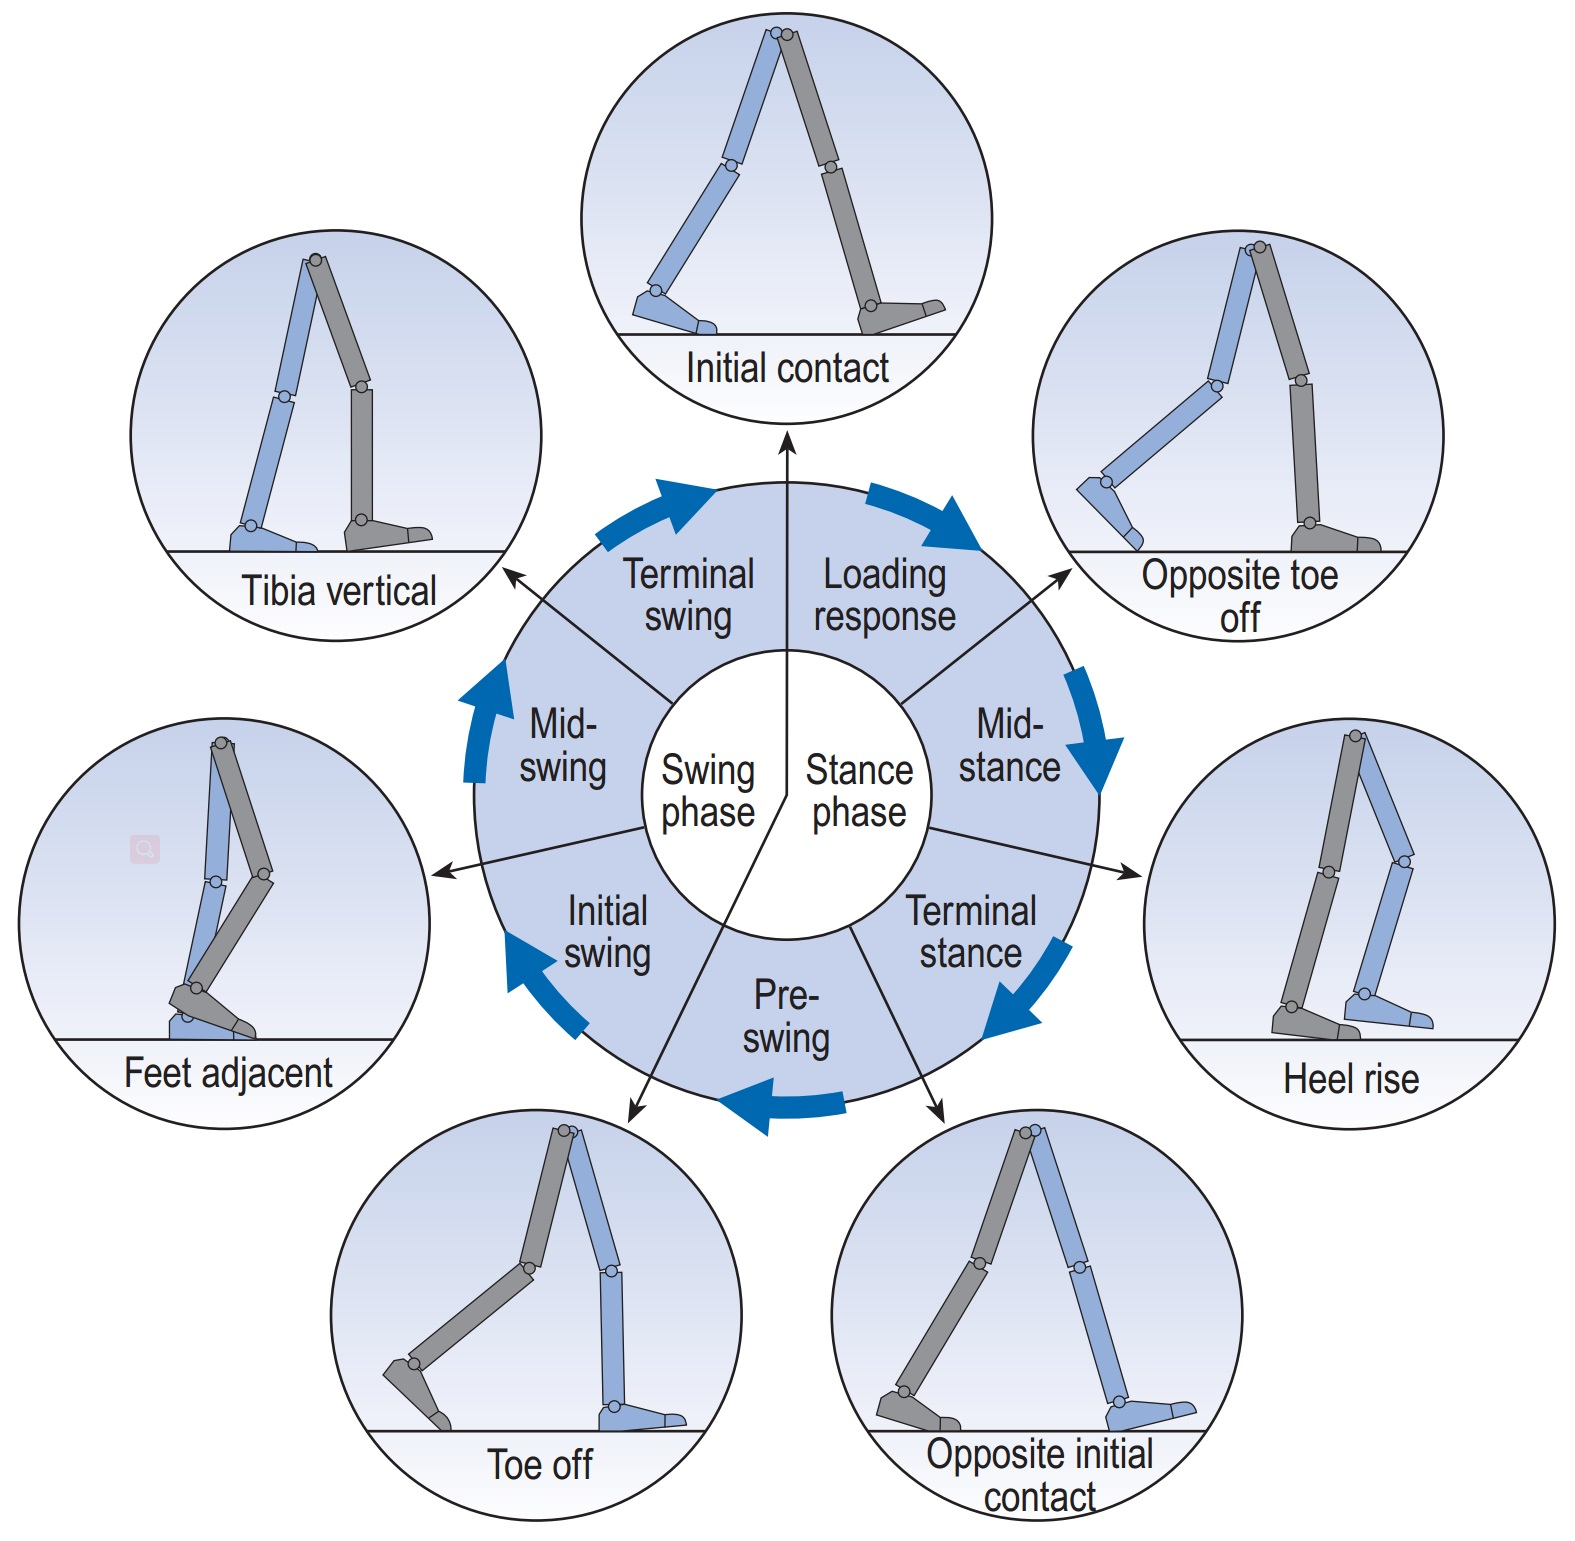
\includegraphics[width=14cm]{fig/f29.jpg}
    \caption{步态周期经历的过程}
    \label{fig:mark}
\end{figure}

如图2.7所示,在步态分析的教材\cite{p44}中,一般以7个术语件来定义步态周期的主要事件:
\begin{enumerate}
    \item 初始着地(Initial contact, IC)
    \item 反向脚趾离地(Opposite toe off, OT)
    \item 脚跟抬起(Heel rise, HR)
    \item 反侧初始着地(Opposite initial contact, OI)
    \item 脚趾离地(Toe off, TO)
    \item 双脚靠近(Feet adjacent, FA)
    \item 胫骨垂直(Tibia vertical, TV)
\end{enumerate}

这七个事件将步态循环分为7个阶段,其中4个阶段发生在脚着地时的站立相,3个阶段发生在脚在空中向前移动时的摆动相。站立相从初始着地一直持续到脚趾离地,并分为以下四个部分:
\begin{enumerate}
    \item 支撑初期(Loading response)
    \item 支撑中期(Mid-stance)
    \item 支撑末期(Terminal stance)
    \item 预摆动(Pre-swing)
\end{enumerate}

摆动相从脚趾离地开始持续到到下一次的初始着地。它又细分为:
\begin{enumerate}
    \item 摆动初期(Initial swing)
    \item 摆动中期(Mid-swing)
    \item 摆动末期(Terminal swing)
\end{enumerate}

\begin{figure}[htb]
    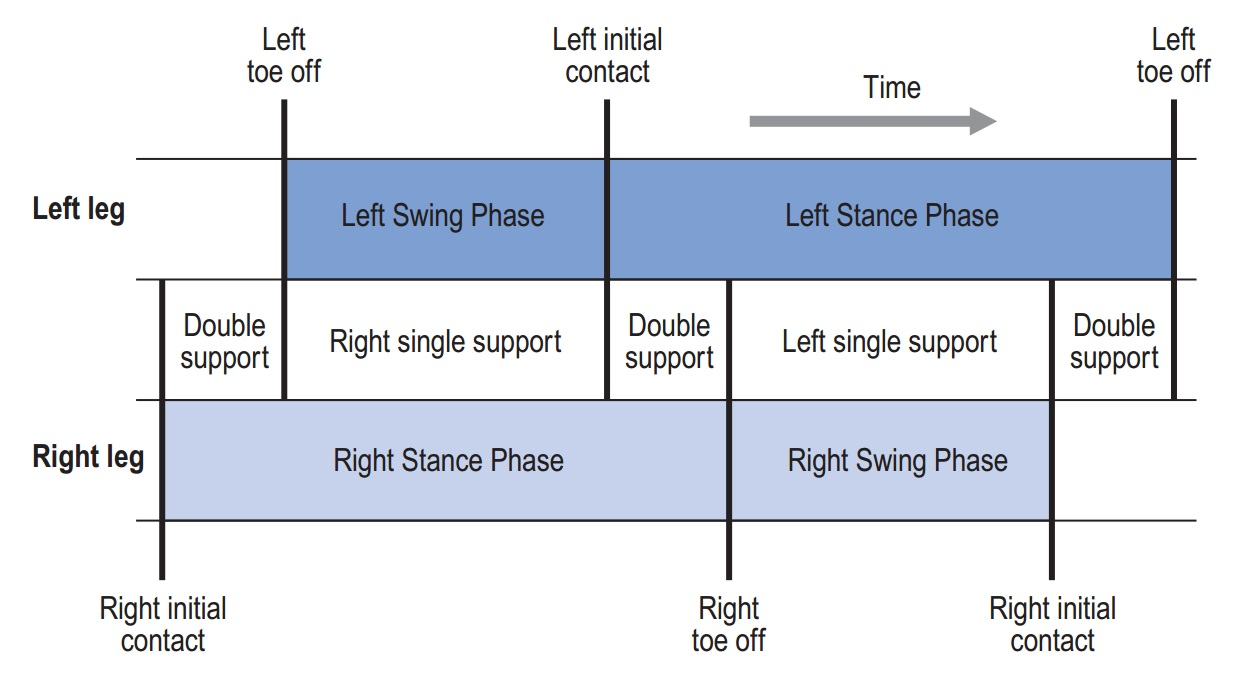
\includegraphics[width=15cm]{fig/f30.jpg}
    \caption{步态周期的时序}
    \label{fig:mark}
\end{figure}

图2.8显示了在一个多步态周期内,两只脚初始着地和脚趾离地的时间。当左脚还在地面上时,右脚开始接触地面,在右脚开始接触和左脚脚趾离开之间有一段时间的双支撑。在左腿摆动期间,只有右脚着地,右脚单支撑一段时间,并以左脚初始着地地面结束。然后是另一段双支撑期,直到右脚脚趾离地。左脚单支撑对应于右摆动相,周期结束时,下一个初始着地点在右侧。

因此,在每个步态周期中,有两个双支撑周期和两个单支撑周期。支撑相通常持续约60\%的周期,摆动相约40\%,每一阶段的双支撑约10\%。然而,这是随着行走速度的增加而变化的,随着速度的增加,摆动相成比例地变长,站立相和双支撑变短。双支撑阶段的消失也标志着从步行转变为跑步。

\subsection{基于足底开关的步态周期测量}

本文第三章在进行外骨骼力矩控制时,施加的力矩曲线与步态周期百分比具有密切关系。为了做到外骨骼控制与人体运动的同步,必须对步态周期进行准确的测量。常用的有使用足底开关、足底压力、关节角度等方法,本文采用简单且可靠的足底开关。

\begin{figure}[htb]
    \subfloat[足底开关]{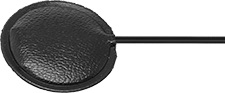
\includegraphics[width=6cm]{fig/f31.jpg}}\quad
    \subfloat[步态检测状态机]{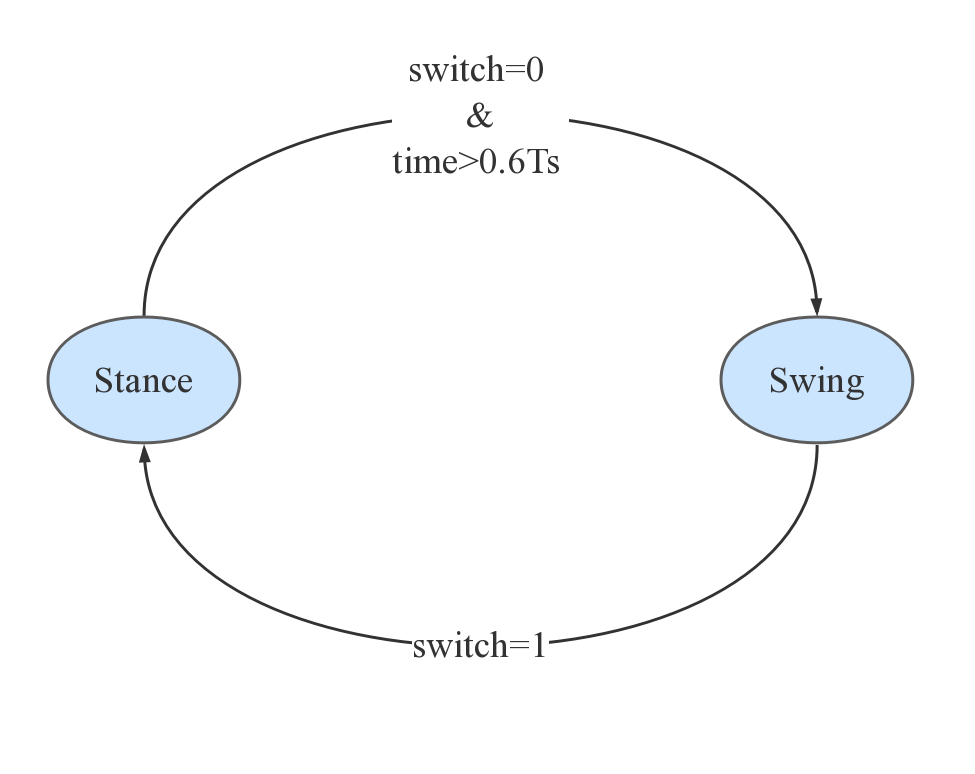
\includegraphics[width=8cm]{fig/f32.jpg}}
    \caption{足底开关与步态检测状态机}
    \label{fig:subfigss}
\end{figure}

如图2.9 a)所示的薄膜式接触开关被粘贴在外骨骼鞋子内部脚跟处,用以测量步态周期。传感器的两端连接到MicroLabBox的数字引脚上,一端配置为高电平的数字输出,另一端配置为下拉状态的数字输入。当足底开关所在腿处于摆动阶段时,开关处于断开状态,输入信号为低电平;当其切换到支撑阶段时,开关连通使输入信号变为高电平。由此可以对摆动相和支撑相进行检测,每次摆动相切换到支撑相时,便进入到一个新的步态循环,两个上升沿之间的时间便为一个步态周期的时间。

在实验中使用足底开关进行测量时会出现毛刺现象,因此单纯通过采集信号的高低电平来判断相位变化不甚可靠。为此本文提出一种步态检测状态机,如图2.9 b)所示,摆动相转换支撑相时,只通过高电平判断,这样可以准确测量到步态周期的开始时刻。在支撑相转换到摆动相时,除了电平还要做一个时间检测,只有在当前步的时间大于前一步完整步态周期时间的60\%时,才由支撑相转换到摆动相。通过此方法可以准确检测摆动-支撑的转换,同时可以有效的消除信号毛刺,但无法检测出支撑-摆动的转换,此转换根据人体步态过程的统计规律得到。

\begin{figure}[htb]
    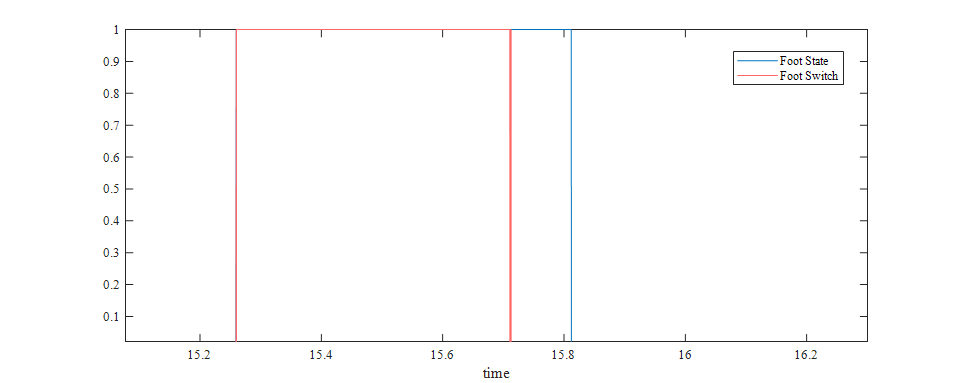
\includegraphics[width=16cm]{fig/f33.png}
    \caption{足底开关信号与步态检测}
    \label{fig:mark}
\end{figure}

\section{IMU原理}
\subsection{IMU原理与Kalman滤波}
IMU即惯性测量单元,它可以测量得到物体的加速度和角速度信息。IMU可以根据自由度(DoF)的不同分为不同的类型,6DoF的IMU中包含三轴加速度计和三轴陀螺仪。三轴加速度计能够测量三个方向上加速度的大小,三轴陀螺仪能够测量三个轴角速度的大小,如图中2.11(a)所示。

\begin{figure}[htb]
    \subfloat[IMU]{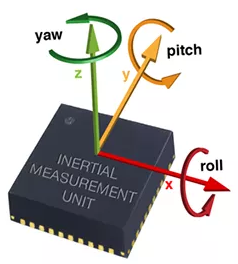
\includegraphics[width=3.5cm]{fig/f34.png}}
    \subfloat[加速度计]{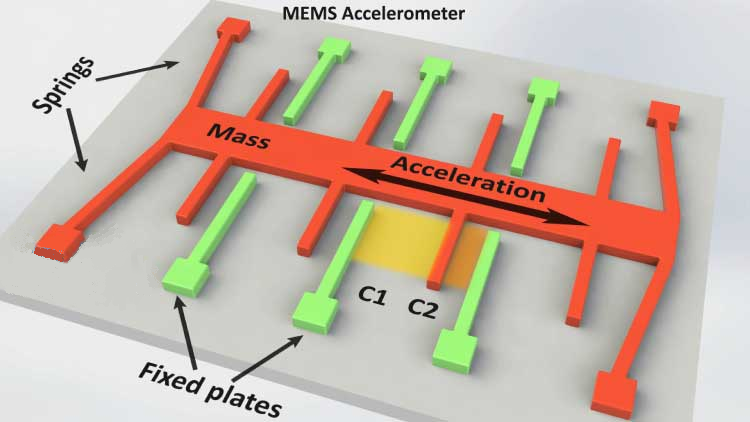
\includegraphics[width=6.5cm]{fig/f35.png}}
    \subfloat[陀螺仪]{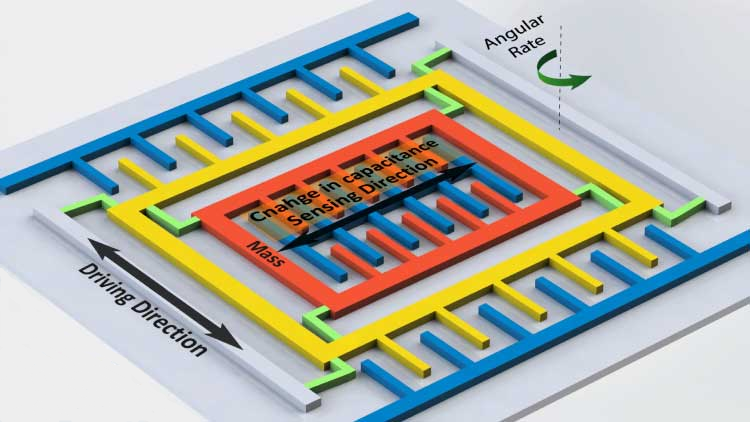
\includegraphics[width=6.5cm]{fig/f36.png}}
    \caption{IMU与其内部构成}
    \label{fig:subfigss}
\end{figure}

加速度的测量利用了牛顿第二定律。如图2.11(b)所示,中间红色的为一个质量块,两头通过具有弹簧性质的杆状结构与基底相连,红色的短栅与绿色的短栅分别为电容的极板。当传感器在箭头方向受到加速度$a$时,由于质量块与基底相连因而有相同的加速度,这个加速度的由弹簧产生,根据$f=ma=kx$,质量块会沿加速度相反的方向移动一定距离,即红色极板与绿色极板之间的距离会发生变化。通过测量极板电容C的变化就可以得到加速度的大小。在三轴加速度计中,这样的结构在三个方向各有一个,且做到了微米的尺寸,并配合相应的测量电路集成在一个芯片中,构成一个微机电系统(MEMS)。

角速度测量的原理比加速度要复杂一些,它利用了科里奥里力(Coriolis Force)。当物体在旋转的坐标系下运动时,由于坐标系的旋转会在垂直其运动方向上受到一个作用力,即科里奥里力,$F=-2mvω$。科里奥里力是由坐标系的转动与物体在动坐标系中的相对运动引起的,其本质是物体的惯性。

陀螺仪的物理实现如图2.11 c)所示,外侧的蓝色与黄色部分为驱动电极,内部的红色与蓝色为测量电极。首先在模块的驱动方向施加正弦驱动电压,使模块沿驱动方向做正弦运动。当模块发生旋转时,质量块受科里奥里力影响在测量方向会发生运动,而且是正弦运动,且正弦运动的幅值与角速度成正比,通过电极测量出此幅值,便可以得到模块角速度。与三轴加速度计一样,这样的结构在三轴陀螺仪的三个方向上各有一个,从而测量出三个方向的角速度。

\subsection{IMU姿态解算与数据融合}

\begin{figure}[htb]
    \subfloat[IMU水平放置]{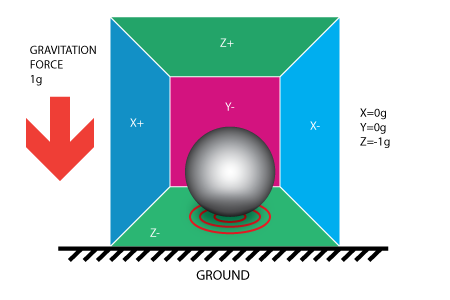
\includegraphics[width=8cm]{fig/f37.png}}\quad
    \subfloat[IMU倾斜放置]{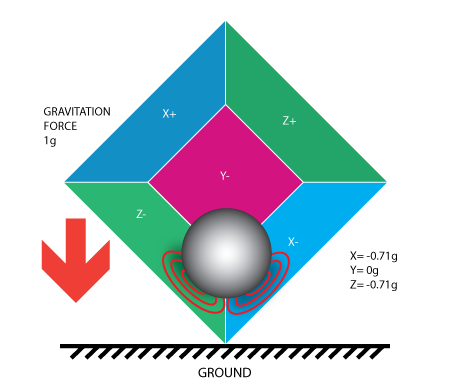
\includegraphics[width=7cm]{fig/f38.png}}
    \caption{通过加速度计解算角度信息}
    \label{fig:subfigss}
\end{figure}

加速度计和陀螺仪都无法直接得到角度数据,需要从加速度和角速度解算出角度信息。可以把加速度计中的质量块当做左图中的小球,由加速度计的原理可知,在传感器静止的时候,测量的结果为重力加速度,因此当传感器倾斜时,如右图所示,可以根据重力加速的在三轴分量的大小来解算出角度:
\begin{align}
Angle_{Accel} = arccos\frac{ax}{-g}
\end{align}
从角速度解算出角度更简单,只需要知道初始角度然后对角速度进行积分就可以了:
\begin{align}
Angle_{Gyro}=Angle_0 + \int_0^t Gyro dt
\end{align}
本文分析的仅为单轴的情况,对于三轴角度解算还需要涉及坐标系转换。

通过加速度和角速度都可以解算出角度信息,但这两种方式都存在很大的问题。加速度计由于容易受到振动的影响,噪声很大,所以解算出角度的噪声也很大;通过角速度积分得到角度的方式,由于初始角度并不能准确得到,而且角速度存在零偏和零漂问题,偏移误差会被累积导致角度不断漂移。因此,两种方式解算出来的角度都无法直接使用。

接下来采用Kalman滤波的方法,把两个传感器的数据融合在一起,得到一个既没有累计误差、噪声又小的角度信息。首先建立Kalman滤波器的状态观测方程。本文选择需要观测的角度$\theta$和陀螺仪角速度偏置$\omega_b$作为状态变量,陀螺仪的角速度为控制变量,加速度计解算得到的角度$\theta_{accel}$作为观测变量,并由此得到状态空间方程:

\begin{align}
\begin{bmatrix} \theta(k+1)  \\ \omega_b(k+1)   \end{bmatrix} &= \begin{bmatrix} 1 & -dt \\ 0 & 1   \end{bmatrix}\begin{bmatrix} \theta(k)  \\ \omega_b(k) \end{bmatrix} + \begin{bmatrix} dt \\ 0  \end{bmatrix} \omega(k) \\
\theta_{accel}(k) &=\begin{bmatrix} 1 & 0  \end{bmatrix}  \begin{bmatrix} \theta(k) \\ \omega_b(k)  \end{bmatrix}
\end{align}
其中式2.5为公式2.4的推广,式2.6中的$\theta_{accel}$由式2.3计算得到。之后令:
\begin{align}
X(k) = \begin{bmatrix} \theta(k)  \\ \omega_{b}(k) \\  \end{bmatrix}, \quad U(k) = \omega(k), \quad Y(k) = \theta_{accel}(k)
\end{align}
并将状态空间方程表示成如下标准形式:
\begin{align}
X(k+1) &= A X(k) + B U(k) + G W(k) \\
Y(k) &= C X(k) + V(k)
\end{align}

式中$W(k)$为输入白噪声,反应系统建模的不准确性;而$V(k)$表示观测噪声,反应传感器信号采集时的干扰噪声。

对于上面建立的状态空间方程,使用卡尔曼滤波器进行滤波。Kalman滤波方程组由五个方程组成:
\begin{align}
    状态一步预测: & \hat{X}(k+1|k) = A \hat{X}(k|k) + B U(k) \\
    状态更新:& \hat{X}(k+1|k+1) = A \hat{X}(k+1|k) + K(k+1)[Y(k+1)-C\hat{X}(k+1|k)] \\
    增益矩阵更新:& K(k+1) = P(k+1|k)C^T[CP(k+1|k)C^T + R]^{-1} \\
    协方差矩阵一步预测:& P(k+1|k) = AP(k|k)A^T+GQG^T \\
    协方更新:& P(k+1|k+1) = [I_n-K(k+1)C]P(k+1|k)
\end{align}

在实际使用时,需要为滤波器设置合适的状态初始值和协方差矩阵初始参数。同时需要适当调整方差阵$Q$和$R$的参数,方能得到较好的滤波效果。对于本文所建立的模型而言,观测噪声远大于模型噪声,因此方差阵$R$中的参数比$Q$要大一些。

\subsection{姿态采集系统设计}


\begin{figure}[htb]
    \label{fig:sub1}{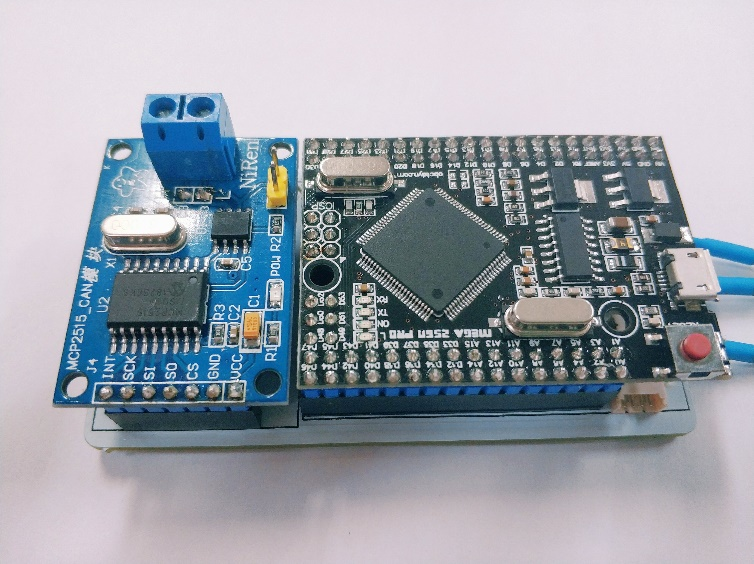
\includegraphics[width=7cm]{fig/f40.jpg}}\quad
    \label{fig:sub2}{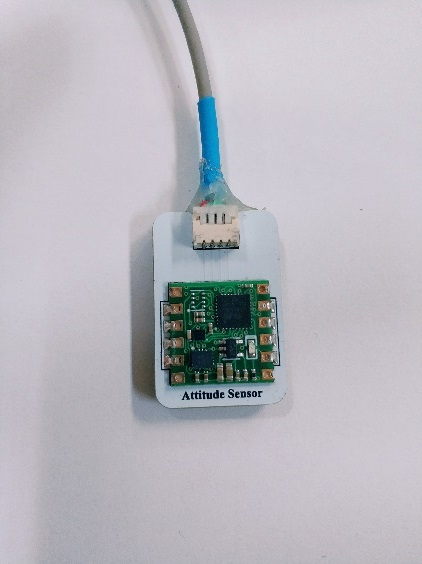
\includegraphics[width=4cm]{fig/f41.jpg}}
    \caption{基于IMU的姿态采集系统}
    \label{fig:subfigss}
\end{figure}

\begin{figure}[!h]
    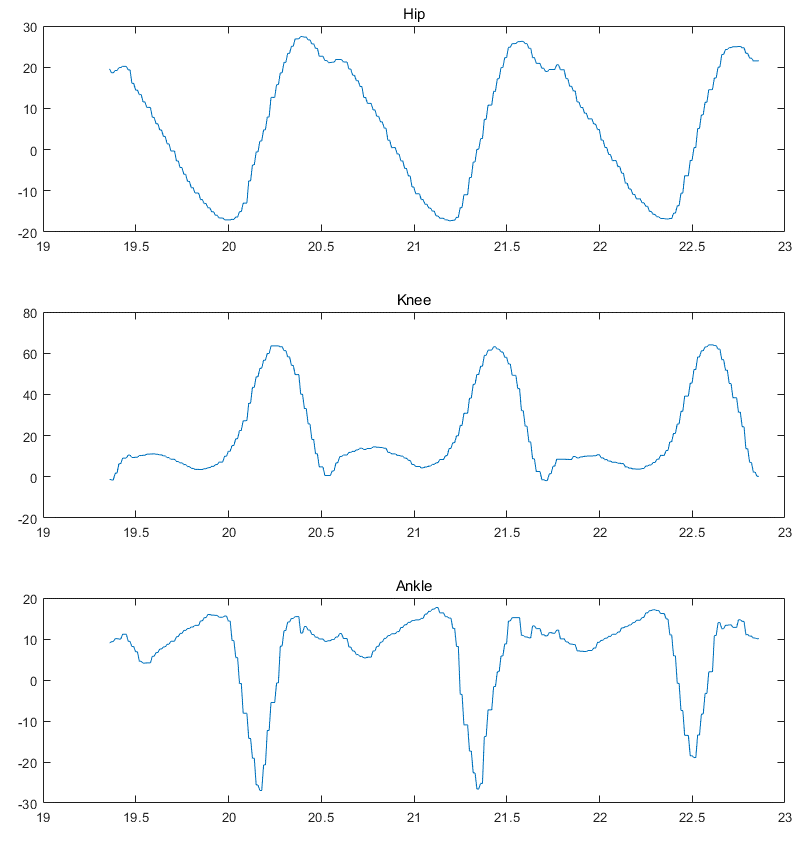
\includegraphics[width=13.5cm]{fig/f39.png}
    \caption{姿态采集系统得到的关节角度曲线}
    \label{fig:mark}
\end{figure}

为了测量人体的运动学数据,本文设计基于IMU的姿态测量系统,如图2.13所示,左图所示的为单个IMU模块,它可以被安装在身体的各个部分;右图为是数据采集与处理模块,它通过I2C总线连接三个IMU模块,通过Kalman滤波解算三个模块的姿态角度,之后将姿态角转换为人体的关节角度,并通过CAN总线发送给MicroLabBox。通过本文设计的姿态采集系统得到的关节角度曲线如图2.14所示。

\section{肌电信号采集与处理}
\subsection{肌电信号原理}
\begin{figure}[htb]
    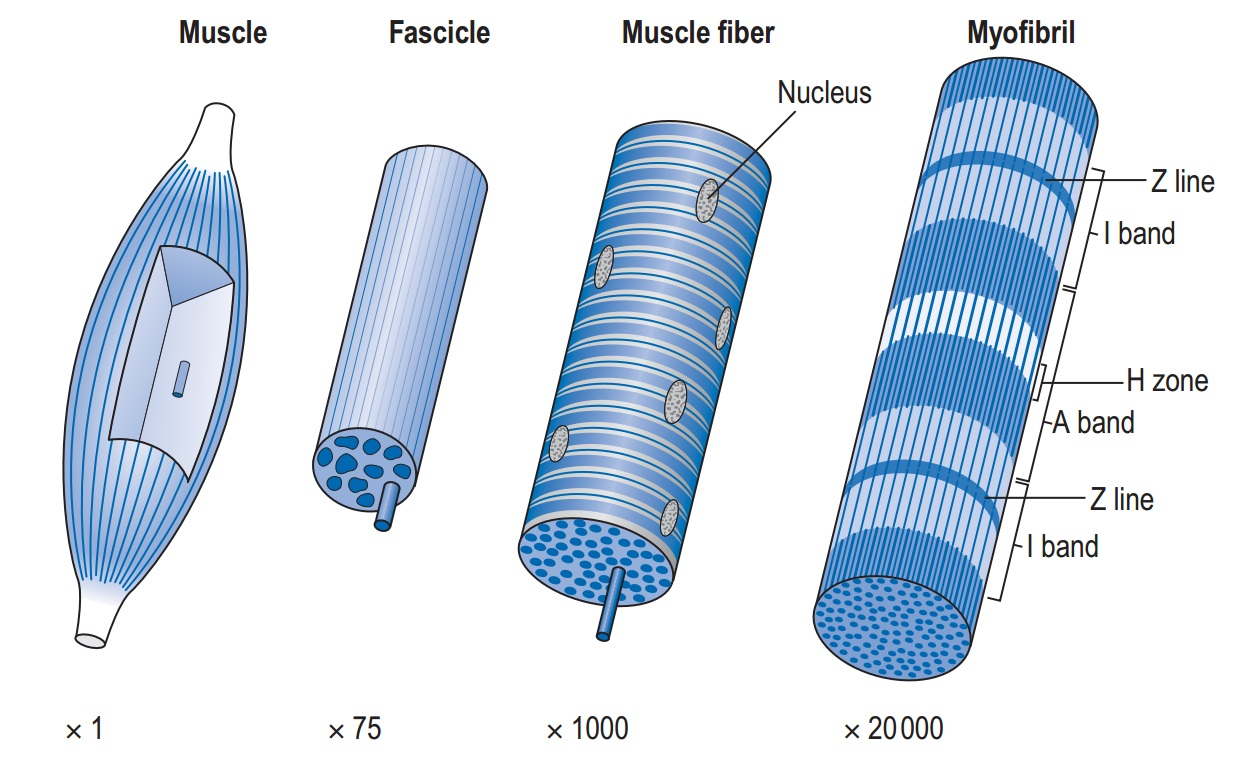
\includegraphics[width=14cm]{fig/f43.jpg}
    \caption{人体肌肉机结构示意图\cite{p44}}
    \label{fig:mark}
\end{figure}
人体有三种肌肉:平滑肌、心肌和骨骼肌,其中负责四肢的运动主要为骨骼肌。肌肉由数百个束组成,如图2.15,而每个束又由数百个肌纤维组成。肌纤维是肌肉组织的基本单位,其本身是由数百个肌原纤维组成的。这些肌原纤维具有典型的条纹状外观,条纹是由两种蛋白质——肌动蛋白和肌球蛋白——构成的有规则排列的丝状物,正是这些纤维通过桥的形成和破坏相互滑动导致肌肉收缩。在肌肉纤维的外面是毛细血管和运动神经的末端分支,它们在运动终端(神经肌肉接头)与肌肉纤维连接。平均一条运动神经会连接到大约150条肌纤维,神经元和它所支配的肌纤维的组合被称为运动单元。

\begin{figure}[htb]
    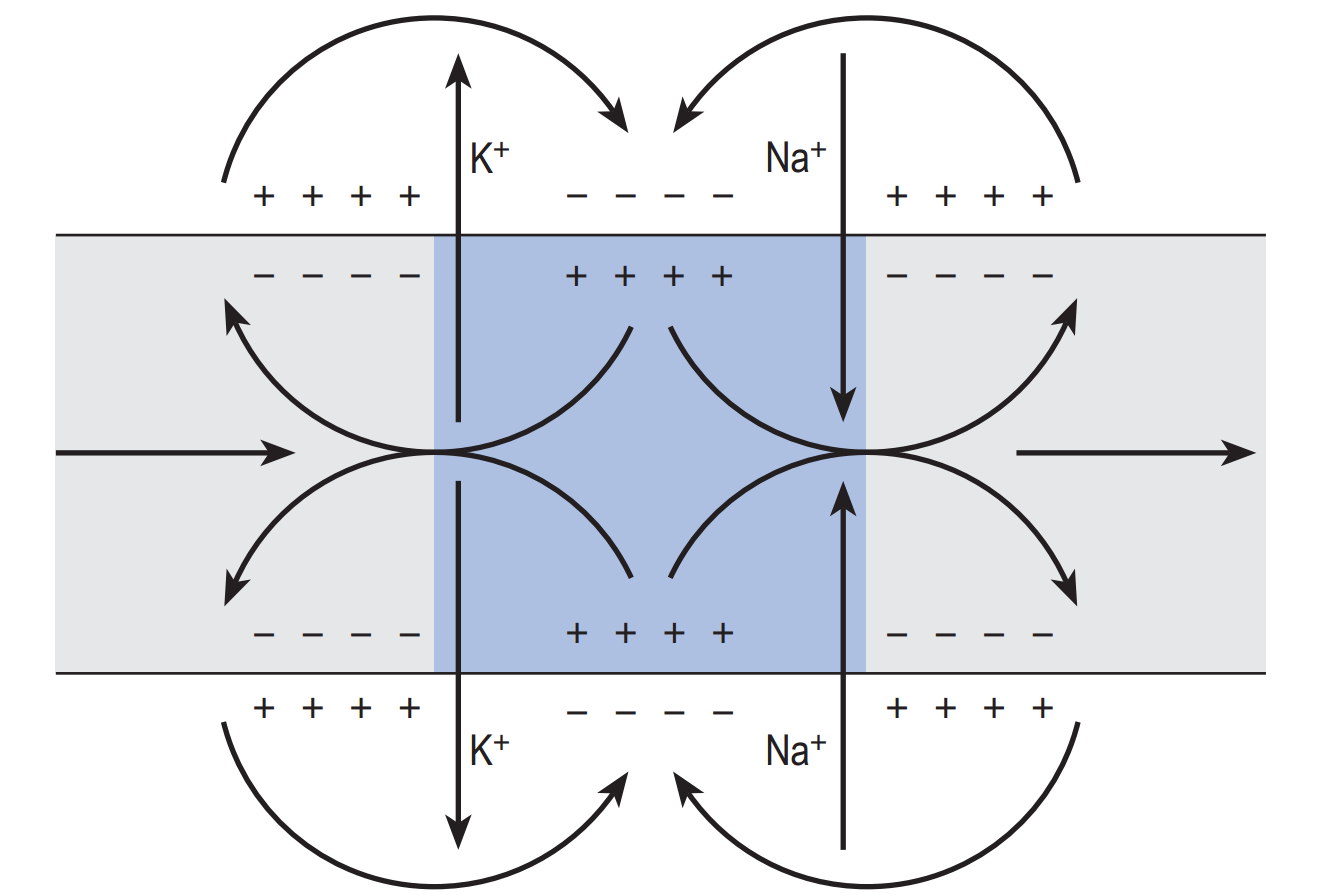
\includegraphics[width=10cm]{fig/f42.png}
    \caption{细胞动作电位示意图\cite{p44}}
    \label{fig:mark}
\end{figure}

当动作电位通过神经传递到运动终端时,会导致传递物质乙酰胆碱的释放,使肌纤维的细胞膜去极化。当这种肌肉动作电位在肌肉纤维中扩散时,它会导致钙离子的释放,从而触发肌肉收缩。肌动蛋白和肌球蛋白分子之间形成了桥梁,将它们拉在一起,这种张力维持了很短的一段时间,如果没有进一步的动作电位发生,就释放出来,钙离子被钙泵移除。如图2.16所示,肌肉动作电位的电活动可以检测出来,称为肌电图(EMG)。

EMG信号是众多运动单元动作电位在时间和空间上的叠加,根据具体测量方式又可分为针电极信号NEMG和表面肌电信号sEMG。表面肌电信号是浅层肌肉和神经电活动在皮肤表面的综合效应,能在一定程度上反映出神经肌肉的活动;相对于NEMG,SEMG在测量上具有非侵入性、操作简单等优点,因此广泛应用于临床医学、体育科学等领域。

\subsection{sEMG信号的采集与处理}
\begin{figure}[htb]
    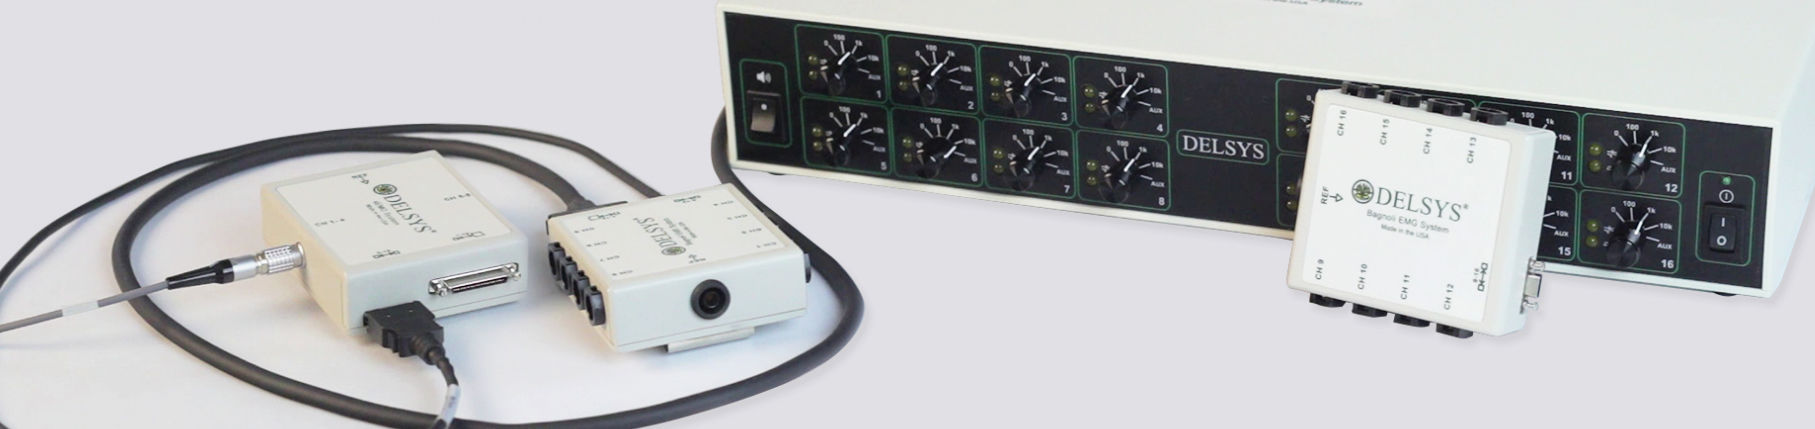
\includegraphics[width=16cm]{fig/f44.jpg}
    \caption{DELSYS 16通道EMG测量系统}
    \label{fig:mark}
\end{figure}
sEMG信号非常微弱,需要专用仪器进行采集。本文采用DELSYS公司生产的16通道EMG测量系统,可以实现16通道EMG数据的同时采集,采集的信号以模拟量形式连接到MicroLabBox的模拟量输入通道。以手臂的肱二头肌为例,采集的EMG如图2.18所示。

\begin{figure}[htb]
    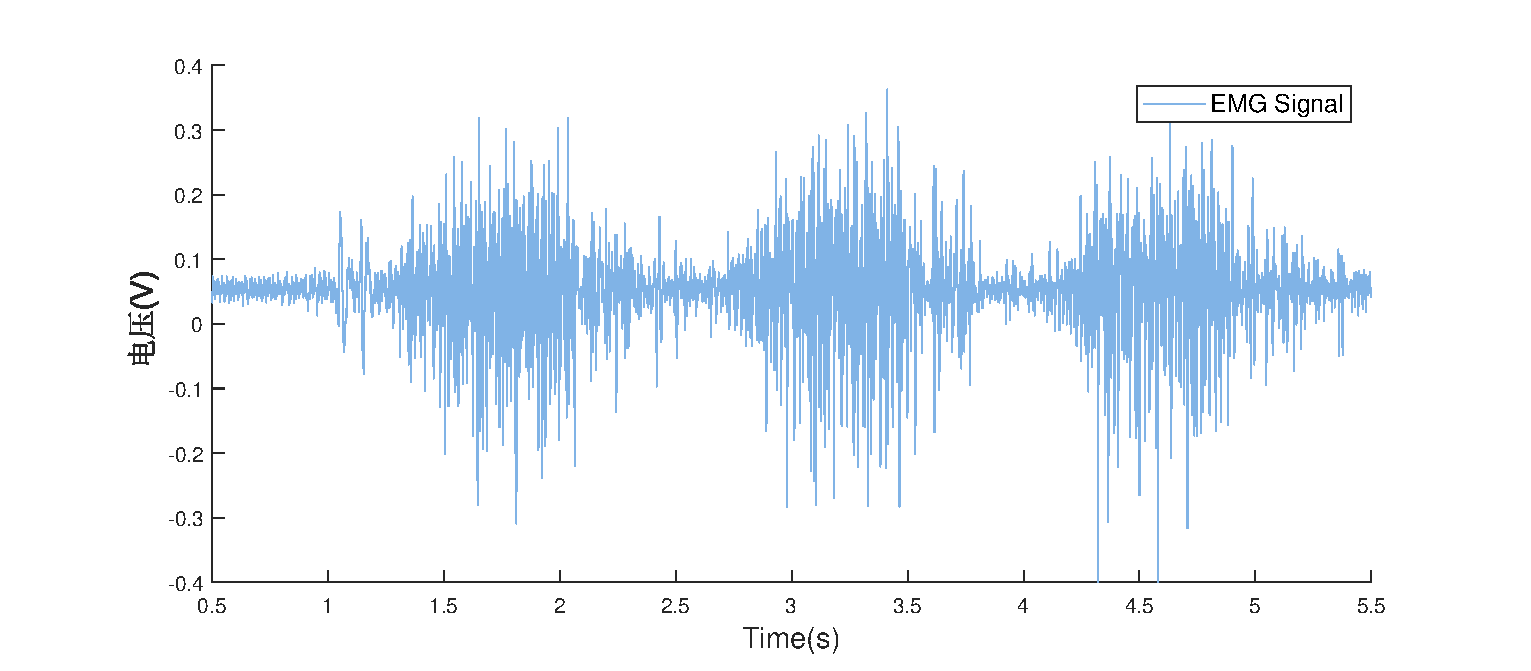
\includegraphics[width=17cm]{fig/f45.eps}
    \caption{肱二头肌收缩时的EMG信号}
    \label{fig:mark}
\end{figure}

\begin{figure}[htb]
    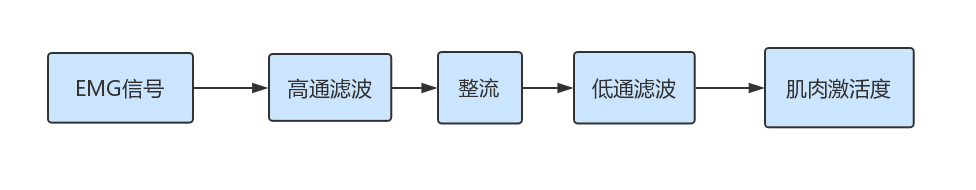
\includegraphics[width=16cm]{fig/f47.png}
    \caption{EMG信号处理流程}
    \label{fig:mark}
\end{figure}

\begin{figure}[!h]
    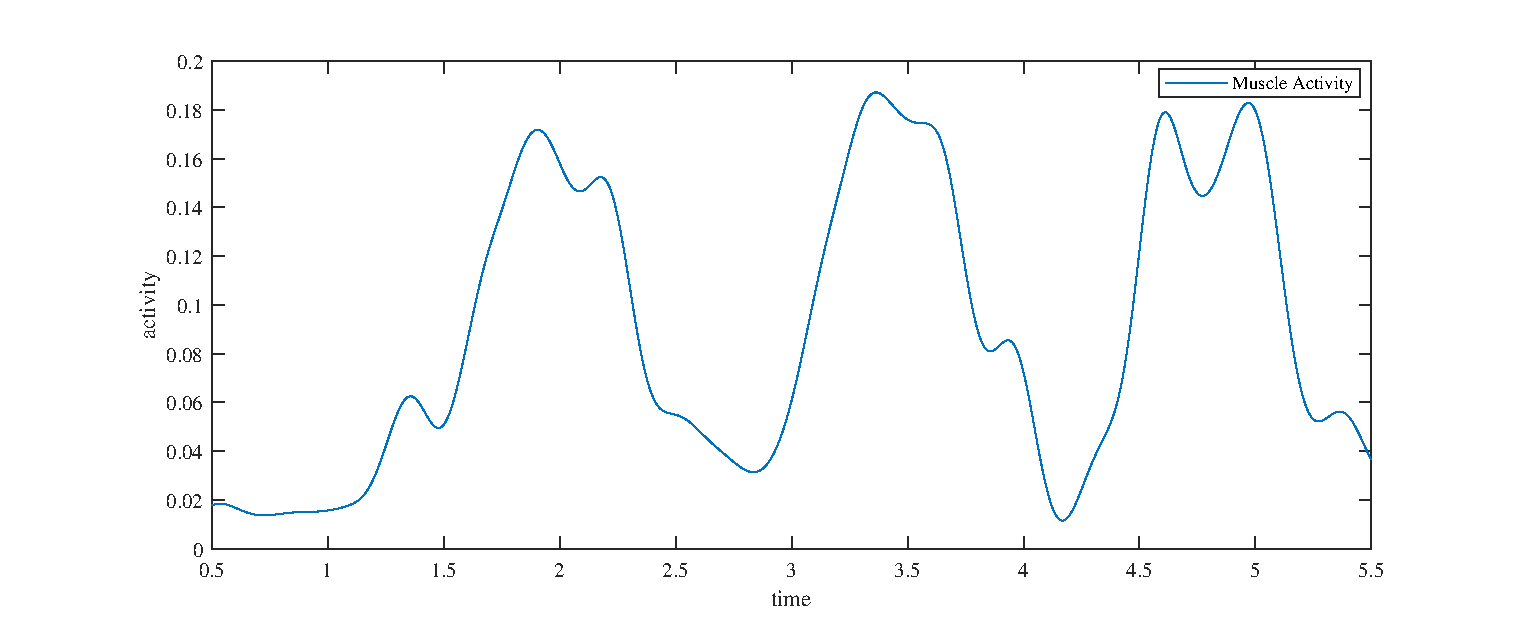
\includegraphics[width=17cm]{fig/f46.eps}
    \caption{肱二头肌收缩时的肌肉激活度曲线}
    \label{fig:mark}
\end{figure}

由于EMG信号是众多运动单元动作电位在时间和空间上的叠加,为典型的非平稳信号。生物学领域为从EMG信号中得到肌肉的激活的信息,较多的采用图2.19所示的方法对EMG进行滤波处理\cite{p45}。由于采集仪器和测量电路的影响,EMG信号中存在直流偏置,所以首先需要进行截止频率为25Hz高通滤波;之后对信号进行整流,再通过截止频率为4Hz的低通滤波器滤除高频分量,最终得到肌肉的激活信息。由图2.18 EMG信号滤波后的肌肉激活曲线如2.20所示。

\section{本章小结}

本章针对所研究的踝关节式外骨骼搭建了一套传感系统,搭建外骨骼力矩应变测量电路,使用足底开关检测人体的步态周期,设计了基于IMU的人体姿态数据采集系统,实现了基于EMG信号的肌肉激活度检测。除了上述部分外,该传感系统还包括测量电机角度的编码器、人体代谢数据的心肺呼吸仪和足底压力鞋垫等,但与本文后续内容无密切关系,故不再加以赘述。
\chapter{外骨骼力矩控制}

外骨骼机器人作为一个富有活力的课题已存在超过半个世纪,然而最适合此类系统的控制方法至今尚无定论。早期的外骨骼系统大多使用运动轨迹追踪的控制方法,但位移控制在人机动作不一致时会产生大的作用力,从而产生人机交互的安全风险。因此外骨骼控制正越来越多的从单纯的轨迹控制,转向对穿戴者动作反应更加柔和的力矩控制。

在实际的应用中,力矩控制一般由底层控制器和上层控制器组成。上层控制器(如阻抗控制器)用来产生期望的外骨骼力矩,而底层控制器(如PID控制器)用来控制驱动器对外骨骼期望的力矩进行追踪。在这种控制策略中,期望力矩并不是事先选定好的控制目标,而是由人机交互过程中产生的动态信号。典型的上层控制器有直接力矩控制\cite{p32,p33}、阻抗控制\cite{p34}、灵敏度放大控制\cite{p35}和基于EMG信号的控制方法\cite{p36},这些上层的控制策略均需要根据穿戴者的个体特性来对控制调整参数,以达到最佳的助力效果。底层控制器的形式较为多样,如经典的PID反馈控制\cite{p27,p28}、基于逆动力学模型的前馈力矩补偿\cite{p7,p22,p29}、自适应控制\cite{p30}、迭代学习\cite{p31}等。

\begin{figure}[!h]
    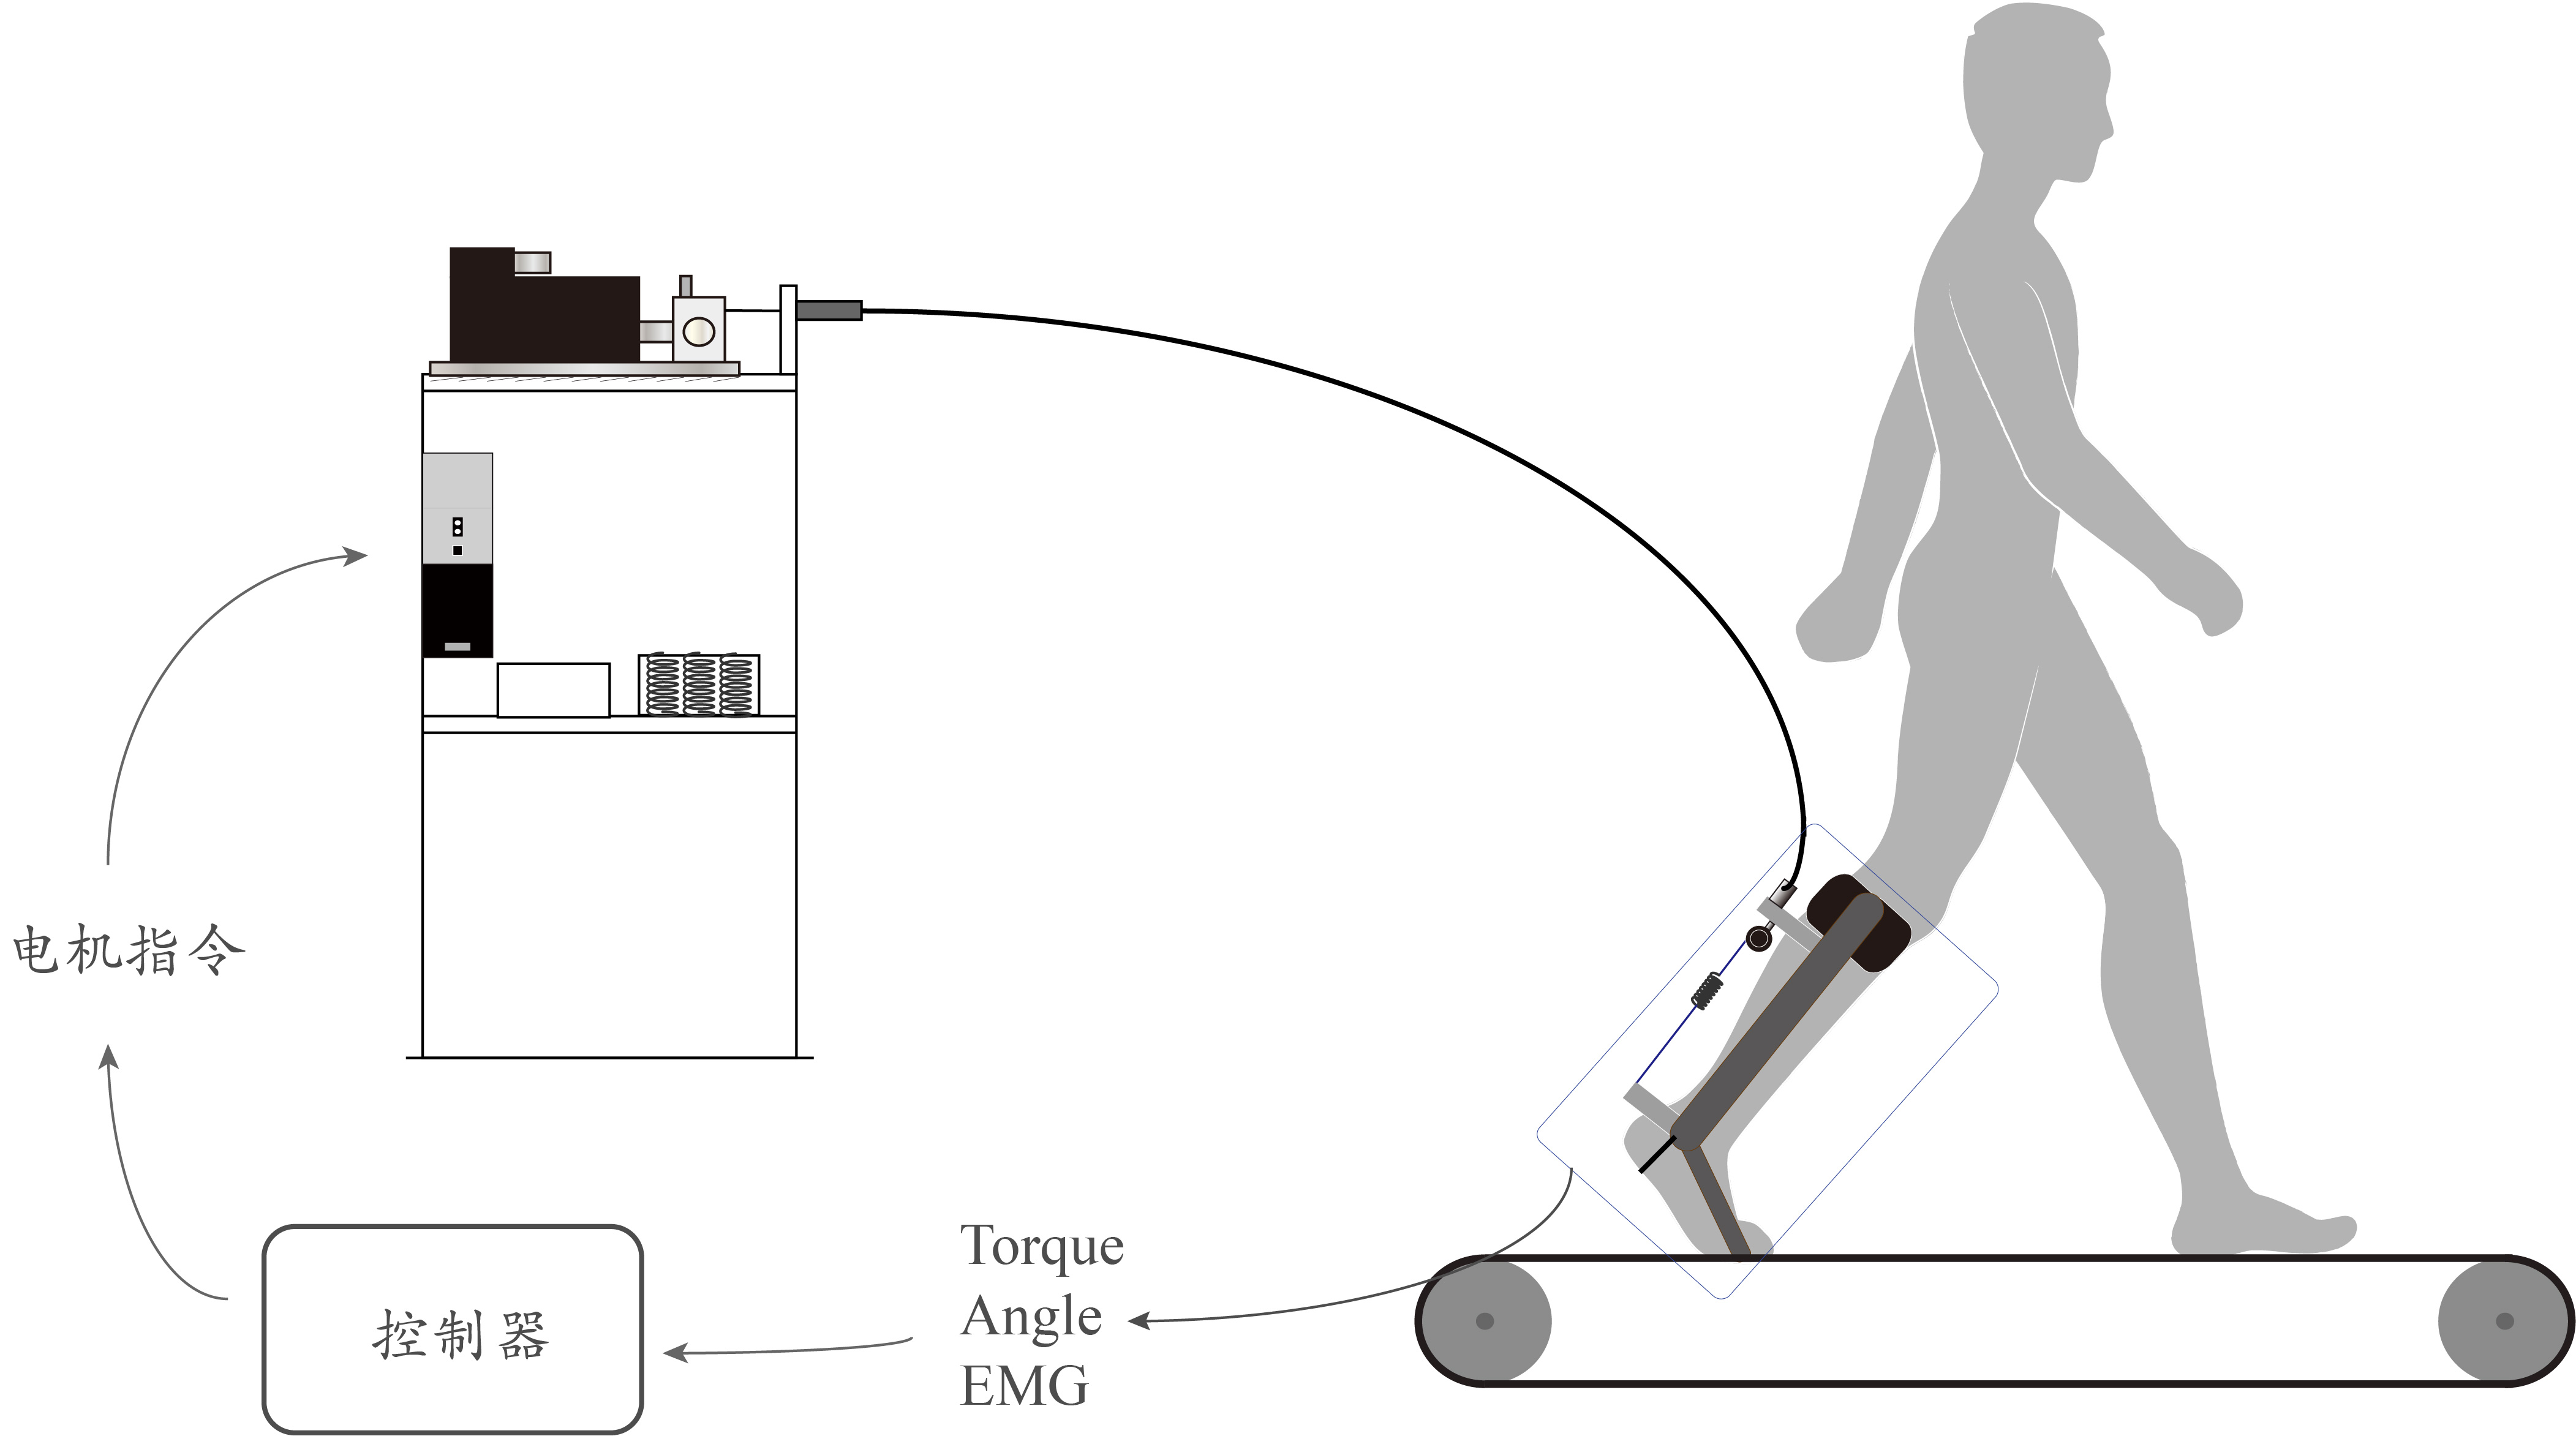
\includegraphics[width=15cm]{fig/f48.jpg}
    \caption{外骨骼力矩控制的硬件结构}
    \label{fig:mark}
\end{figure}

本章研究外骨骼的底层力矩跟踪控制算法。外骨骼力矩控制的硬件结构与组成如图3.1所示,受试者穿戴外骨骼在跑步机上以4.5Km/h的速度稳定的行走。通过第二章介绍的传感系统采集得到外骨骼和人体的相关数据送至dSPACE实时目标机,在dSPACE设计上层控制器产生期望力矩曲线,并搭建不同的底层力矩追踪控制算法产生电机控制指令,控制电机转动产生作用力,作用力通过鲍登线和串联弹簧作用到外骨骼上,为穿戴者提供力矩辅助。

\section{外骨骼系统动力学建模}

\begin{figure}[htb]
    \label{fig:sub1}{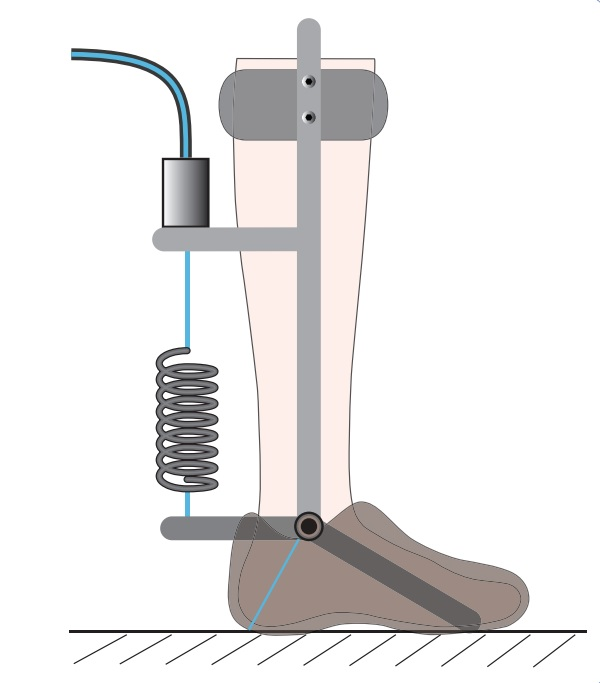
\includegraphics[width=7cm]{fig/f50.jpg}}
    \label{fig:sub2}{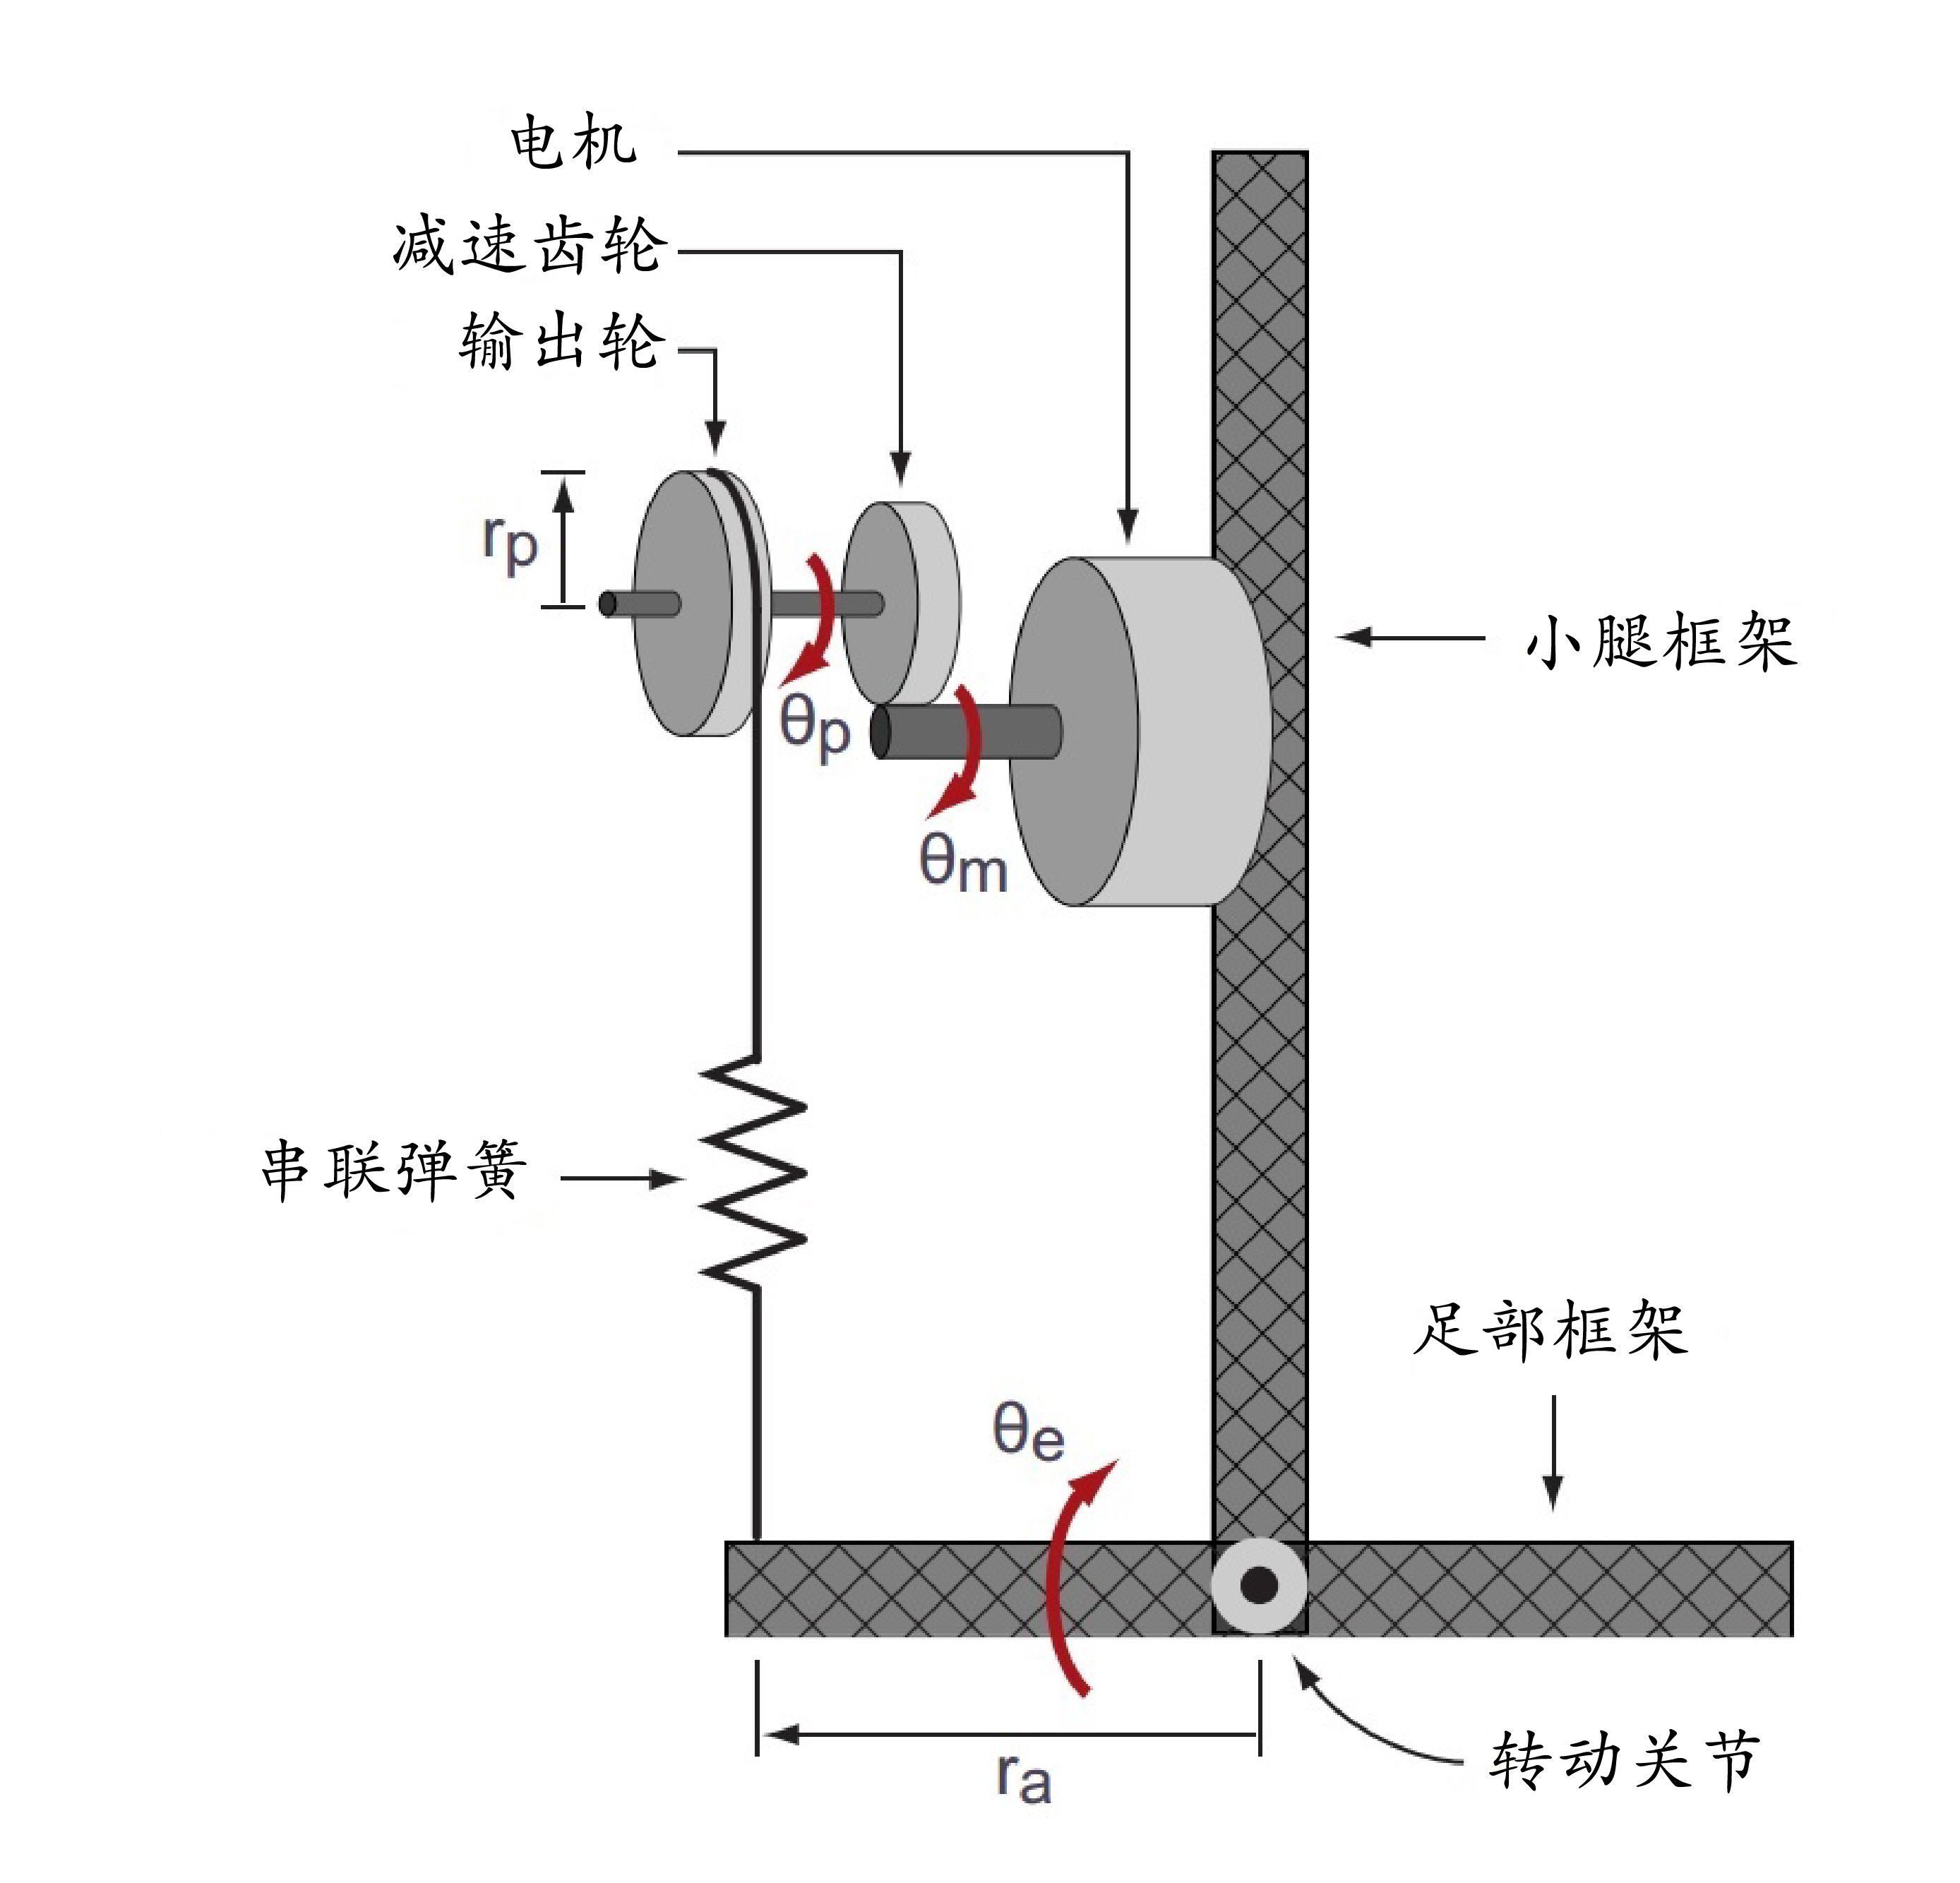
\includegraphics[width=9cm]{fig/f49.jpg}}
    \caption{外骨骼系统简化模型}
    \label{fig:subfigss}
\end{figure}

为了方便建模与理解,这里将电机和外骨骼视为一个整体。系统的简化模型如图3.2所示。电机通过减速箱和输出轮拉动鲍登绳,鲍登绳经串联弹簧连接外骨骼的足部框架。这里的串联弹簧作为串联弹性驱动机构,将外骨骼与电机分离开,从而降低人机交互时的界面阻抗,提高力矩控制的柔顺度。

$\theta_m$为电机角度,$\theta_p$为减速机输出轴角度,电机齿轮减速比$N=5$,$\theta_e$为外骨骼的关节角度。

\subsection{电机动力学模型}

文本使用的电机型号为ABB公司的BSM90N-175AA,驱动器为MFE180。在忽略电枢电感影响下,电机的动力学模型可表示为:
\begin{align}
K_{a} \cdot i_{a}(t)&=I_{e} \cdot N \cdot \ddot{\theta}_{p}(t)+f_{e} \cdot N \cdot \dot{\theta}_{p}(t)+\frac{1}{N} \cdot \tau_{o}(t) \\ 
U_{a}(t)&=R_{a} \cdot i_{a}(t)+K_{b} \cdot N \cdot \dot{\theta}_{p}(t)
\end{align}

其中$K_a$为电机的转矩常数,$i_a$为电枢电流,$I_e$为电机与传动齿轮的等效转动惯量,$f_e$为电机旋转时产生的粘性摩擦系数,$\tau_o$为电机输出的力矩,$U_a$为电枢电压,$R_a$为电枢电阻,$K_b$为电机电压常数。

将式(3.1)带入(3.2)可得:
\begin{align} U_{a} &=\frac{R_{a} I_{e} N}{K_{a}} \ddot{\theta}_{p}+\left(\frac{R_{a} f_{e} N}{K_{a}}+K_{b} N\right) \dot{\theta}_{p}+\frac{R_{a}}{K_{a}} \tau_{o} \\ &=\frac{R_{a} I_{e}}{K_{a}} \ddot{\theta}_{m}+\left(\frac{R_{a} f_{e}}{K_{a}}+K_{b}\right) \dot{\theta}_{m}+\frac{R_{a}}{K_{a}} \tau_{o} 
\end{align}

当电机角加速度为零,且电枢电阻较小时,可近似认为:
\begin{align}
U_{a}=\left(\frac{R_{a} f_{e}}{K_{a}}+K_{b}\right) \dot{\theta}_{m}
\end{align}

即电机的控制电压与电机速度成线性关系

\subsection{传动模型}

鲍登线的张力$F$与电机输出的力矩$\tau_o$存在如下关系:
\begin{align}
    \tau_o = F\cdot r_p
\end{align}

其中$r_p$为电机减速器输出轮的半径。假定作用力经鲍登线传输过程中无摩擦影响,则作用在外骨骼上的力矩由如下关系:

\begin{align}
    \tau = F\cdot r_a
\end{align}

这里进一步假设踝关节角度的变化量很小,即认为外骨骼的作用力臂为常数。

\subsection{力-位置关系}

假设相对于串联弹簧而言,鲍登线的刚度系数可以忽略。由胡克定律可知:
\begin{align}
    F = K_c \cdot \Delta x_c = K_c \cdot (r_p\cdot \theta_p - r_a\cdot \theta_e)
\end{align}

式中$K_c$为等效刚度系数,$\theta_p$和$\theta_e$分别为电机输出轴角度和外骨骼踝关节角度。

\subsection{力矩-角度关系}

定义传动比系数$R$为:
\begin{align}
    R = \frac{r_a}{r_p}
\end{align}

则作用在外骨骼上的力矩可以写成如下形式:
\begin{align}
\tau &=F \cdot r_{a} \\ &=r_{p} \cdot r_{a} \cdot K_{c}\left()\theta_{p}-\frac{r_{a}}{r_{p}} \theta_{e}\right) \\ &=K_{t}\left(\theta_{p}-\theta_{e} R\right) 
\end{align}

其中传动刚度系数$K_t$定义为:
\begin{align}
    K_t = r_p\cdot r_a \cdot K_c
\end{align}

\subsection{外骨骼关节动力学模型}

对外骨骼的踝关节应用角动量定理可得:
\begin{align}
    \tau-\tau_{h}-B_{e} \cdot \dot{\theta}_{e}=I_{e} \cdot \ddot{\theta}_{e}
\end{align}

式中人体对外骨骼所有的作用力矩被简化为一个合力矩$\tau_h$,$B_e$为外骨骼关节的阻尼系数,$I_e$为外骨骼转动惯量。

\section{期望力矩曲线生成}

本文力矩控制的上层控制器(期望力矩曲线生成器)采用基于时间的直接力矩控制。这里的时间并非绝对时间,而是步态周期百分比。具体来说是在足底开关测量得到的步态周期基础上,根据步态周期百分比进行力矩曲线的规划。基于时间的直接力矩控制,形式简单,方便实现,因此被集成在许多外骨骼系统中。

\begin{figure}[htb]
    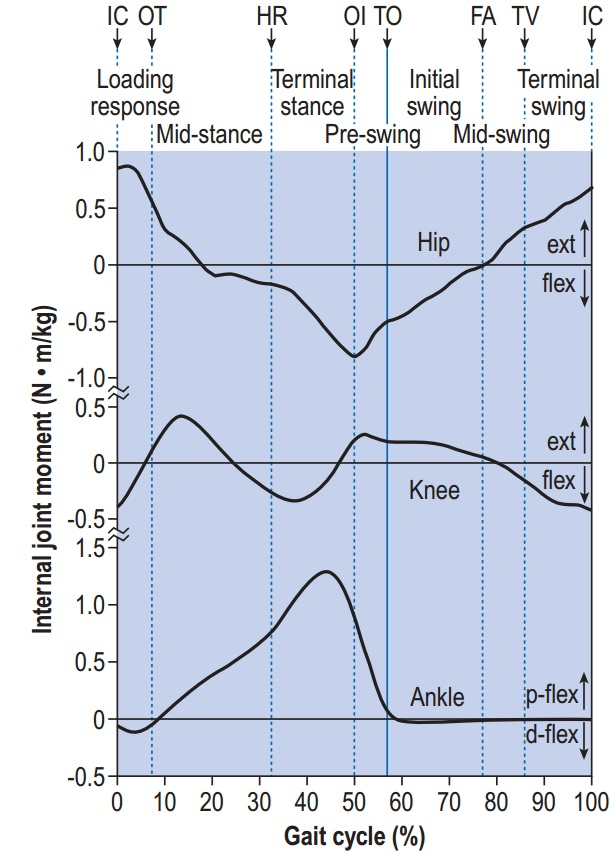
\includegraphics[width=8cm]{fig/f52.jpg}
    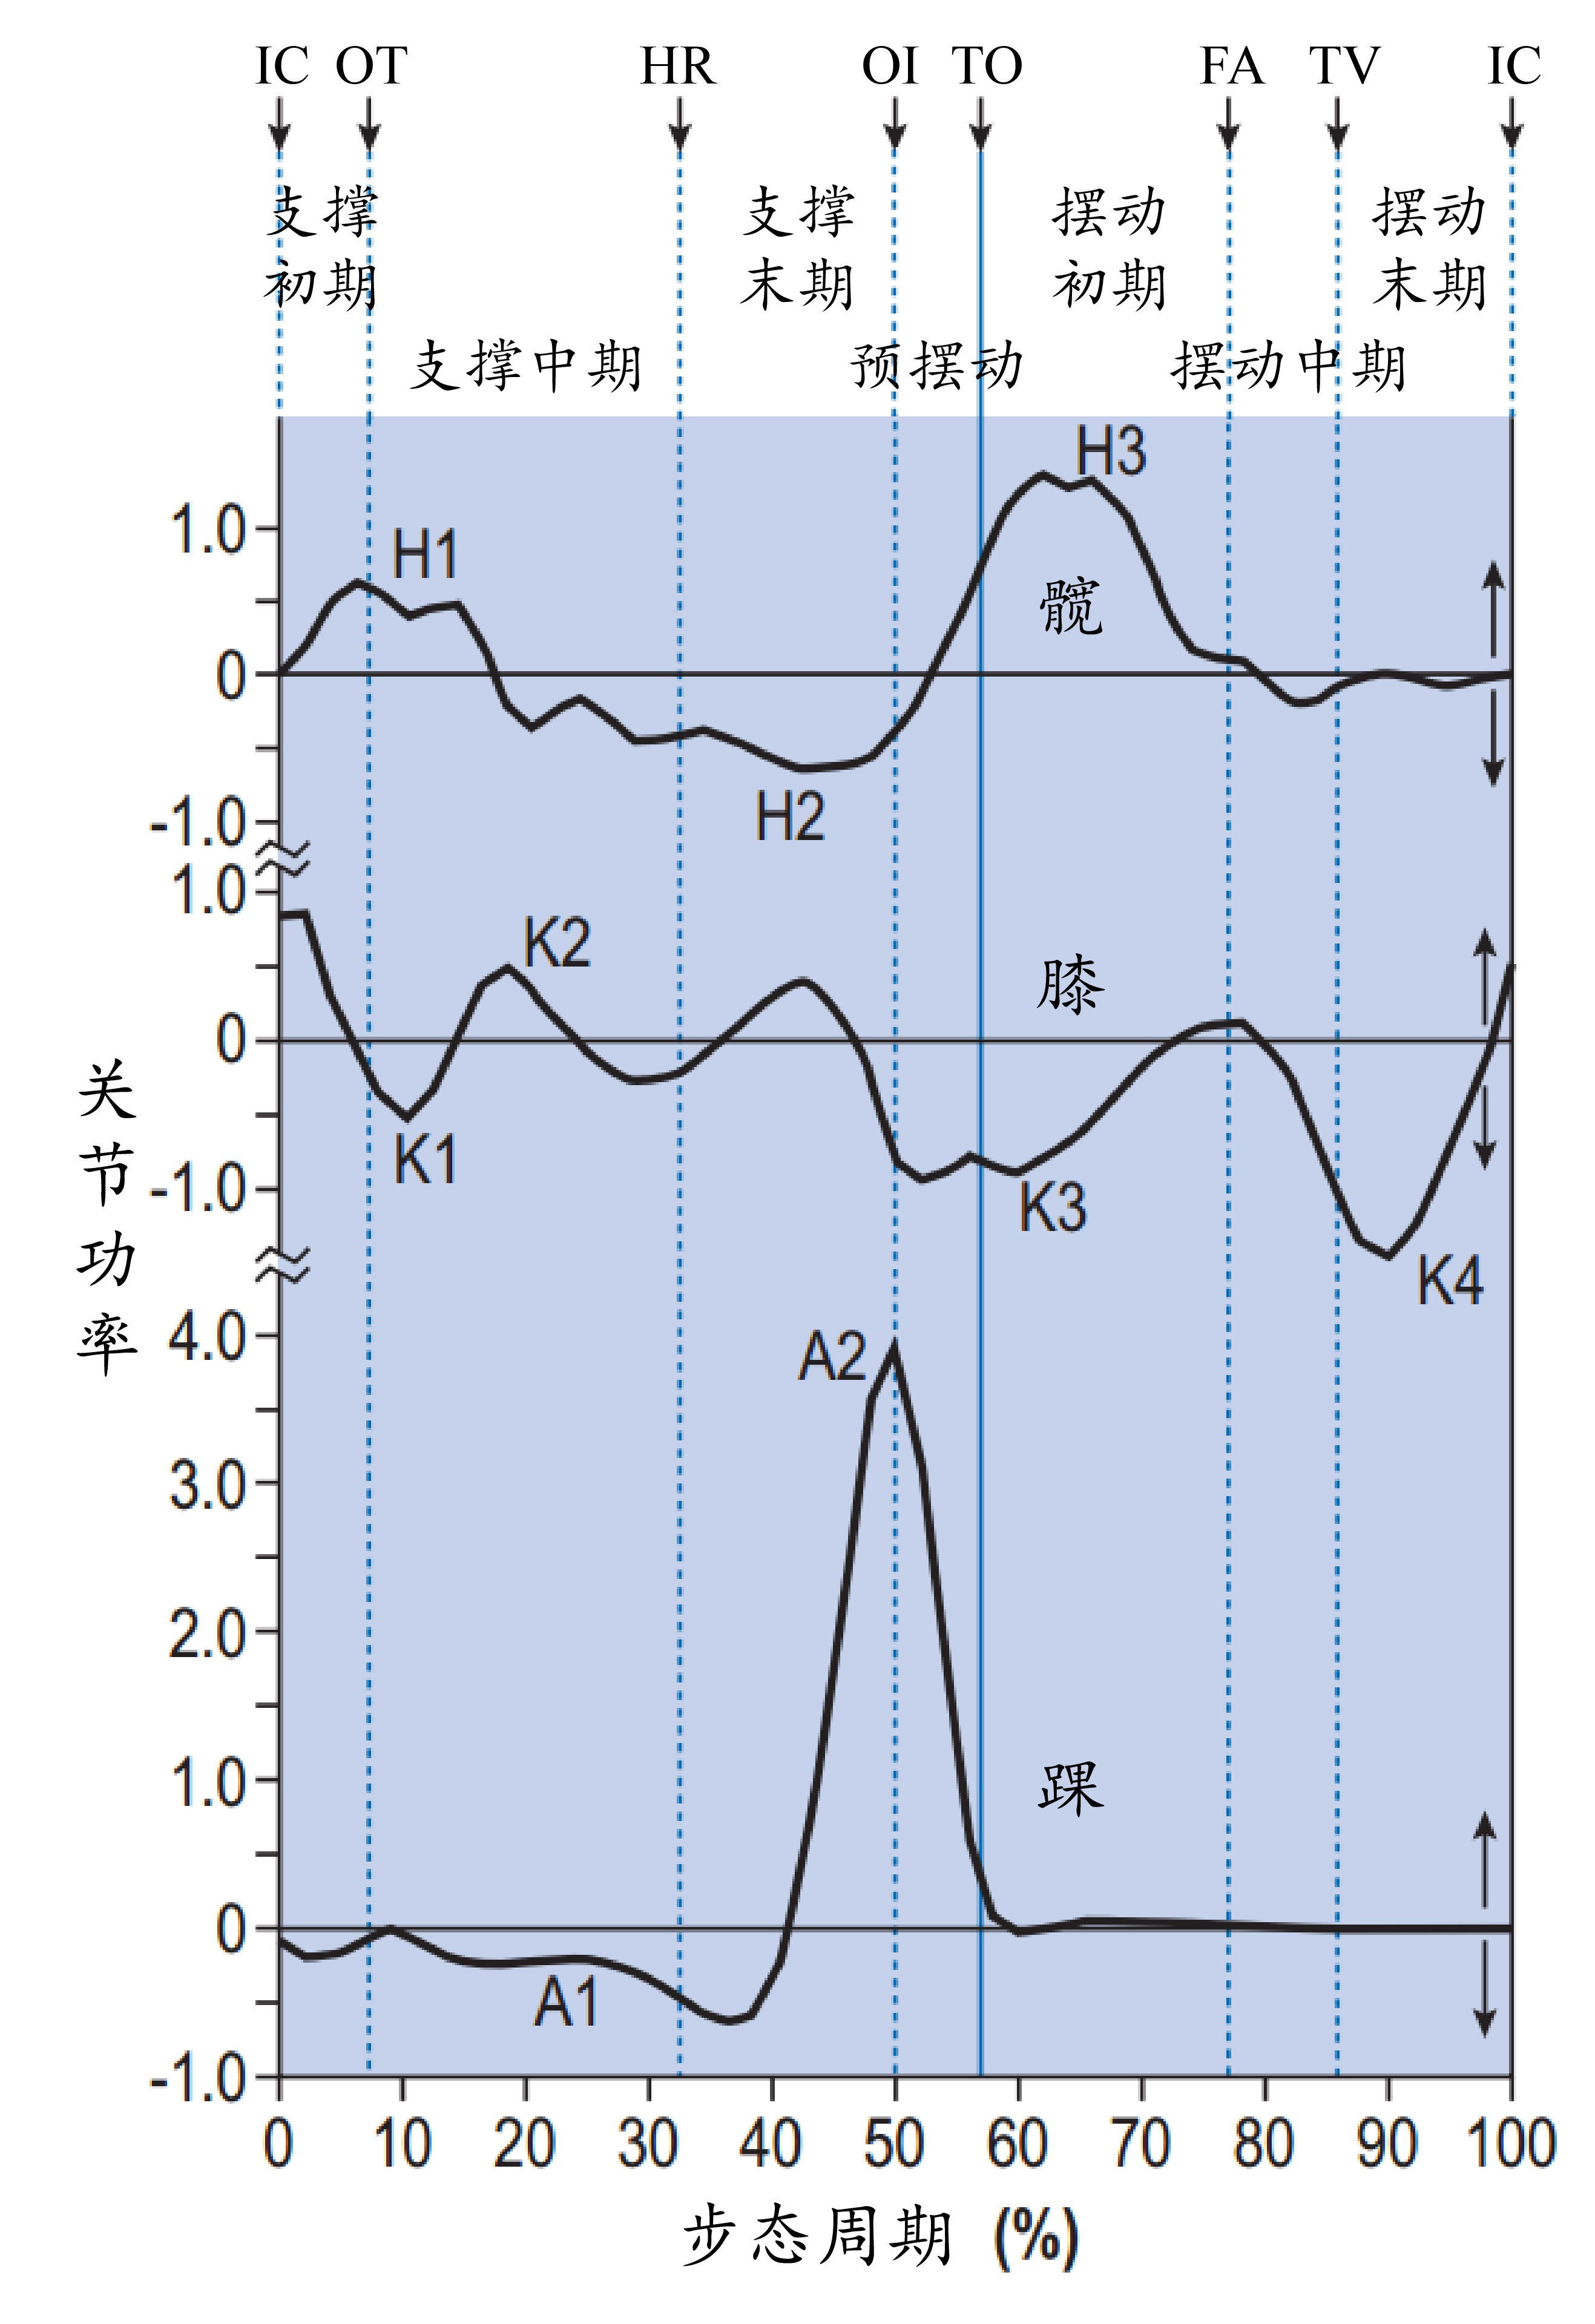
\includegraphics[width=8cm]{fig/f53.jpg}
    \caption{人体行走过程的关节力矩与关节功率\cite{p44}}
    \label{fig:subfigss}
\end{figure}

对于直接力矩控制的理解,可以从人体行走时自身的踝关节力矩出发。如图3.3所示,在步态周期的支撑阶段,踝关节持续施加一个作用力矩,且随着步态周期时间成单调上升和单调下降的过程,并且在即将地面时产生一个较大的关节功率输出。基于时间的直接力矩控制可以看做是一种稳态条件下的助力模式,通过外骨骼的辅助力矩减小人体自身的由肌肉产生的关节力矩,从而提供助力效果。

\begin{figure}[htb]
    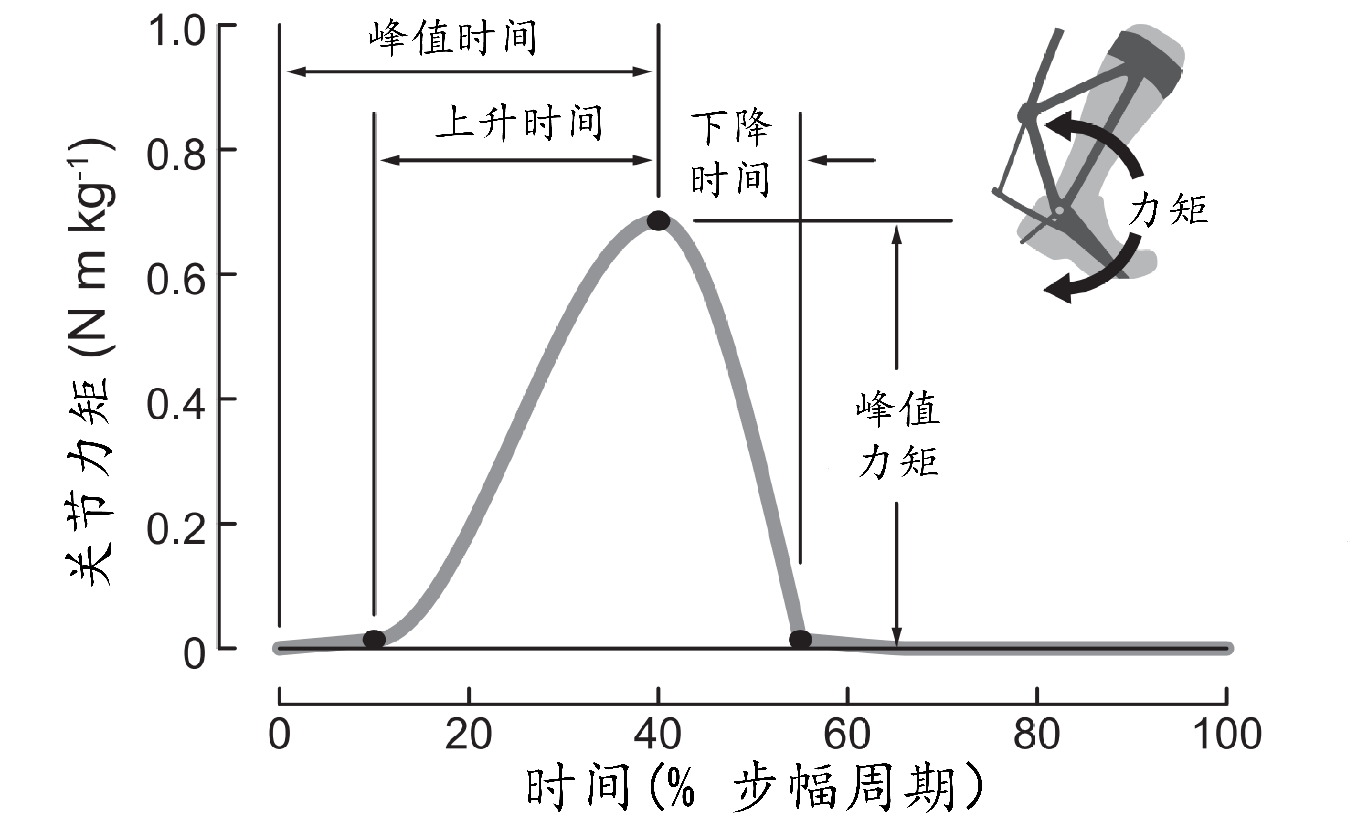
\includegraphics[width=15cm]{fig/f51.jpg}
    \caption{期望关节力矩曲线}
    \label{fig:mark}
\end{figure}

本文所使用的力矩曲线如图3.4所示。曲线由四个参数确定,分别为:
\begin{enumerate}
    \item 峰值力矩
    \item 峰值时间
    \item 上升时间
    \item 下降时间
\end{enumerate}
其中峰值力矩的单位为$N\cdot m \cdot kg^{-1}$,三个时间参数的单位均为步态周期的百分比。之后使用三次样条函数对力矩曲线进行插值,从而得到期望力矩的曲线。

由于直接力矩控制反应的是一种稳态条件下的助力模式,一组力矩曲线参数都表示一种独特的助力模式,且适合每个人的助力模式都不尽相同,因此需要针对每个穿戴者配置适合其行走的助力模式。对于本实验的受试者(本文作者),一组适合的助力参数如表3.1所示,后面所有的底层控制实验均在此参数下完成。

\begin{table}[htb]
    \caption[力矩曲线]{力矩曲线参数}
    \begin{tabular}{llll}
      \toprule
        峰值力矩 & 峰值时间 & 上升时间 & 下降时间 \\
      \midrule
        30 & 45 & 25 & 20 \\
      \bottomrule
    \end{tabular}
\end{table}

\section{底层控制算法}
                                                                                        
\subsection{PD反馈控制}
PID控制是控制理论中最简单最常见的控制方法,由于其简单、容易理解、方便调参的特点,广泛的在工业系统中。PID控制是反馈控制的一种基本形式,其中P为比例,D为微分,I为微积分。在实际应用中,根据实际需求的不同,PID控制器会有多种组合和变形。

\begin{align}
    u(t) = K_p \cdot e(t) + K_d \cdot \dot{e}(t) + K_i\int e(t) dt
\end{align}

PID控制器的三个部分各自具有不同的功能。比例项用来减小误差,代表着反馈控制本质,比例调节的参数$K_p$越大,则误差越小,响应速度越快。但参数过大时控制器会变得不稳定,在阶跃响应时会出现明显的超调现象。微分项的主要作用是减小由比例参数过大导致的超调问题,从二阶模型的角度来看,微分项的加入改变了系统的阻尼,因此微分调节也被称为阻尼调节。在真实的系统中,任何采集的信号都会含有噪声,噪声经微分后会被放大,因此微分项受噪声的干扰较为严重。积分环节主要是来消除稳态误差,在精度要求较高的场合下使用,但会减小系统的稳定性。由于本文所研究的底层控制器的输入信号为时变信号,属于随动跟踪系统,积分环节并不适合,所以最终使用PD控制器进行力矩控制。

\begin{figure}[htb]
    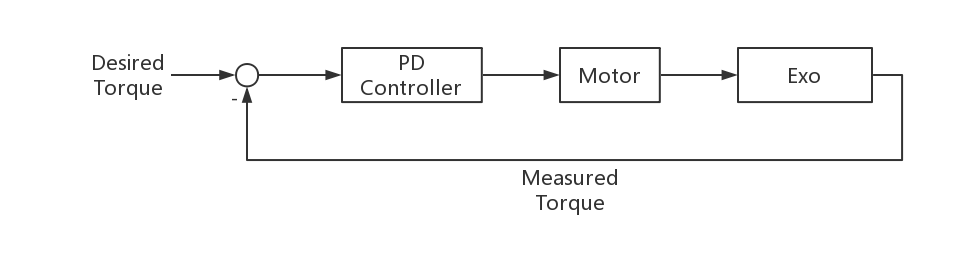
\includegraphics[width=15cm]{fig/f54.jpg}
    \caption{PD反馈控制的系统框图}
    \label{fig:mark}
\end{figure}

控制系统框图如3.5所示,PD控制器根据力矩误差产生电机的控制电压:
\begin{align}
    u(t) = K_p \cdot e(t) + K_d \cdot \dot{e}(t) \\
    e(t) = \tau_{des} - \tau_{real} \\
    \dot e(t) = \dot\tau_{des} - \dot \tau_{real}
\end{align}

\subsection{前馈控制}

将式(3.12)中的$\tau$换为期望力矩$\tau_{des}$可得:
\begin{align}
    \tau_{des} = K_t(\theta_p - \theta_eR)
\end{align}

对上式求导可得:
\begin{align}
    \dot\tau_{des} = K_t(\dot\theta_p - \dot\theta_e R)
\end{align}

整理得:
\begin{align}
    \dot\theta_p = \frac{1}{K_t}\tau_{des} + \dot\theta_e R
\end{align}

进一步忽略$\dot\theta_e R$,并考虑到电机减速比:
\begin{align}
    \dot\theta_m = \frac{N}{K_t}\dot\tau_{des}
\end{align}

带入式(3.5)得:
\begin{align}
    U_a &= \left(\frac{R_{a} f_{e}}{K_{a}}+K_{b}\right) \frac{N}{K_t} \dot\tau_{des} \\
        &= K_o \dot\tau_{des}
\end{align}

因为过程中的许多参数未知,所以参数$K_o$可以通过系统辨识或试错得到。

由于模型的不确定性和建模过程中简化,以单纯的前馈控制无法达到较好的控制效果,一般会与反馈控制相结合构成复合控制。具有前馈控制与PD反馈控制的系统框图如3.6所示。
\begin{figure}[htb]
    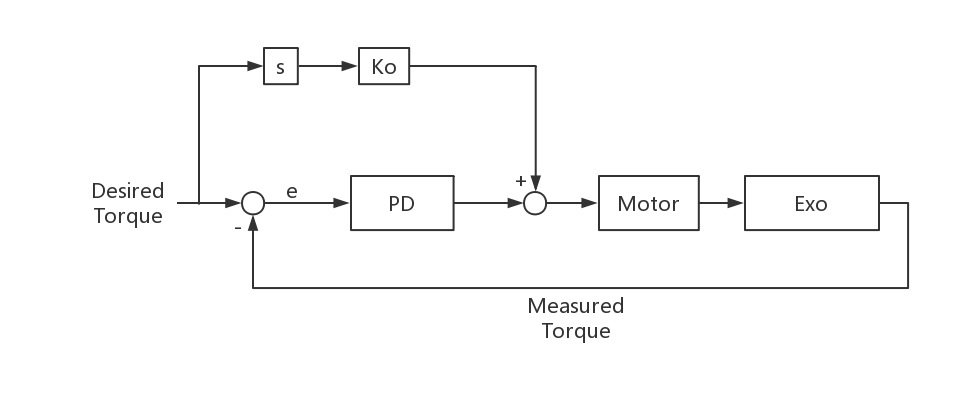
\includegraphics[width=15cm]{fig/f55.jpg}
    \caption{前馈+PD控制的系统框图}
    \label{fig:mark}
\end{figure}

\subsection{迭代学习控制}

迭代学习控制(Iterative Learning Control, ILC)属于智能控制的一种,最早由Uchiyama\cite{p46}于1978年首先提出。该控制方法适合具有重复运动性质的被控对象,它不依赖于系统精确的数据模型,能够以非常简单的方式处理不确定、非线性、强耦合的动态系统,且具有较高的跟踪精度。它通过反复应用先前试验得到的信息,以迭代的形式补偿系统复杂的动力学过程,产生优化输入信号,使系统输出尽可能逼近理想值。虽然步态过程不像工业机器人有固定的循环周期,但在稳定行走时也有着一种周期特性,因此可以使用迭代学习进行力矩控制。

本文采用Arimoto\cite{p47}提出的$D$型迭代学习控制律,假设外骨骼系统在第$n$个步态循环的第$i$个时刻力矩跟踪的误差为$e(i,n)$:
\begin{align}
    e(i,n) = \tau_{res} - \tau_{real}
\end{align}

迭代学习控制器根据$e(i,n)$通过周期迭代的方式学习一个输出序列$u(i,n)$,每个运动周期结束时更新一次迭代:
\begin{align}
    u(i,n+1) = u(i,n) + K_l\dot{e}(i+D,n)
\end{align}

其中参数$D$考虑了延时问题,$K_l$为迭代学习的误差学习参数。

迭代学习控制可以作为一个独立的控制器,也可以与其他控制器组合使用。单纯的ILC无法对抗扰动甚至胡不稳定,因此较多的将ILC与PD控制相结合,PD控制进行扰动抑制,ILC用于消除反馈控制所残留的轨迹跟踪误差,从而使跟踪达到更高的精度。

\section{力矩控制实验与分析}

本文对上一小节所提出的三种控制算法,设计了如下四种控制器形式,并进行了实验和对比:
\begin{enumerate}
    \item PD控制
    \item PD控制+前馈控制
    \item ILC
    \item PD控制+前馈控制+ ILC
\end{enumerate}

三种控制算法都需要进行参数整定以达到较好的控制效果。对PD控制器的参数本文使用曲线响应法进行整定,对于前馈控制和ILC的参数使用试错法。三种控制算法的最终参数如表3.2所示。

\begin{table}[htb]
    \caption[控制参数]{三种控制算法的参数值}
    \begin{tabular}{lllll}
      \toprule
        $K_p$ & $K_d$ & $K_o$ & $K_l$ & $D$ \\
      \midrule
        5 & 0.4 & 1 & 2 & 9 \\
      \bottomrule
    \end{tabular}
\end{table}

力矩控制实验时,受试者穿戴外骨骼以4.5$m/s$的速度在跑步机上稳定的行走。其中无ILC的控制器在参数调整一分钟后开始记录数据,含有ILC的控制器在学习稳定后开始记录。每个控制器记录两分钟,约120步的数据。

\begin{figure}[htb]
    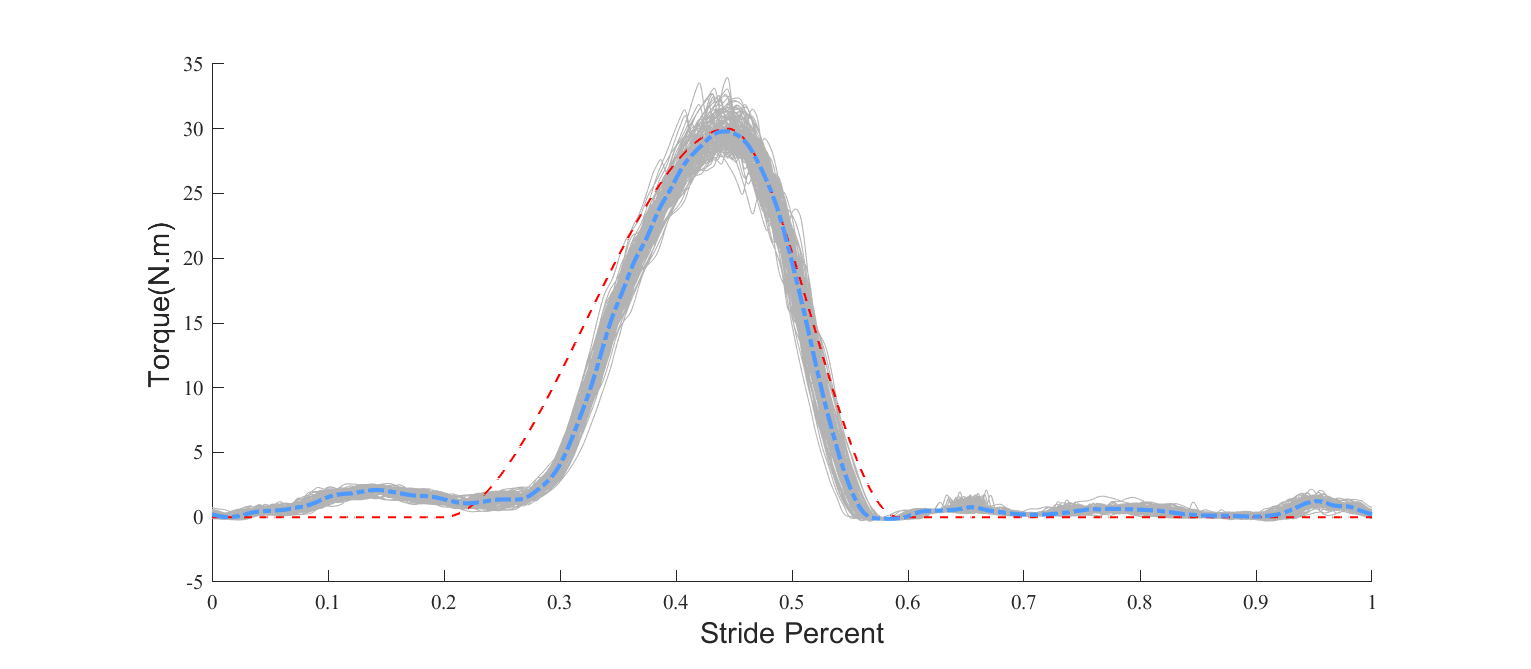
\includegraphics[width=17cm]{fig/f56.eps}
    \caption{PD控制的力矩跟踪效果}
    \label{fig:mark}
\end{figure}
\begin{figure}[!htb]
    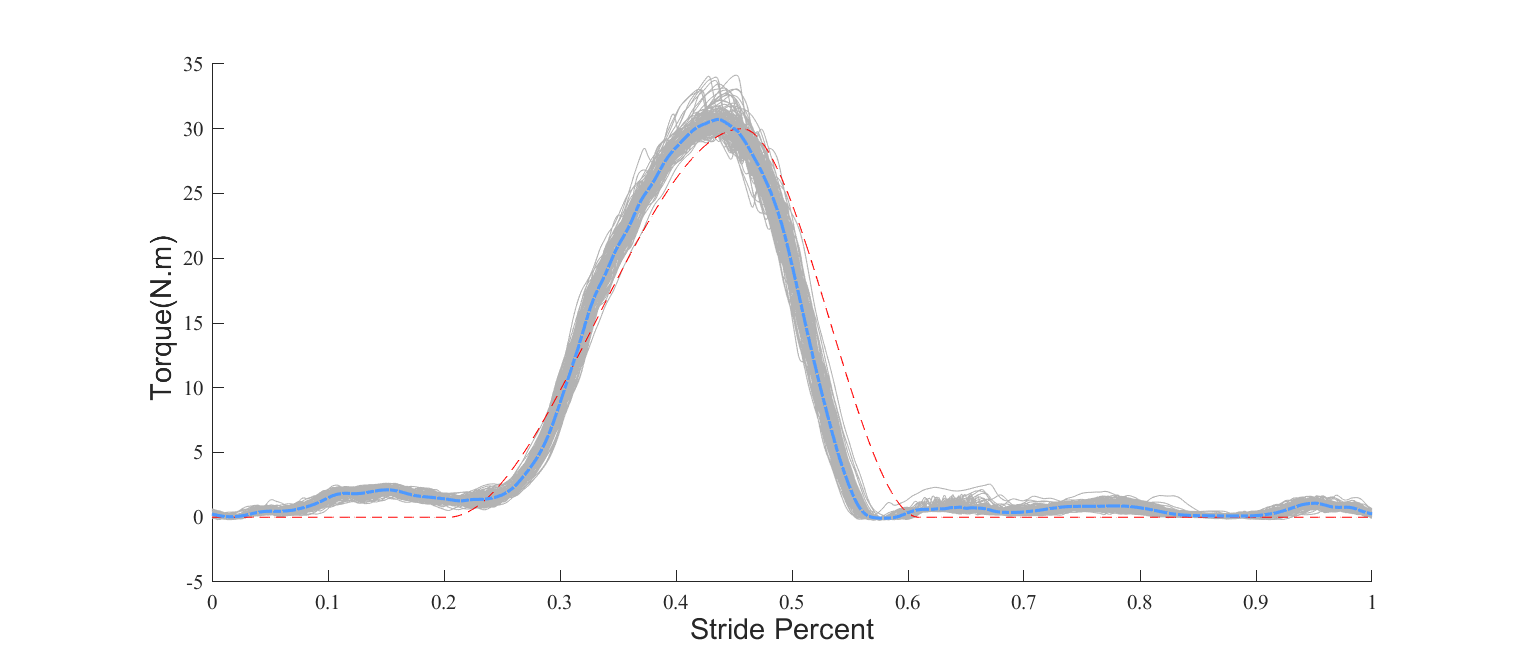
\includegraphics[width=15cm]{fig/f57.eps}
    \caption{PD+前馈控制的力矩跟踪效果}
    \label{fig:mark}
\end{figure}
\begin{figure}[!htb]
    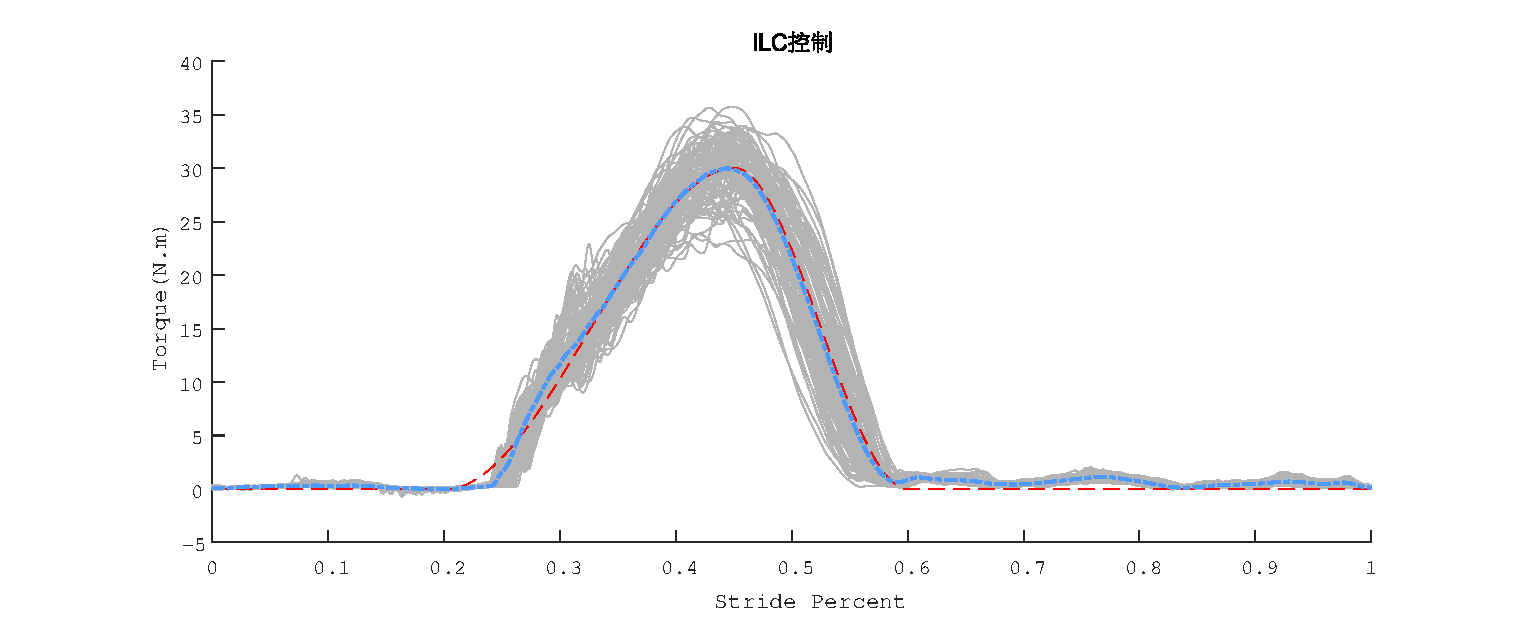
\includegraphics[width=15cm]{fig/f58.eps}
    \caption{ILC的力矩跟踪效果}
    \label{fig:mark}
\end{figure}
\begin{figure}[!htb]
    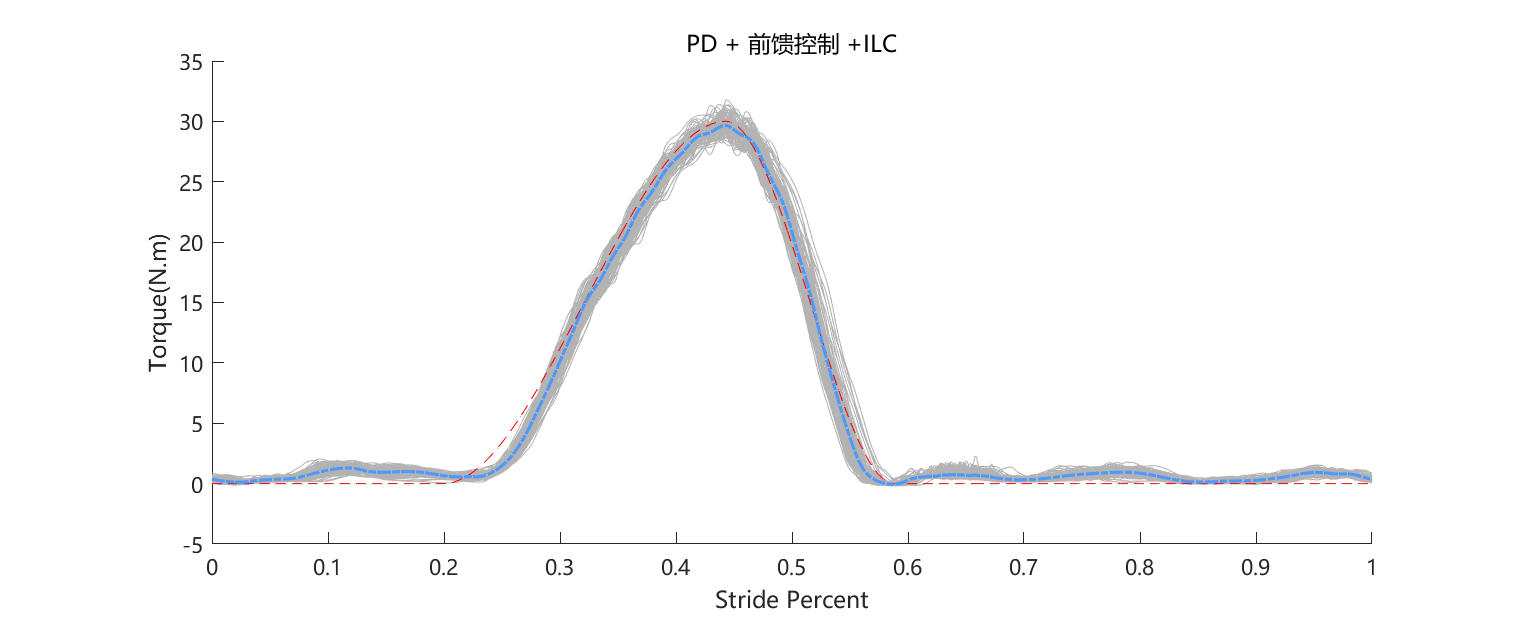
\includegraphics[width=15cm]{fig/f59.eps}
    \caption{PD+前馈+ ILC的力矩跟踪效果}
    \label{fig:mark}
\end{figure}

\begin{table}[htb]
    \caption[控制参数]{四种种控制器力矩追踪的均方根误差}
    \begin{tabular}{llll}
      \toprule
        PD & PD+前馈 & ILC & PD+前馈+ ILC \\
      \midrule
        2.226 & 1.729 & 1.605 & 0.968 \\
      \bottomrule
    \end{tabular}
\end{table}

实验结果如图3.7-3.10所示,图中红色虚线为期望力矩曲线,灰色实线为每一步实际的跟踪结果,蓝色实线为平均力矩跟踪结果,表3.3为四种控制器力矩跟踪的均方根误差。

由图3.8可以看出,加入前馈控制后力矩曲线上升阶段追踪效果较PD控制好,但在下阶段有较大误差,这可能是源于鲍登线拉和松两种状态的非线性。迭代学习控制平均的追踪效果较好,但对于扰动较为敏感,因此每一步的力矩跟踪波动较大。PD、前馈、ILC组合在一起时有相对较好的控制效果,追踪精度较高且波动范围较小。

\subsection{本章小结}

本章介绍了外骨骼力矩控制的上层控制器与底层控制器,上层控制器用来产生期望力矩曲线,底层控制器实现对期望力矩曲线的跟踪。针对所提出三种控制算法,设计了四种不同组合形式的控制器,并对其进行了验证与对比。实验结果表明,综合三种算法的控制器具有较好的力矩追踪效果。
\chapter{“人在环中”的外骨骼优化}

数十年来,科研人员提出了各式各样的控制算法,但无一例外地需要根据穿戴者去精心的调节各种参数,这些参数的调整多以经验和试错为主,并没有严格的标准。以BLEEX下肢外骨骼系统为例,BLEEX所使用的灵敏度放大算法非常依赖精确的动力学模型,针对不同的穿戴者需要设计不同的灵敏度放大系数,并通过不断试错的方式来得到最合适的参数。

由于人类个体之间生理学与神经学的差异,每个人都有其偏好的行走习惯和行走模式,对外骨骼不同助力模式的感受不尽相同,不同个体对同一助力模式的反应也大相径庭。只有为穿戴者提供最适合的助力模式,才能真正的实现有效辅助与人体机能提升。因此,寻找适合穿戴者的助力模式是一项非常有挑战性的工作。

\begin{figure}[!htb]
    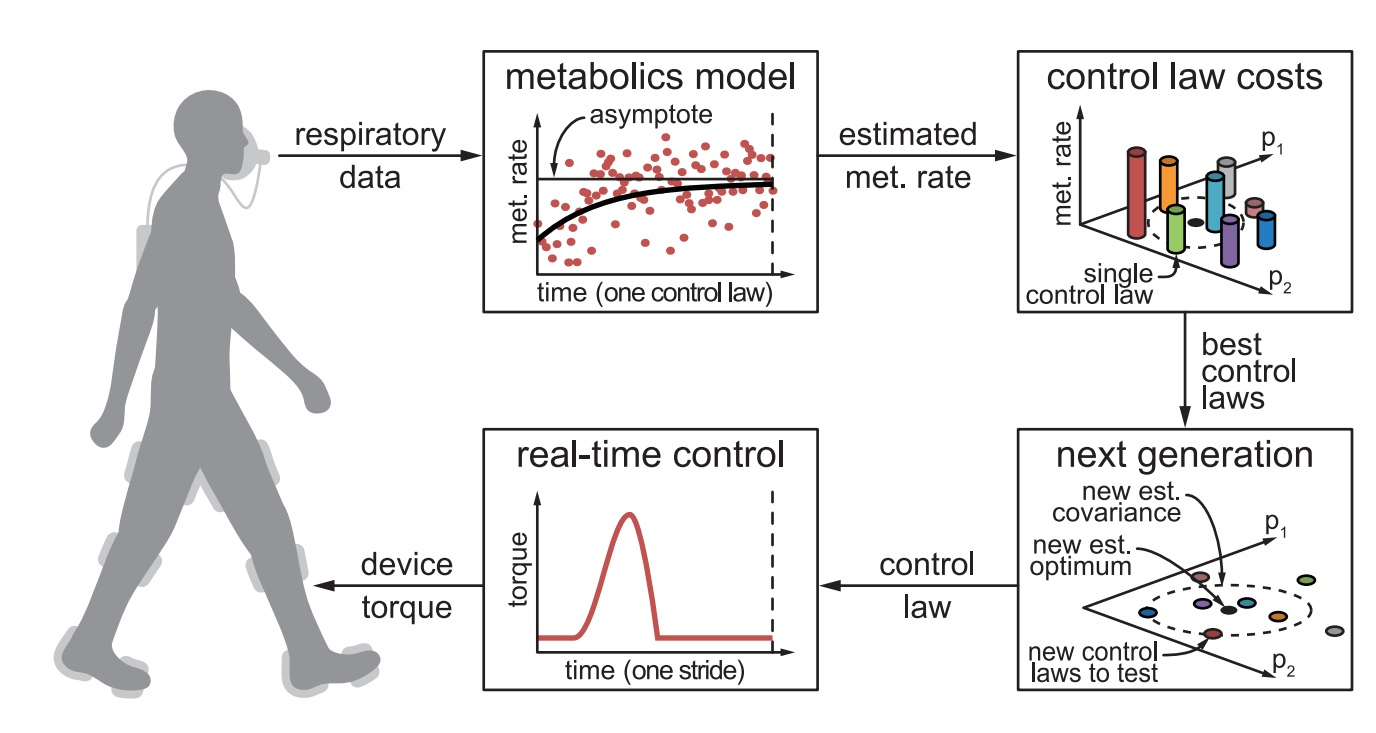
\includegraphics[width=15cm]{fig/f60.jpg}
    \caption{“人在环中”的优化方法\cite{p40}}
    \label{fig:mark}
\end{figure}

“人在环中”的优化方法正是在这种背景下被提出。针对不同的个体,根据其对助力模式反应,在助力行走过程中实时的调整助力参数,以达到为穿戴者提供最佳的助力模式,这种方法被称为“人在环中”的优化方法。在这种方法中,穿戴者成为外骨骼系统环路的一部分,为助力参数的选择提供反馈信息,如图4.1所示。
\begin{align}
    p^{*} & = \mathop{min}\limits_{p} f(p) \\
    f(p):\quad &p \to adaptedness
\end{align}

“人在环中”的优化方法把调整助力参数的过程看做是一个优化问题,其中适应度为助力参数的函数,通过优化适应度函数的最小值来得到穿戴者最适合的助力参数。然而适应度函数并不是一个具有显示表达的目标函数,也不是一个可以描述的确定过程,而是穿戴者在与外骨骼交互的过程中产生的一个生理信号。由于人体生理及运动过程太过复杂,无法进行建模,所以适应度函数是未知的,只能通过实时的采样得到。因此“人在环中”的优化本质上是一个黑箱优化,而且是一个目标函数采样困难、含有噪声的黑箱优化问题。

任何一个足够复杂的系统都可以视为黑箱模型。研究人员探索了许多用于黑箱优化的算法\cite{p48},如随机搜索、遗传算法、模拟退火、单纯形法、贝叶斯优化等等。但由于进行“人在环中”优化时,人体的生理反馈信号含有巨大的噪声,因此很多方法并不适用。在现有的研究成果中,协方差矩阵自适应进化策略\cite{p40}(CMA-ES)和贝叶斯优化\cite{p41}(BO),已被证明是两种可行的方案。

本章针对“人在环中”的优化问题,使用人体肌肉活跃度为生理反馈,通过贝叶斯优化的方法对上层控制的两个控制参数进行优化,在20次迭代内完成最优参数的辨识。

\section{贝叶斯优化}

贝叶斯优化的核心为贝叶斯定理:
\begin{align}
    p(f|D_{1:t})=\frac{D_{1:t}|p(f)}{p(D_{1:t})}
\end{align}

其中$f$表示位置的目标函数,$D_{1:t} = \{(x_1,y_1),\cdots,(x_t,y_t)\}$表示既有数据集;$p(D_{1:t}|f)$为数据集中观测量的似然分布,反应了观测数据的噪声;$p(f)$表示$f$的先验概率分布,即对前一步对目标函数的估计;$p(f|D_{1:t}$表示$f$的后验分布,即在观测后对目标函数的更新估计。

贝叶斯优化是一种序贯优化方法,它在每一次对目标函数采样后,主动选择下一个合理的参数进行采样,从而尽快的达到最优解。本质上来说,贝叶斯优化通过利用历史信息,用代理模型拟合真实目标,根据对拟合模型的估计,产生一个“最有意义”的采样点,不断迭代从而实现快速而高效的优化。

贝叶斯优化主要由两部分组成:用于拟合观测数据的概率代理模型和产生新采样点的采集函数。本文所使用的概率代理模型和采集函数分别为高斯过程模型和LCB采集函数。

高斯过程(GP)是一种常用的非参数模型,用以对未知目标函数进行拟合,广泛应用在回归、分类等领域。高斯过程由一个均值函数和一个协方差函数构成:
\begin{align}
    f(x)\sim \mathcal{GP}(m(x),k(x,x'))
\end{align}

由Sherman-Morrison-Woodbury公式\cite{p49}可得,在数据集为$D_{1:t} = \{(x_1,y_1),\cdots,(x_t,y_t)\}$时,高斯过程可表示为:
\begin{align}
    P(f|D_{1:t},x) &= N(\mu_t(x),\sigma^2(x)) \\
    \mu_t(x) &= \mathbf{k}^T\mathbf{K}^{-1}\mathbf{f}_{1:t} \\
    \sigma^2(x) &= k(\mathbf{x},\mathbf{x}) - \mathbf{k}^T\mathbf{K}^{-1}\mathbf{k}
\end{align}

其中
\begin{align}
\mathbf{K} & =\left[ \begin{array}{ccc}{k\left(\mathbf{x}_{1}, \mathbf{x}_{1}\right)} & {\dots} & {k\left(\mathbf{x}_{1}, \mathbf{x}_{t}\right)} \\ {\vdots} & {\ddots} & {\vdots} \\ {k\left(\mathbf{x}_{t}, \mathbf{x}_{1}\right)} & {\dots} & {k\left(\mathbf{x}_{t}, \mathbf{x}_{t}\right)}\end{array}\right] \\
\mathbf{k}&=\left[k\left(\mathbf{x}, \mathbf{x}_{1}\right) \quad k\left(\mathbf{x}, \mathbf{x}_{2}\right) \quad \cdots \quad k\left(\mathbf{x}, \mathbf{x}_{t}\right)\right] \\
k &\left(\mathbf{x}_{i}, \mathbf{x}_{j}\right)=\exp \left(-\frac{1}{2}\left\|\mathbf{x}_{i}-\mathbf{x}_{j}\right\|^{2}\right)
\end{align}

采集函数用来选择下一次优化迭代的采样点。在进行采样点选取时,有两个基本的出发点:
\begin{enumerate}
    \item 对均值函数最小值处进行采样,提高对最优参数估计精度
    \item 对方差函数最大值处进行采样,以降低模型估计的不确定度
\end{enumerate}

前者表示对模型的利用,后者表示对模型位置的探索。任何一种采样函数都需要在探索和利用之间进行权衡,使得优化算法能够得到较高精度的全局最优解。其中LCB方法就是其中一种典型的采集函数:
\begin{align}
    LCB(x) = \mu(x) - k\sigma(x)
\end{align}

超参数$k$用来调节探索与利用之间的比重,$k$越大则越倾向于对未知进行探索。通过求取函数$LCB(x)$的最小值,即可得到下一次优化迭代需要采样的参数。

\begin{algorithm}[h]
    \caption{贝叶斯优化}
    \begin{algorithmic}[1]
    \FOR{$i = 1,2,\cdots$}
    \STATE 最小化高斯过程的采集函数,得到采样参数:$x_t=\mathop{min}\limits_{x}LCB(x)$\
    \STATE 对目标函数进行采样:$y_t = f(x_t)+\epsilon_t$\
    \STATE 更新高斯过程:$D_{1:t} = \{ D_{1:t-1},(x_t,y_t)\}$
    \ENDFOR
    \end{algorithmic}
\end{algorithm}

贝叶斯优化的算法流程如上所示,每一次迭代开始时当前对目标函数估计的高斯过程,计算采集函数的最小值,得到本次迭代的参数,之后对目标函数进行采样,最后用观测到的数据更新高斯过程。贝叶斯优化可以看做是一个具有想象力的算法,它从已有数据想象出目标函数的大致形状,并选择有价值的点进行采样,以调整自己的想象,使得估计的参数不断地向最优参数靠近并收敛。

\section{基于肌肉激活指标的生理反馈信号}

为了实现“人在环中”优化,必须要选择合适的人体生理信号进行反馈,目前使用较多的反馈信号为人体的代谢耗能,但代谢耗能数据获取较为困难,需要两分钟才能完成一次目标函数的采样,时间成本较高。因此本文选择人体肌电信号作为生理反馈。
\begin{figure}[htb]
    \subfloat[步态过程关节力矩]{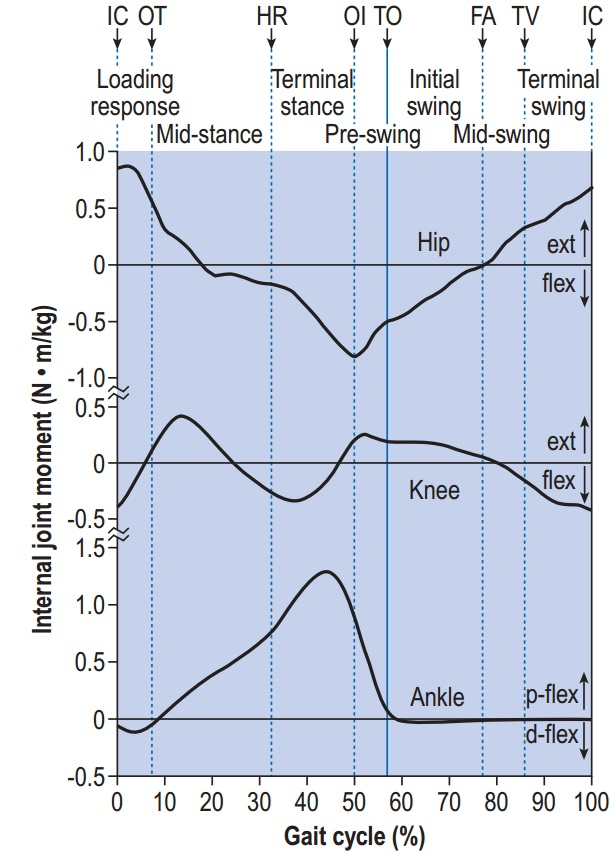
\includegraphics[width=8.9cm]{fig/f52.jpg}}
    \subfloat[步态过程腿部肌肉激活度]{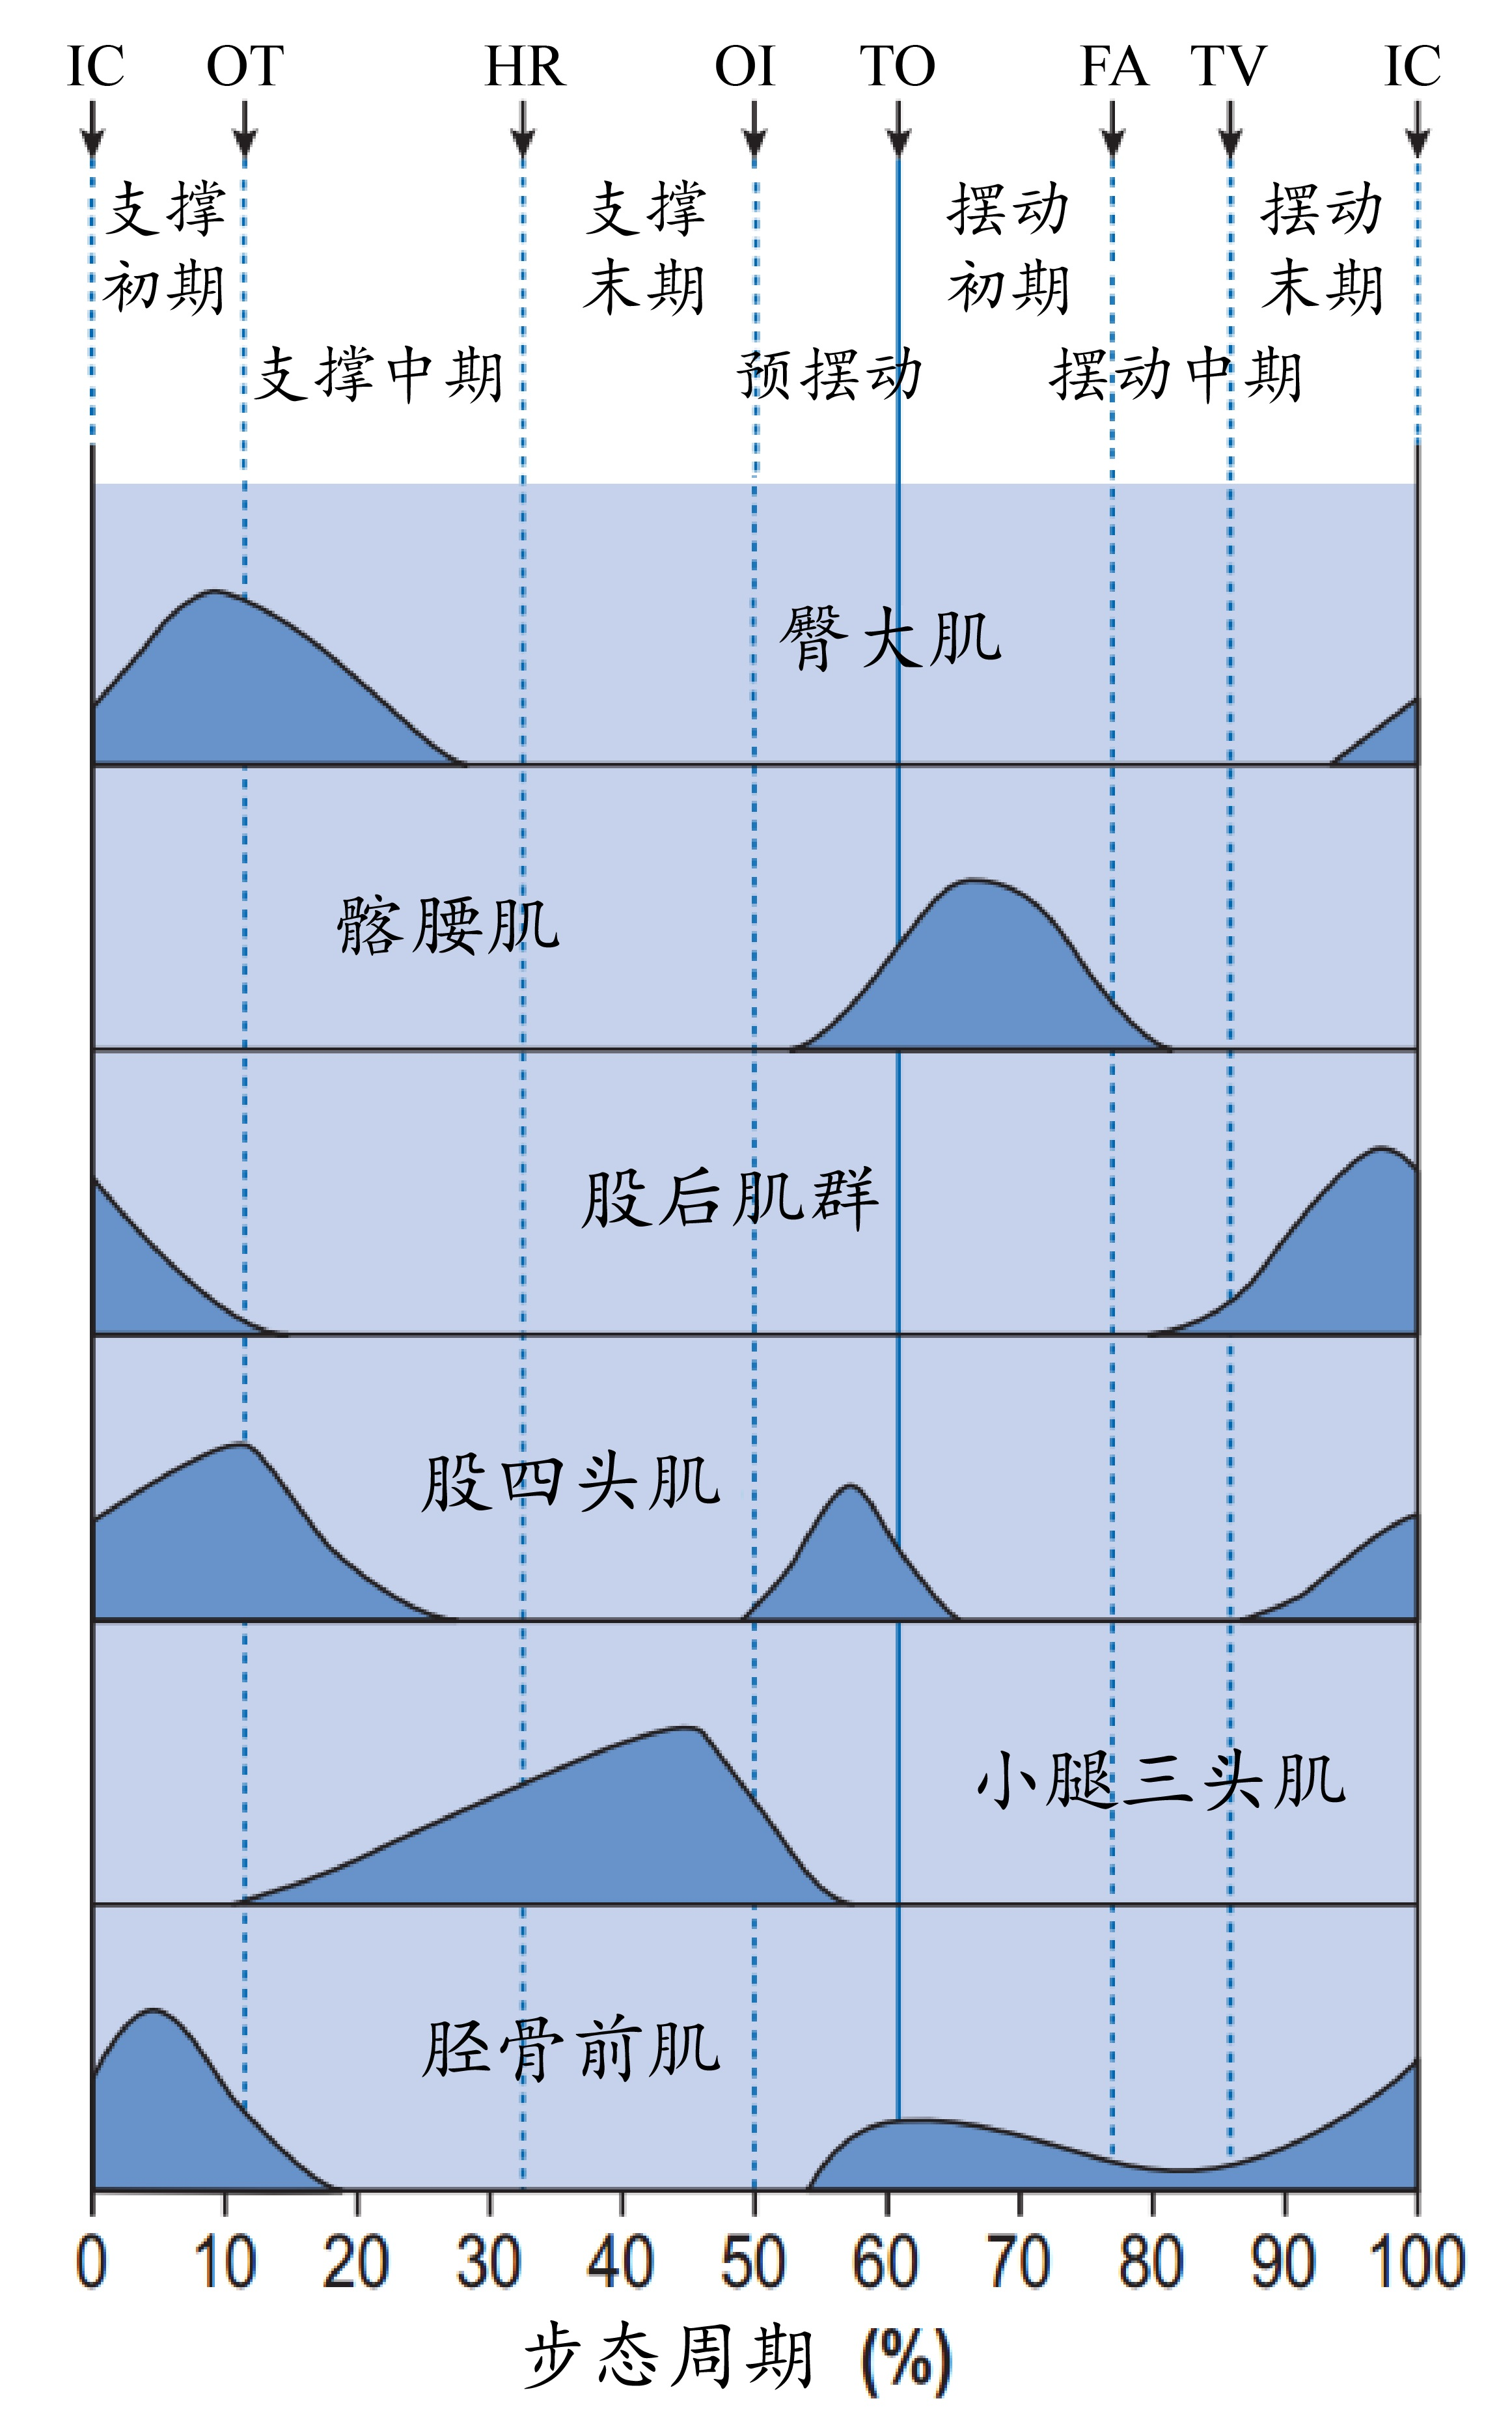
\includegraphics[width=8cm]{fig/f62.jpg}}
    \caption{步态过程的关节力矩与肌肉激活\cite{p44}}
    \label{fig:subfigss}
\end{figure}

行走时人体踝关节的运动主要受小腿三头肌和胫骨前肌控制,其中小腿三头肌由腓肠肌和比目鱼肌组成,控制髋关节拓屈,而胫骨前肌位于小腿前侧,控制髋关节背屈。比较图4.2中关节力矩曲线与肌肉激活度,可以看出小腿三头肌的收缩与踝关节力矩比较相似,而踝关节力矩与外骨骼助力紧密相关。因此可以考虑用肌肉的激活度来衡量穿戴者对助力模式的反应,若助力模式能够为人体提供有效辅助,则穿戴者的肌肉激活水平会随之而下降。

本文选择了腓肠肌内侧、比目鱼肌和胫骨前肌三块肌肉的每个周期激活度均方根之和作为肌肉激活指标进行生理信号反馈,其中肌肉的激活度由EMG信号经滤波后得到。为了确认所选择的生理反馈信号能够用于优化实验(在优化空间内具有明显的最小值),本文先对该生理反馈信号的有效性进行了验证,在优化参数空间内选择45个点进行采样,每个点的采样持续30s(约30个步态循环),之后对采集到的数据在参数空间内进行三维插值,得到目标函数关于优化参数的近似估计。如图4.3所示,肌肉激活指标以热力图的形式进行显示,图中蓝色区域表示肌肉激活水平较低,此区域的助力模式比较适合受试者。实验结果验证了肌肉激活指标作为生理反馈的有效性。
\begin{figure}[!htb]
    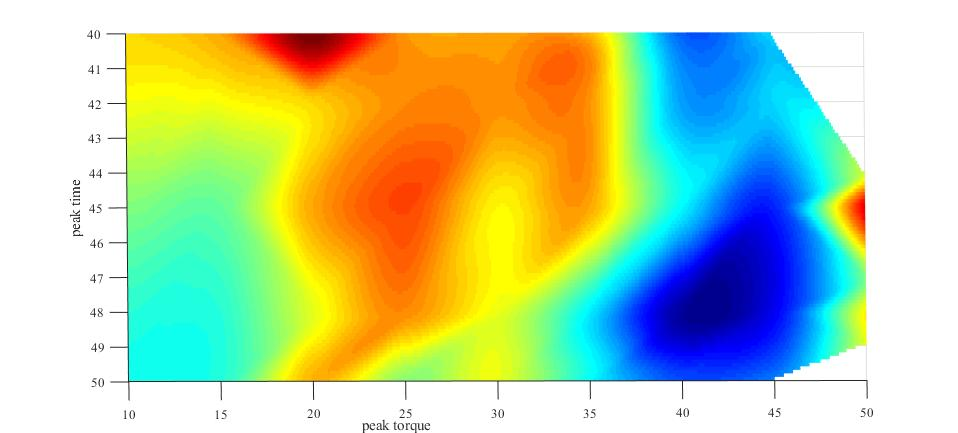
\includegraphics[width=17cm]{fig/f63.jpg}
    \caption{肌肉激活指标关于力矩参数近似估计}
    \label{fig:mark}
\end{figure}

\section{“人在环中”的外骨骼助力参数优化实验}

本文使用贝叶斯优化的方法,选择肌肉活跃度为生理反馈信号,对外骨骼力矩控制上层控制器的峰值力矩和峰值时间两个参数进行优化。

实验时受试者(本文作者)处于连续行走状态,每间隔15步进行一次优化迭代,每次迭代使用15步中最后5步肌肉活跃度的平均值作为生理反馈,更新最优估计并进行下一次迭代。优化迭代30次后认为优化收敛并停止优化,取30代的最优估计作为优化结果,即受试者的最优助力参数。优化完成后进行验证实验,分别记录受试者在外骨骼不施加辅助与施加最优助力参数下30步的肌肉激活水平。整个过程在相同实验条件下重复5次,每两次实验之间休息10分钟。
\begin{table}[htb]
    \caption[控制参数]{5次优化实验的最优助力参数}
    \begin{tabular}{llllll}
      \toprule
        峰值力矩 $N\cdot m$ & 43.8 & 46 & 43.6 & 47.6 & 44.6 \\
      \midrule
        峰值时间 $\%$ & 49.6 & 50 & 49.1 & 46.5 & 48.9 \\
      \bottomrule
    \end{tabular}
\end{table}

实验结果如表4.1和图4.4所示,峰值力矩分布在$45N\cdot m$左右,峰值时间分布在$49\% stride time$左右。优化结果与4.2小节的先验实验相一致,且符合受试者(本文作者)的主观感受。
\begin{figure}[htb]
    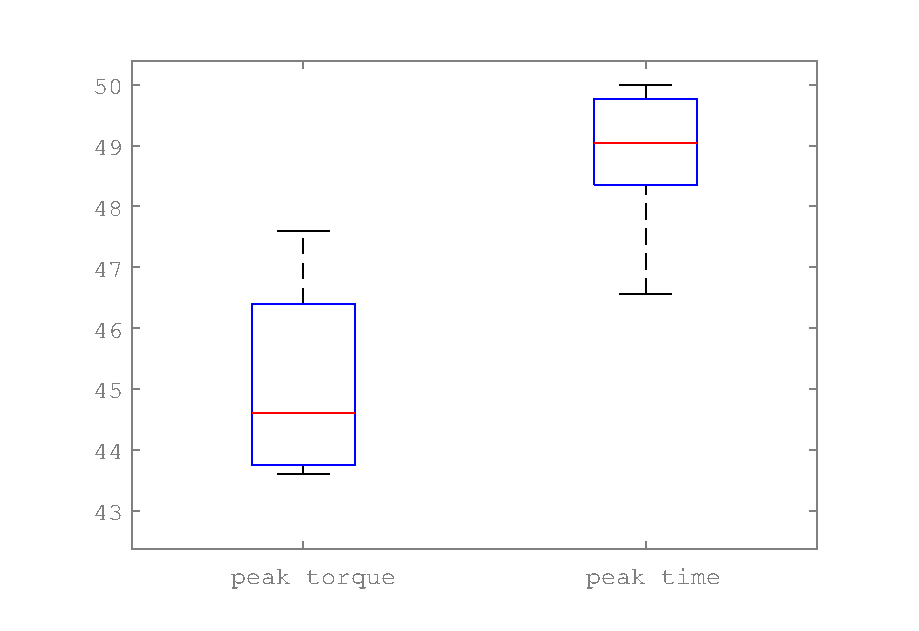
\includegraphics[width=11cm]{fig/f64.eps}
    \caption{最优助力参数的分布}
    \label{fig:mark}
\end{figure}
\begin{figure}[!htb]
    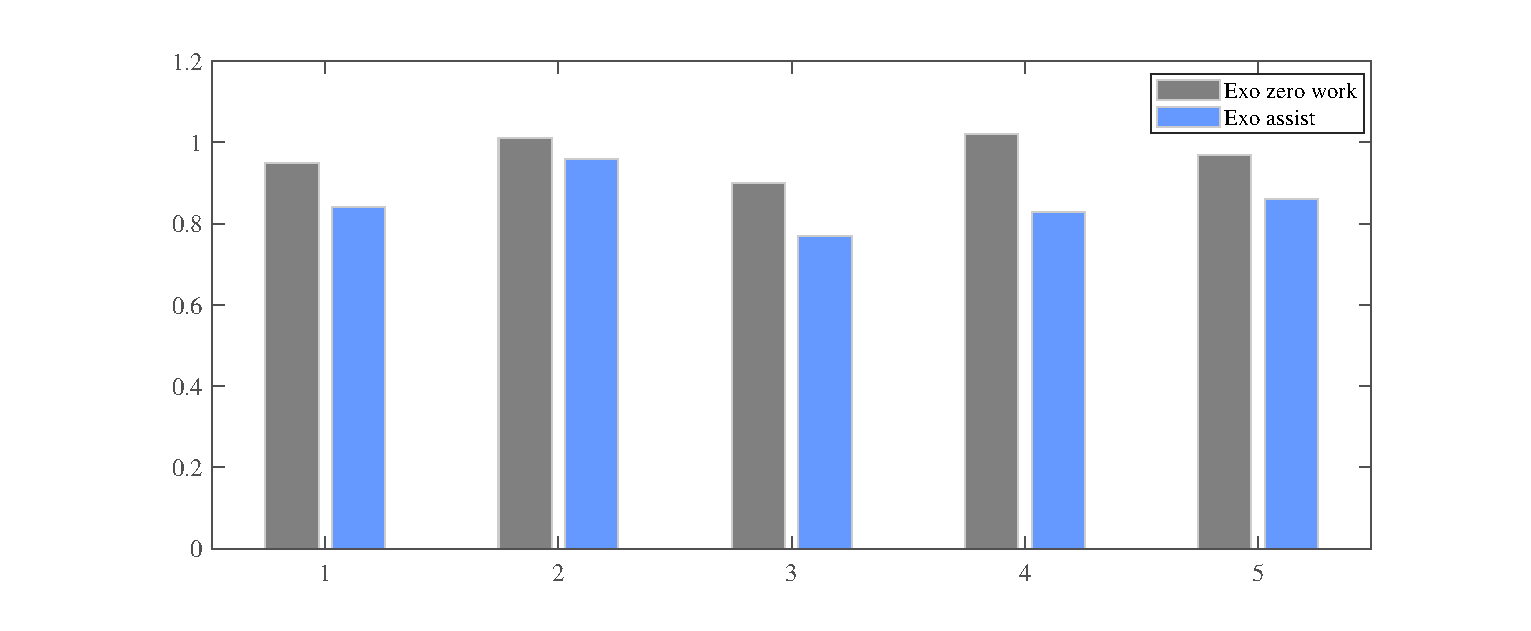
\includegraphics[width=17cm]{fig/f65.eps}
    \caption{最优助力参数的分布}
    \label{fig:mark}
\end{figure}
\begin{table}[!htb]
    \caption[控制参数]{优化参数下肌肉激活水平的下降程度}
    \begin{tabular}{cc}
      \toprule
      平均肌肉激活水平百分比 & 最大肌肉激活水平下降百分比 \\
      \midrule
        12.2\% & 18.6\% \\
      \bottomrule
    \end{tabular}
\end{table}

图4.5与表4.2显示了验证实验的结果。可以看出由优化得到的最优助力模式,均能够显著降低受试者的肌肉激活水平,其中平均肌肉激活水平下降12.2\%,最大下降18.6\%。

\section{本章小结}

本章针对外骨骼系统助力模式的调整问题,研究了“人在环中”的外骨骼参数优化方法。通过采集穿戴者对助力模式的生理反应,将其反馈至优化求解器中,不断迭代寻找最适合穿戴者的助力模式,从而充分发挥外骨骼潜能。实现上,本文采用贝叶斯优化方法,并选取基于EMG信号的肌肉激活指标作为生理反馈,通过实验验证了优化的有效性,并提高了时间效率。
\chapter{结论}
\section{研究内容总结}

本文主要对踝关节外骨骼的控制系统进行了研究,主要工作总结如下:

(1)搭建了外骨骼的传感系统。针对所研究的踝关节式外骨骼,搭建了基于应变片的外骨骼力矩测量模块、基于足底开关的步态周期检测模块、基于EMG信号和肌肉激活度检测模块、基于IMU的人体姿态数据采集系统。

(2)设计了外骨骼力矩控制系统。力矩控制由上层控制器与底层控制器组成,上层控制器用来产生期望力矩曲线,底层控制器实现对期望力矩曲线的跟踪。针对上层控制器,本文采用基于时间的直接力矩控制器,通过三次函数插值得到期望力矩曲线。针对底层控制器,本文提出了三种控制算法,设计了四种不同组合形式的控制器。

(3)研究了“人在环中”的外骨骼优化方法。针对外骨骼助力模式因人而异的问题,采集穿戴者的生理信号做目标函数,对助力参数进行优化,通过迭代寻找最适合穿戴者的助力模式,从而充分发挥外骨骼潜能。本文采用贝叶斯优化,并选取肌肉激活指标作生理反馈,通过实验验证了优化的有效性。

\section{课题展望}

本文对外骨骼系统中的传感、控制与优化问题进行了一系列基础工作,在此基础上对未来的研究工作有如下几点展望:

(1)搭建多传感器融合的外骨骼系统。控制系统非常依赖由传感系统得到的反馈信息,因此可靠、准确、稳定的传感数据对外骨骼系统而言至关重要。本文研究过程中多次出现由传感器数据不稳定而导致的系统故障,后续会从多传感器数据融合的角度出发,搭建更为可靠的传感系统。

(2)尝试多种上层力矩控制策略。本文研究的期望力矩曲线是基于时间的函数,只能作为稳态行走时的助力模式。后面将进一步研究在不同上层控制器下力矩控制的效果。

(3)“人在环中”优化最为一个较新的研究领域,至今还有很多问题函待解决。本文的优化研究最为一个尝试,初步证明了基于肌电的生理反馈可以用于优化。但更合适的生理反馈形式,更高效的优化算法,仍有待进一步探讨。

\appendix
% 如果需要附录的话,在这里 include
%\chapter{查重和其他注意事项}

本节由 Old Jack 写于 2017年六月\footnote{\url{https://github.com/nuaatug/nuaathesis/commit/1155207}}。

\section{查重}

先说结论:{\large\textbf{知网完全支持pdf查重}}。

这个问题是鄙人整个毕设过程中最担心的问题之一,从知乎以及其他各种渠道搜索的结果并不一致;另外关于pdf查重具体检测哪些部分也是有很多种说法,现在根据鄙人论文的检测结果来说明一下几个需要注意的地方:

\begin{itemize}
  \item \textbf{页眉页脚:} pdf的眉页脚在论文查重检测范围内。如果担心会提升重复率,可以将页眉文字去掉(个人认为没必要);
  \item \textbf{公式环境:} pdf中的公式在论文查重检测范围内。所以在编辑公式的时候,可以考虑不使用传统符号来编辑公式(物理公式符号不建议使用这种方法,各物理量的符号比较固定,老师可能会要求改正),以降低重复率,如参考文献中使用$\alpha$,可以改为$a$或$x$诸如此类;
  \item \textbf{表格环境:} 鄙人的论文中没有直接证据,但根据公式环境在查重检测范围内,鄙人推断表格的标题和内容很有可能也在范围内,所以建议大家不要直接摘抄实验数据和表格标题;
  \item \textbf{参考文献:} 鄙人在使用淘宝知网论文检测时,并未提交参考文献部分,学校不提供论文检测结果,所以目前没有直接证据证实参考文献是否在查重范围之内;
  \item \textbf{附录:} 鄙人的论文没有附录,情况不明。
\end{itemize}

鄙人的老师开始也要求上交word版论文,但是在鄙人的坚持下,最终上交了pdf版并成功通过查重。建议大家提前和指导老师打好招呼,最后提交pdf格式的论文。

\section{批注}
在论文撰写过程中,批注成了一个问题,鄙人的指导学姐并不是计算机专业出身,对\LaTeX 和基于Git的版本管理并不了解,所以沟通的途径就只有使用Adobe Acrobat等软件,对pdf文件本身进行批注,相比于word确实有些麻烦。

个人还是推荐使用Git\footnote{\url{https://git-scm.com/}}、Beyond Compare\footnote{\url{https://www.scootersoftware.com/}}等工具,辅以\LaTeX 本身的注释进行批注以及版本管理,非常清晰直观,操作也简单。

\section{毕业设计与毕业论文的区别}
这里特别对使用本模板的本科同学们做出提醒,请查看你们毕业设计基本信息中的毕设类别,共有两类:\textbf{毕业设计}和\textbf{毕业论文}。各位同学,你们\textbf{论文的封面和页眉中的内容应该与该类别相同}。因此在\verb!\documentclass[]{nuaathesis}!的选项中需要标明\textbf{Design}(毕业设计)或者\textbf{Paper}(毕业论文),使论文使用正确的封面和页眉。

除此之外该两类在最后论文装订时使用的并不是同一种封面纸,\textbf{毕业设计类的论文使用黄色的封面,毕业论文类的论文使用白色的封面}。在印刷厂/打印店打印时需提醒工作人员使用正确的封面纸张。

\section{单面打印\& 双面打印}
学校并没有规定论文打印的方式,考虑到部分同学有双面打印的需求,Gavin Lee 对twoside情况下的页脚进行了调整,奇数页页脚在右边,偶数页页脚在左边。可以在文档选项中使用oneside/twoside来切换单面打印和双面打印。

\section{封面打印\& 装订}
建议大家去印刷厂打印封面并装订。原因有下:
\begin{enumerate}
  \item 樱花广场打印店打印的封面并不标准,情况较复杂,总之是不标准的;
  \item 樱花广场打印店打印机并不稳定可靠,而且因为所有电脑都可以随意选择打印机,所以很容易出现打印错误,鄙人曾因员工操作失误以及机器故障被耽误2小时;
  \item 樱花广场打印店的档案袋储量较小,可能会用尽,而印刷厂不单独出售毕设档案袋,只能额外花钱买一整套封面来获取档案袋,存在浪费钱财的可能;
  \item 樱花广场打印店排队情况严重,因为有很多同学会在那里的电脑上修改他们的文档,从而影响了打印的效率。
\end{enumerate}

印刷厂虽远,但其质量是有保证的,封面也是标准的,另外因为距离远,排队现象相对较好,所以鄙人建议大家去印刷厂打印封面。

在印刷厂打印需要事先打好三个\textbf{A4纸}封面(论文封面、附件材料封面、工作材料归档封面),然后会使用你打印好的A4纸封面,复印到封面纸上,就得到了你的封面。

%\chapter{后记}

\section{v0.9a后记——Old Jack 的吐槽}

\verb!\begin{轻松+愉快}!

Old Jack 他有点累......

Old Jack 两年前就开始关注南航毕设的\LaTeX 模板了,但是两年了还没有任何有实际意义的新动作,所以Old Jack 就亲自操刀制作了新的一版。虽然很多代码都是从其他模板中直接摘抄过来的,但是这也是\TeX 最普遍、最快捷的学习\&开发方法。一开始 Old Jack 也想造轮子,但是轮子真的不好造。

在制作过程中遇到了几个关键性的问题:
\begin{itemize}
  \item 前文提到的三种粗体
  \item nuaa.png源文件和页眉制作
  \item 英文字母、章节标题莫名其妙的加粗
  \item 脚注相对页脚线的位置
\end{itemize}

第一个问题 Old Jack 曾经用\TeX 中伪粗体(FakeBold)的方法实现过,但是效果并不好,而且当时受到最后一个问题的强烈影响,不得不使用其他字体来解决这个问题。

第二个问题 Old Jack 开始是使用官方模板中的图片,但是分辨率太低,效果很差。于是 Old Jack Google以图搜图找到了现在的这个文件的源文件,经过了一系列不可描述的操作后得到了现在的 nuaa.png 。页眉的制作也让 Old Jack 很头疼,论文要求论文到顶端和底端的距离分别为2.5cm和2.0cm,Old Jack 很naive的就给geometry设置了这个数值,但是效果和官方模板差了很多,于是 Old Jack 只好一点一点地调试,达到了近似官方模板的效果。页脚和官方模板有细微的区别,Old Jack 认为这无伤大雅,是要罗马数字和阿拉伯数字编号正确应该就可以了。

第三个问题是一个非常奇怪的问题。使用伪粗体时所有标题全都加粗了,非常难看,经过了代码重构和不停地调试解决了这个问题。在模板完成99\% 后发现最后致谢中的英文字体全都加粗了, Old Jack 几次审视代码和调试都没有解决。偶然间,Old Jack 将全部主要文件全部提取出来,放入另一个文件夹,然后重新编译就解决了这个问题!当然后来发现代码中确实有一个地方有小问题\textbf{可能}会影响,但是这不是上一次出错的原因。Old Jack 对于各位使用模板的南航学子以及其他可能会参考此模板的\TeX 爱好者提了一个建议:\textbf{任何语言,任何代码出现莫名其妙的问题时,换一个文件夹,改一下名字,重新跑一下,可能会得到意想不到的结果。}当然这不是万能的解决方法。

第四个问题就如第一章中脚注和页脚线的情况,感觉两条线很别扭。 Old Jack 犹豫了很久,最后没有采用将脚注放在页脚线下的方案,因为 Old Jack 觉得还是两条线的方案好看。对于想要将脚注放在页脚线下方的同学,可以在主文件中取消注释那段代码,来实现所需要的效果。

Old Jack 他完成了模板的再制作,但是他没有心气再写出一篇能够指导大家使用\LaTeX 的文档了(好吧,Old Jack 他承认懒是一部分因素),望大家谅解 Old Jack。

\verb!\end{轻松+愉快}!

\section{v1.0后记}

Old Jack 非常高兴,因为他不是一个人在战斗。再次感谢张一白、王成欣、曾宪文、Gavin Lee等人的工作,没有他们,\nuaathesis 不会像现在这么美丽。

经过\nuaathesis~Group的努力和测试,\nuaathesis 迎来了v1.0版,也就是第一个正式发行版。一路走来也是有些坎坷,各种各样的小问题一直困扰着我们,其实v1.0 也还有着一些细小的问题尚未解决。不过Old Jack请大家放心,这些小问题不影响模板的使用。很多已经被我们解决的小问题比如页眉的大小位置,中英文字体是否正确,摘要的章节标题不能是加粗的宋体等等,老师可能不去管这些,甚至注意不到有什么区别。相比之下,重要的地方是:公式、图表的编号,图表和文本的位置,参考文献的格式等等才是老师关注的点。很多地方只是我们几个人为了追求和office模板尽可能接近,才不断地进行修改调整,也是有点讽刺。

写毕设论文的时候,Old Jack 不止一次看到隔壁室友调公式内容,Mathtype和Office装了卸,卸了装、调公式编号、调标题位置和大小、调首行缩进、调段间距等等等等,看着他们搞得焦头烂额的,Old Jack 都觉得心累。打印时也是这样,有太多的人在打印店不停地修改自己的论文,有因为office和wps不兼容修改的,有office版本不兼容修改的,有因为页眉页脚错误修改的等等。然而 Old Jack 他在写论文时从来没有担心过这些事情(当然,作为模板开发者 Old Jack 确实操心了很多,2333),他也第一次真正体会到了什么叫做专注于内容,真的挺轻松的(表格是例外)。

对于模板的推广,Old Jack觉得使用人数仍然不会太多,毕竟\LaTeX 的群众基础太小,除了8院,其他学院对公式的需求整体来讲并不迫切,Old Jack 猜测大部分知道、了解\LaTeX 的同学是通过数学建模竞赛这个途径才学习了\LaTeX ;同时因为涉及到学习新的程序语言,时间成本也较大,所以很多同学的学习意愿不高。不过\nuaathesis 的目标人群本来也不是全校所有学生,Old Jack 的思路,Old Jack 相信也是\nuaathesis~Group其他开发者的思路是:
\begin{enumerate}
  \item 为自己服务,这是\nuaathesis~Group开发模板的第一动力;
  \item 对已经掌握\LaTeX 基本语法的同学,\nuaathesis~Group为他们在毕业设计时能更轻松地撰写论文,提供平台和机会;
  \item 对准备学习\LaTeX 以及已经学习了一点\LaTeX 的同学,\nuaathesis~Group为他们提供学下去的动力和平台。
\end{enumerate}

即将毕业了,回首大学四年, Old Jack 做过疯狂的事情,也找到了一份看起来还可以的工作,只觉得还没对学校做过什么有用的事情,尽管 Old Jack 对学校其实并不是很有感情。完成了这个模板后,至少 Old Jack 可以减少一个遗憾,然后离开学校了。虽然这不是什么惊天动地的工作,但是至少 Old Jack 做了件他认为还算有意义的事情。Old Jack应该还会再维护\nuaathesis 一段时间,期待有后继者能够接过火炬,继续完善并推广\nuaathesis 。

想说的可能也就这么多了,Old Jack out!

\hfill 0813~王志浩,2017.6.24

\section{v2.0 后记 by yzwduck}

也是两年前开始关注南航毕设的\LaTeX 模板了,但直到毕业前,都没能去静下心来学习\LaTeX。

现在差不多本科毕业一年,或者说,一年后要开写硕士学位论文了,
本打算照着 CQUThesis 来造轮子的时候,逛纸飞机\footnote{论坛还活着吗?该不会已经沦落为老人的回忆了吧。 ——2018.10.10}
看到 \nuaathesis~v1.0 发布了。
非常激动、也很自愧,同样是经历了大学四年的人,我没能把这模板做出来。

于是马上把两年前为了模板而画的校名(矢量图)传了上去\footnote{\url{https://github.com/nuaatug/nuaathesis/commit/24fa82e}}。

原本打算在 v1.0 版的基础上修改的,但因为行间距设置有问题,封面与 Word 模板也有点差异,
还要再加入硕/博士的模板,于是干脆改成 \texttt{Documented LaTeX Source (.dtx)},
方便以后写模板的文档。

做模板过程中遇到的大问题,在于如何正确理解学校对论文格式的要求。
虽然有《本科毕业设计(论文)撰写格式要求》、《研究生学位论文撰写要求》,
但这些要求依然不够细致,因为那些要求都是假定你用 Word 来写论文的,要求里的内容是 Word 设置的操作方法,
所以还要先学习 Word 的排版算法。虽然这不是热门的资料,而且还有 CJK 独有的坑,
幸好有人把 Word 排版算法解释得非常详细,这个模板才能避免大量使用测量得到的魔数。
但还有很多细节部分,因为能力有限,没能实现。

最后容我吐槽一下学校的 Word 模板,我觉得那个 Word 模板可能从最初做出来后,就基本没有变化。
那个“最初”或许可以追溯到上个世纪。很多编号的事情都要由手工来完成,比如说目录页码、
各级标题的编号、题注等。这些完全可以自动编号的工作,如果要手工做的话【掀桌颜文字】。

\section{v2.1 后记 by yzwduck}

转眼间一年过去,又到了写毕业论文的时候了。

翻了一下代码的 commit 记录(部分非公开),这一年间只有加起来两、三个星期在做这个论文模板,
已经无法用“懒”这字来描述鄙人的状态了。

不过也有几件值得小小炫耀一下的事,终于把中/英/日多国语的坑填了不少,至少能编译出对应语言的论文来;
为了减少重复代码,使用一些宏包造了 \CTeX{} 的几个轮子,从而实现一个 class 文件能支持三国语言。

为了检验模板的效果,鄙人从知网上找了两篇论文,试着用 \nuaathesis{} 模板排版了一下(节选),又发现了不少问题。
因此目前 \nuaathesis{} 应该还有相当多的问题的,但没有用户的话,由于鄙人能力有限,难以发现,
还请各位使用 \nuaathesis{} 的先行者们(Pioneers) 能反馈意见和建议。

愿所有使用 \nuaathesis{} 的人,不会被评审老师指责格式问题。


\backmatter
% 如果参考文献使用 biber
\bibliographystyle{nuaabib}   % 参考文献的样式
\bibliography{bib/sample}   % 参考文献,即 bib/sample.bib 文件(纯文本)
% 如果打算手写参考文献
%\chapter{\bibname}

\begin{manref}
\item \label{ref:hint} 本节演示如何手写参考文献目录
\item 如果论文能用 biber 来管理参考文献的话,请使用 biber,不要手写
\item 如果实在不方便用 biber 的话,可以使用这种方法来手写参考文献。格式完全手写会有点繁琐,而且不能在正文中引用。比如:
\item \label{ref:man} KANAMORI H. Shaking without quaking[J]. Science, 1998, 279(5359): 2063.
\item 吴云芳.面向中文信息处理的现代汉语并列结构研究[D].北京:北京大学,2003[2013-10-14].
\end{manref}

示例:[\ref{ref:hint}] 这种写法不符合学校的要求,推荐使用这种写法\mcite{ref:man}。


\chapter{Acknowledge}

Thanks for reading, and have a nice day.


\end{document}
